% MS-Thesis
\documentclass[11pt]{mvlthesis}
\usepackage[dvipdfmx]{graphicx}
\usepackage{verbatim,amssymb,amsmath,subfig,tabularx,ragged2e,booktabs}
\usepackage{float}
\usepackage{adjustbox}
%\usepackage{wrapfig}
%\usepackage{lscape}
\usepackage{rotating}
\usepackage{cite}
\usepackage{url}
\usepackage[breaklinks = true]{hyperref}
\hypersetup{%
  colorlinks = true,
  linkcolor  = red
}
\usepackage{fancyvrb}
\usepackage[]{mcode}
%\usepackage{listings}
%%%%%%%%%%%%%%%%%%%%% SET UP ALL THE TITLE PAGE VARIABLES %%%%%%%%%%%%%%%%%%

\title{\scshape \mbox{Cognitive Radio Connectivity for}\\
\scshape \mbox{Railway Transportation Networks}}

\author{Kuldeep S. Gill}
\thesis_or_diss{Thesis}
\degree_type{Master of Science}
\field{Electrical and Computer Engineering}
\degreeyear{December 2017}
\chair{Professor Alexander Wyglinski}
\chairtitle{Major Advisor}
\membertwo{Professor Kaveh Pahlavan}
\memberthree{Dr. Travis Collins}


%%%%%%%%%%%%%%%%%%%%%% INCLUDE USER DEFINED COMMANDS %%%%%%%%%%%%%%%%%%%%%%%
\newcolumntype{L}{>{\RaggedRight\arraybackslash}X}
\newcommand{\bi}{\begin{itemize}}
\newcommand{\ei}{\end{itemize}}
\newcommand{\ii}{\item}
\newcommand{\be}{\begin{enumerate}}
\newcommand{\ee}{\end{enumerate}}
\newcommand{\ie}{\item}
\newcommand{\hv}{\mathbf{h}}
\newcommand{\Hmat}{\mathbf{H}}
\newcommand{\Emat}{\mathbf{E}}
\newcommand{\Dmat}{\mathbf{D}}
\newcommand{\ba}{\begin{align}}
\newcommand{\ea}{\end{align}}

\newcommand{\fig}[5]{
    \begin{figure}[#1]
    \begin{center}
    \includegraphics[#2]{#3}
    \end{center}
    \caption{#4}
    \label{#5}
    \end{figure}
}
%%%%%%%%%%%%%% SPECIFY WHICH PARTS OF THE THESIS YOU WANT PRINTED %%%%%%%%%%

\renewcommand{\baselinestretch}{1.5}

\newcommand{\pderiv}[2]{\mbox{$\frac{\displaystyle \partial #1}{\displaystyle \partial #2}$}}

%%%%%%%%%%%%%%%%%%%% Done with setup, document starts here %%%%%%%%%%%%%%%%%
\begin{document}


%%%%%%%%%%%%%%%%%%%%%%%%%%%%%% TITLE + ABSTRACT %%%%%%%%%%%%%%%%%%%%%%%%%%%%
\maketitle
\begin{abstract}

Reliable wireless network for high speed trains requires a massive amount of data communications for enabling safety features such as train collision avoidance and railway management. Cognitive radio integrate heterogeneous wireless networks that will be deployed in order to achieve intelligent communications in future railway systems. One of the primary technical challenges in achieving a reliable communication for railways is the handling of high mobility of trains, which includes the high Doppler shifts in the transmission as well as the severe fading environment that makes it difficult to estimate wireless spectrum utilization. This thesis has two primary contributions: (1) Heterogeneous Cooperative Spectrum Sensing (CSS) prototype system, and (2) Long Term Evolution for Railways (LTE-R) performance analysis. The Heterogeneous CSS prototype system was implemented using Software-Defined Radios (SDRs) possessing different radio configurations. Both soft and hard data fusion schemes were used in order to compare the signal source detection performance in real-time fading scenarios. For future smart railways, the most effective solution is to use the underutilized spectrum as a secondary user via dynamic spectrum access (DSA). Since it is challenging to get an accurate estimate of incumbent users with a single-sensor system under a practical fading environment, the proposed cooperative spectrum sensing approach is employed instead since it can mitigate the effects of multipath and shadowing by utilizing the spatial and temporal diversity of a multiple radio network. Regarding the LTE-R contribution of this thesis, the performance analysis of high speed trains (HSTs) in tunnel environments would provide valuable insights with respect testing to the smart railway systems operating in high mobility scenarios in drastically impaired channels.




\end{abstract}

%%%%%%%%%%%%%%%%%%%%%% ACKNOWLEDGMENTS + TABLE OF CONTENTS %%%%%%%%%%%%%%%%%
\begin{frontmatter}
\begin{acknowledgements}
\begin{center}
\vspace{0.4in}
I would like to express my deepest gratitude to my advisor Professor Alexander Wyglinski for his continuous guidance and support towards my degree. I am very thankful for the opportunity to work with him in the Wireless Innovation Laboratory at Worcester Polytechnic Institute. 

I want to thank Professor Kaveh Pahlavan and Dr. Travis Collins for serving on my committee and providing valuable suggestions and comments with regards to my thesis. 

I would also like to thank my WILab team members Dr. Srikanth Pagadarai, Dr. Paulo Ferreira, Renato, Le for their immense support during my graduate studies. And I would also like to thank my friends Rasika, Devdip and Raunak for their constant emotional support. Finally, I'm also thankful to my parents, without their constant support I wouldn't be here.

\end{center}
\end{acknowledgements}

%\begin{frontmatter}
\tableofcontents
\listoffigures
\listoftables

\end{frontmatter}

%%%%%%%%%%%%%%%%%%%% INCLUDE THE REST OF THE DOCUMENT %%%%%%%%%%%%%%%%%%%%%%


%\chapter{Introduction}
\label{ch:introduction}
\section{Motivation}
Gradually we are moving towards context awareness among automotive devices where the vehicles are aware of their neighborhood. In modern railway applications, a huge amount of wireless communications is used for safety features such as train collision avoidance and railway management. To enhance reliability and safety of Railway systems, while increasing accessibility and productivity, modern railway operations rely on an ever increasing amount of exchange of information between different trains, i.e., train-to-train (T2T) and train-to-ground (T2G). The integration of all of these heterogeneous wireless networks deployed in the railway domain constitutes a key technical challenge. These challenges can potentially be answered by Cognitive Radio (CR) technologies, which can offer interoperability, reliability, dynamic spectrum access, and both lower deployment and maintenance costs. Two research projects currently underway for cognitive radio enabled railway communication include the following:

\begin{itemize}

\item Cognitive Radio for Railway Through Dynamic and Opportunistic Spectrum Reuse (CORRIDOR)~\cite{corridor} is a French research project that targets opportunistic spectrum access for railways. Due to the rapid increase in demand for future railways in terms of control operations as well as providing high speed internet connectivity to the passengers, more bandwidth and spectrum is needed for railway communications.

\item Rail-CR project~\cite{5621621} is a US-based railway system project where the main effort is focused on implementing a positive train control (PTC) technology designed to equip trains with wireless communication capabilities. The project aims to allow trains to communicate with wayside wireless stations while moving to supply important information such as speed and direction in order to improve safety and operations of the railway system.

\end{itemize}

In this thesis, we have designed and implemented two prototypes to further the advancement of smart railway communication systems. In the first test-bed, we have analyzed the performance of high speed train (HST) systems in a tunnel environment. In recent years, the use of trains have witnessed tremendous growth due to their high speeds, which has led to the demand for reliable wireless communication systems with these transportation systems. The development of a reliable wireless network for high speed trains is not a simple task and it is still an emerging technology. Global System for Mobile Communication for Railways (GSM-R)~\cite{trlter1}, was a wireless communications standard designed for high speed trains, but it turned out not to be reliable enough and possess several limitations. Subsequently, LTE-R~\cite{trlter2} proposed a promising solution for achieving broadband data rates in high speed trains that can overcome various GSM-R limitations~\cite{arlter3,inplter4}. 

LTE-R is a high speed communication standard based on the existing LTE system architecture~\cite{inplter4}. There has been several studies regarding the assessment of LTE-R as a viable choice for next generation high speed communications for railway applications~\cite{inplter5,inplter6}. Most LTE systems operate at 1.8 GHz -- 2.6 GHz bands, which possesses a high propagation loss and severe fading effects. Highly mobile trains inside tunnel environments makes the design of reliable communication links very challenging. To achieve reliable radio coverage inside tunnels, leaky feeder cables have been proposed~\cite{arlter7}. With LCX, more uniform coverage can be achieved and installation is also comparatively simple. Each slot in the cable is equivalent to an antenna, which can transmit and receive signals. Figure~\ref{fig:ltertunnel} shows the LOS propagation environment inside a tunnel for a high speed train with velocity $v$.
  
\begin{figure}[!ht]
\centering
\includegraphics[width=0.8\textwidth,keepaspectratio]{images/Gill/lte_figs/3dtunnel.eps} 
\caption{High speed train inside a tunnel for LTE-R. $D_{LOS}$ is the distance between transmitter and receiver, $d$ is the distance between the LCX cable transmission slots.}
\label{fig:ltertunnel}
\end{figure}

The second proposed contribution of this thesis is the design and implementation of a GNU Radio based software-defined radio network performing cooperative spectrum sensing. Smart railway communication system requires large bandwidth in order to support the high data-rate applications. This has facilitated the research in dynamic spectrum access (DSA)~\cite{arhtn2,arhtn3} for efficient utilization of spectrum resources to sustain billions of Internet of Things (IoT) devices. There has been a significant increase in the study of cognitive radios for efficiently utilizing the electromagnetic spectrum. It has been observed that the spectrum occupancy is not uniform across all frequency bands, resulting in numerous spectral white spaces~\cite{bookhtn1}. To opportunistically access these idle channels, spectrum sensing is considered to be a significant technology for enabling DSA. Although several spectrum sensing techniques have been proposed in the open literature, energy detection is widely used due to its low implementation complexity~\cite{arhtn4}. We discuss some of the spectrum sensing techniques along with energy detection below:
\begin{itemize}
\item In \textit{energy detection} (ED), the energy of the signal is detected in the frequency location and based on the threshold value we decide whether the signal is present or absent.

\item \textit{Cyclostationary Feature Detection} is a complex scheme to implement compared to ED and it is mostly used when we need to also classify the signal present based on their modulation scheme.

\item When secondary user has \textit{apriori} knowledge of primary user signal, \textit{matched  filter} (MF)  detection  is  applied. Detection by using matched filter needs less detection time compared to ED but primary user information is required.
\end{itemize}

These spectrum sensing techniques can be used in a non-cooperative manner but it is very challenging to get an accurate estimate using a single-sensor system within a practical fading environment. Various non-idealities, such as shadowing, multipath, and fluctuating noise variance, can make it difficult to detect the primary user~\cite{inphtn5,inphtn6}. Cooperative spectrum sensing can mitigate the effects of multipath and shadowing by utilizing the spatial and temporal diversity of a multiple radio network~\cite{inphtn7,inphtn8}. In cooperative spectrum sensing, each sensor node collects the spectral data and transmits it to a fusion center (FC) for decision making. Figure~\ref{fig:css} shows how a heterogeneous sensor network exploits the spatial diversity. 

\begin{figure}[!ht]
\centering
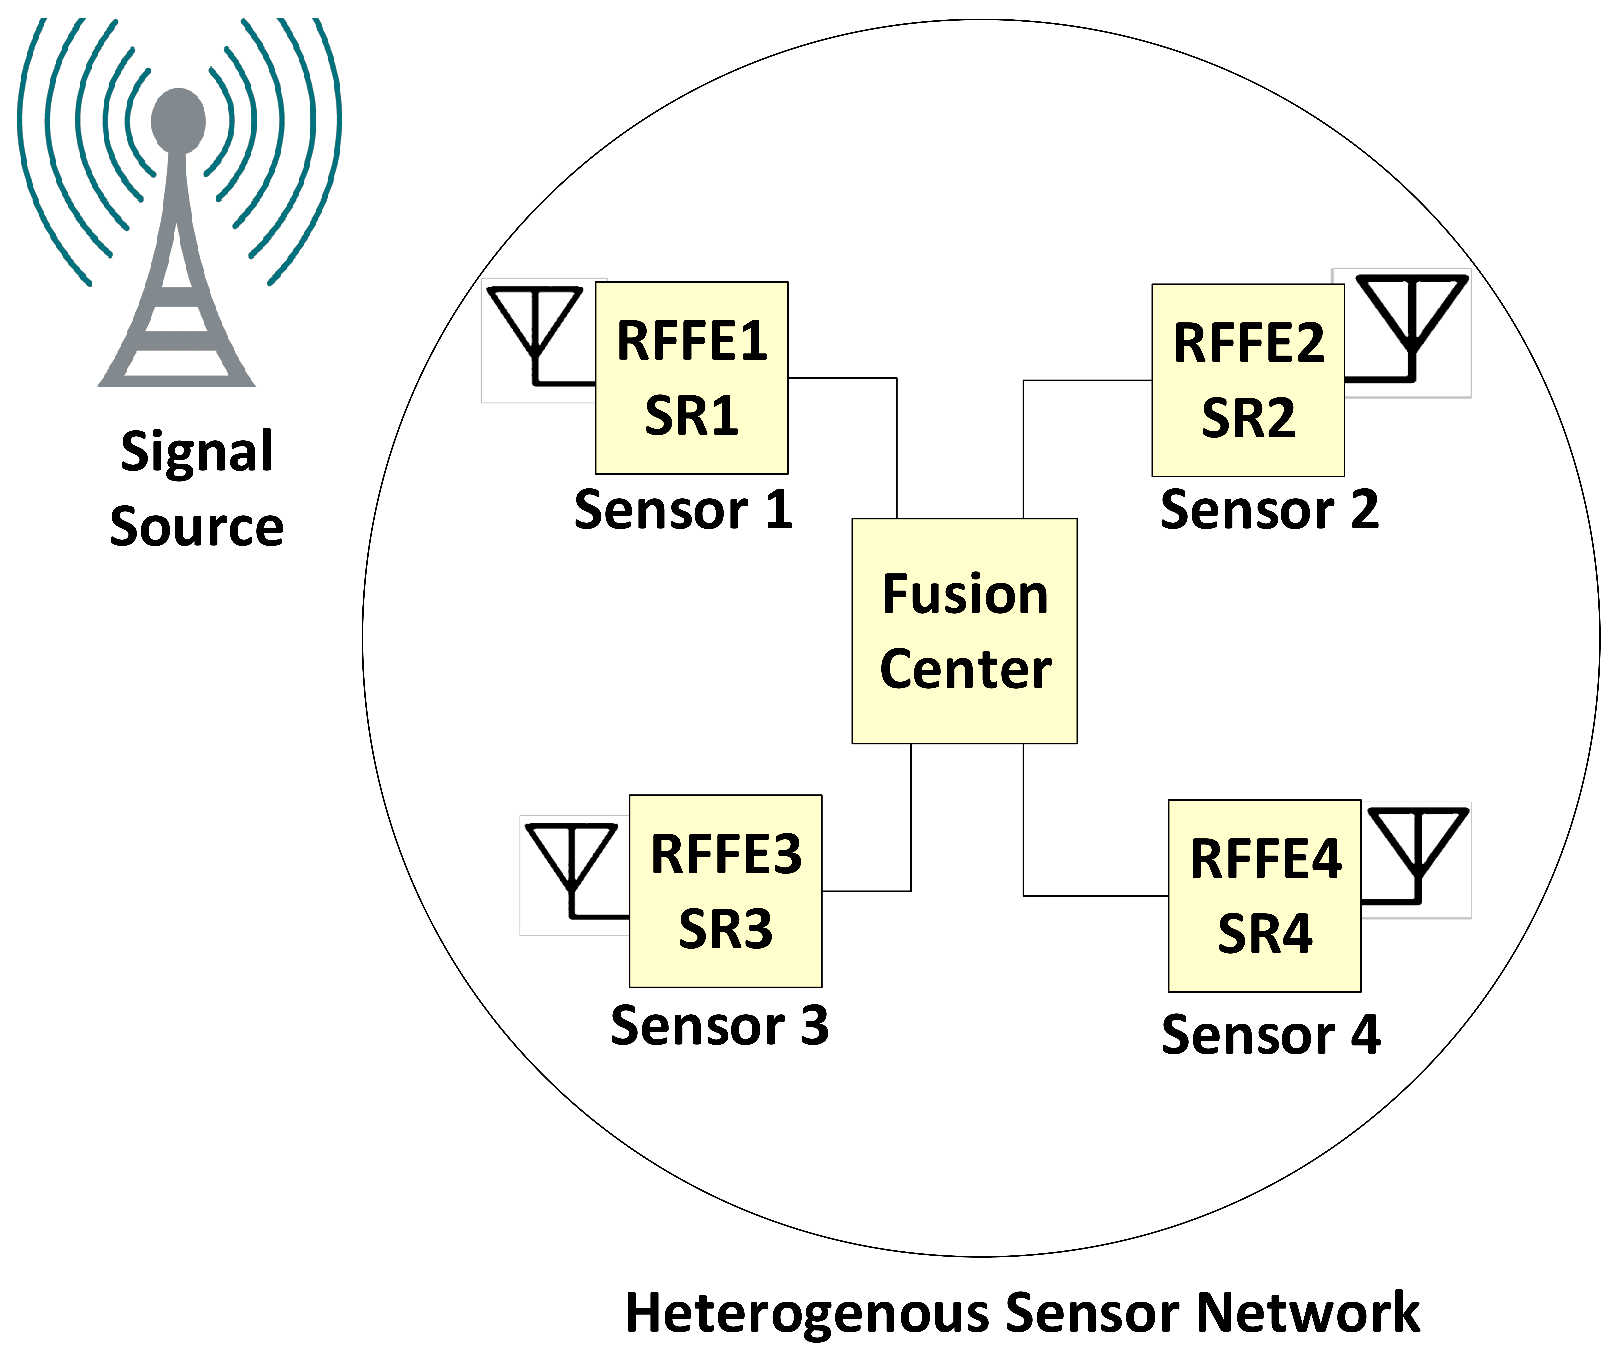
\includegraphics[width=\textwidth,keepaspectratio]{images/Gill/figs/introdiag.eps} 
\caption{Heterogeneous sensor network employing cooperative spectrum sensing. $RFFE_i$ and $SR_i$ represents different front end and sampling rates for the SDR units.}
\label{fig:css}
\end{figure}

\section{State of the Art}

In the open literature, most channel modeling techniques have considered open areas for high speed trains~\cite{inplter5,inplter6}, while relatively little research has been conducted for trains operating in tunnel environments. Due to various challenges presented by tunnel environments, it is important to derive a channel model for LTE-R involving high speed trains. In this thesis, we analyze the effects of high Doppler shift and multipath propagation due to tunnel environments. Experimental studies conducted inside tunnel environments have shown that the field amplitude distribution fits smoothly over a Rician distribution~\cite{inplter8}. Several research efforts have been conducted for large-scale and small-scale fading characteristics for wideband communication systems inside tunnel environments. To the best of the author’s knowledge, none of these studies have been conducted for LTE-R, which employs Orthogonal Frequency Division Multiplexing (OFDM) signals for data transmission inside tunnels. The large Doppler shifts caused by high speed trains will potentially lead to ambiguity when extracting the carrier frequency, which can potentially increase the BER~\cite{inplter9}. Therefore, it is important to study the effects of high Doppler shift and multipath fading for LTE-R communications in tunnel environments such that equalizers can be design efficiently.

% Heterogeneous Networks state-of-the-art..
The cooperative spectrum sensing testbed using normalized energy detection has been implemented and and compared with both soft and hard data fusion schemes. Both soft data fusion and hard data fusion have been extensively studied in the literature~\cite{arhtn9,inphtn10,arhtn11}, with several algorithms being implemented for each scheme. In a hard decision approach, each local decision statistic from a sensor node is transmitted to an fusion center (FC) via overhead channels. The FC merges the sensing data and makes a global decision based on various algorithms such as majority rule, OR rule, and AND rule~\cite{inhtn12}. For a soft decision scheme, each sensor unit (SU) sends its local sensing data to the FC, which makes decision based on a global test statistic $G$. Soft decision combining improves the cooperative gain but it also possesses several limitations. With an infinite bandwidth, the real floating values can be transmitted to the FC, which can lead to a reliable decision mechanism. However, due to bandwidth constraints we have to quantize the data and this leads to error in the energy values. In hard decision combining, we can just transmit the decisions of the sensor nodes to the FC, which can be binary values where ''1'' indicating that signal source is present and ''0'' indicating that a signal source is absent.
\section{Thesis Contributions}
This thesis possesses the following contribution to the cognitive radio communications and railway communications field:

\begin{itemize}
\item A performance assessment and simulation of LTE-R communications in a tunnel environment experiencing severe fading.

\item Dynamic K-factor for a tunnel environment is derived using the classical two-ray propagation model~\cite{booklter11} and is used to build Rician fading model for the tunnel.

\item A cooperative spectrum sensing hardware prototype with normalized energy detection using both soft data fusion and hard data fusion implemented on available software defined radios.

\item For soft data fusion, Maximum Normalized Energy (MNE) and Equal Gain Combination (EGC) algorithms are used. Hard data fusion is also implemented using majority rule, AND, and OR approaches. Both USRP N210s~\cite{usrp} and RTL-SDRs~\cite{rtlsdr} are employed for the implementation of the heterogeneous sensor network.
\end{itemize}


\section{Thesis Organization}
This thesis is organized into the following chapters: Chapter~\ref{chapter2} discusses the smart railway communication system in detail and provides necessary understanding of LTE-R communication system, positive train control (PTC), wireless broadband (WiBro), spectrum regulation. Chapter~\ref{chapter3} provides background knowledge on heterogeneous cooperative spectrum sensing and focuses on heterogeneous networks, cooperative spectrum sensing, and software-defined radios. Chapter~\ref{chapter4} discusses the proposed LTE-R implementation and its results in a tunnel environment. Channel impairments and two-ray propagation model are also discussed in details.  In Chapter~\ref{chapter5}, the proposed implementation of a heterogeneous cooperative spectrum sensing (CSS) test-bed and results are discussed. Chapter~\ref{conclusion} concludes this thesis, summarizing the accomplishments and outlines possible future work.

\section{List of Related Publications}
The following publications resulted from the activities of this thesis research:
\begin{itemize}
\item K. S. Gill and A. M. Wyglinski, "Heterogeneous Cooperative Spectrum Sensing
Test-Bed Using Software-Defined Radios," in Vehicular Technology Conference (VTC Fall), 2017 IEEE 86th, Sept 2017.

\item K. S. Gill, P.V.R Ferreira and A. M. Wyglinski, "Performance Analysis of High Speed Railways Communications Inside a Tunnel Using LTE-R," in Vehicular Technology Conference (VTC Fall), 2017 IEEE 86th, Sept 2017.

\end{itemize}



\chapter{Introduction}
\label{ch:introduction}
\section{Motivation}
Gradually we are moving towards context awareness among automotive devices where the vehicles are aware of their neighborhood. In modern railway applications, a huge amount of wireless communications is used for safety features such as train collision avoidance and railway management. To enhance reliability and safety of Railway systems, while increasing accessibility and productivity, modern railway operations rely on an ever increasing amount of exchange of information between different trains, i.e., train-to-train (T2T) and train-to-ground (T2G). The integration of all of these heterogeneous wireless networks deployed in the railway domain constitutes a key technical challenge. These challenges can potentially be answered by Cognitive Radio (CR) technologies, which can offer interoperability, reliability, dynamic spectrum access, and both lower deployment and maintenance costs. Two research projects currently underway for cognitive radio enabled railway communication include the following:

\begin{itemize}

\item Cognitive Radio for Railway Through Dynamic and Opportunistic Spectrum Reuse (CORRIDOR)~\cite{corridor} is a French research project that targets opportunistic spectrum access for railways. Due to the rapid increase in demand for future railways in terms of control operations as well as providing high speed internet connectivity to the passengers, more bandwidth and spectrum is needed for railway communications.

\item Rail-CR project~\cite{5621621} is a US-based railway system project where the main effort is focused on implementing a positive train control (PTC) technology designed to equip trains with wireless communication capabilities. The project aims to allow trains to communicate with wayside wireless stations while moving to supply important information such as speed and direction in order to improve safety and operations of the railway system.

\end{itemize}

In this thesis, we have designed and implemented two prototypes to further the advancement of smart railway communication systems. In the first test-bed, we have analyzed the performance of high speed train (HST) systems in a tunnel environment. In recent years, the use of trains have witnessed tremendous growth due to their high speeds, which has led to the demand for reliable wireless communication systems with these transportation systems. The development of a reliable wireless network for high speed trains is not a simple task and it is still an emerging technology. Global System for Mobile Communication for Railways (GSM-R)~\cite{trlter1}, was a wireless communications standard designed for high speed trains, but it turned out not to be reliable enough and possess several limitations. Subsequently, LTE-R~\cite{trlter2} proposed a promising solution for achieving broadband data rates in high speed trains that can overcome various GSM-R limitations~\cite{arlter3,inplter4}. 

LTE-R is a high speed communication standard based on the existing LTE system architecture~\cite{inplter4}. There has been several studies regarding the assessment of LTE-R as a viable choice for next generation high speed communications for railway applications~\cite{inplter5,inplter6}. Most LTE systems operate at 1.8 GHz -- 2.6 GHz bands, which possesses a high propagation loss and severe fading effects. Highly mobile trains inside tunnel environments makes the design of reliable communication links very challenging. To achieve reliable radio coverage inside tunnels, leaky feeder cables have been proposed~\cite{arlter7}. With LCX, more uniform coverage can be achieved and installation is also comparatively simple. Each slot in the cable is equivalent to an antenna, which can transmit and receive signals. Figure~\ref{fig:ltertunnel} shows the LOS propagation environment inside a tunnel for a high speed train with velocity $v$.
  
\begin{figure}[!ht]
\centering
\includegraphics[width=0.8\textwidth,keepaspectratio]{images/Gill/lte_figs/3dtunnel.eps} 
\caption{High speed train inside a tunnel for LTE-R. $D_{LOS}$ is the distance between transmitter and receiver, $d$ is the distance between the LCX cable transmission slots.}
\label{fig:ltertunnel}
\end{figure}

The second proposed contribution of this thesis is the design and implementation of a GNU Radio based software-defined radio network performing cooperative spectrum sensing. Smart railway communication system requires large bandwidth in order to support the high data-rate applications. This has facilitated the research in dynamic spectrum access (DSA)~\cite{arhtn2,arhtn3} for efficient utilization of spectrum resources to sustain billions of Internet of Things (IoT) devices. There has been a significant increase in the study of cognitive radios for efficiently utilizing the electromagnetic spectrum. It has been observed that the spectrum occupancy is not uniform across all frequency bands, resulting in numerous spectral white spaces~\cite{bookhtn1}. To opportunistically access these idle channels, spectrum sensing is considered to be a significant technology for enabling DSA. Although several spectrum sensing techniques have been proposed in the open literature, energy detection is widely used due to its low implementation complexity~\cite{arhtn4}. We discuss some of the spectrum sensing techniques along with energy detection below:
\begin{itemize}
\item In \textit{energy detection} (ED), the energy of the signal is detected in the frequency location and based on the threshold value we decide whether the signal is present or absent.

\item \textit{Cyclostationary Feature Detection} is a complex scheme to implement compared to ED and it is mostly used when we need to also classify the signal present based on their modulation scheme.

\item When secondary user has \textit{apriori} knowledge of primary user signal, \textit{matched  filter} (MF)  detection  is  applied. Detection by using matched filter needs less detection time compared to ED but primary user information is required.
\end{itemize}

These spectrum sensing techniques can be used in a non-cooperative manner but it is very challenging to get an accurate estimate using a single-sensor system within a practical fading environment. Various non-idealities, such as shadowing, multipath, and fluctuating noise variance, can make it difficult to detect the primary user~\cite{inphtn5,inphtn6}. Cooperative spectrum sensing can mitigate the effects of multipath and shadowing by utilizing the spatial and temporal diversity of a multiple radio network~\cite{inphtn7,inphtn8}. In cooperative spectrum sensing, each sensor node collects the spectral data and transmits it to a fusion center (FC) for decision making. Figure~\ref{fig:css} shows how a heterogeneous sensor network exploits the spatial diversity. 

\begin{figure}[!ht]
\centering
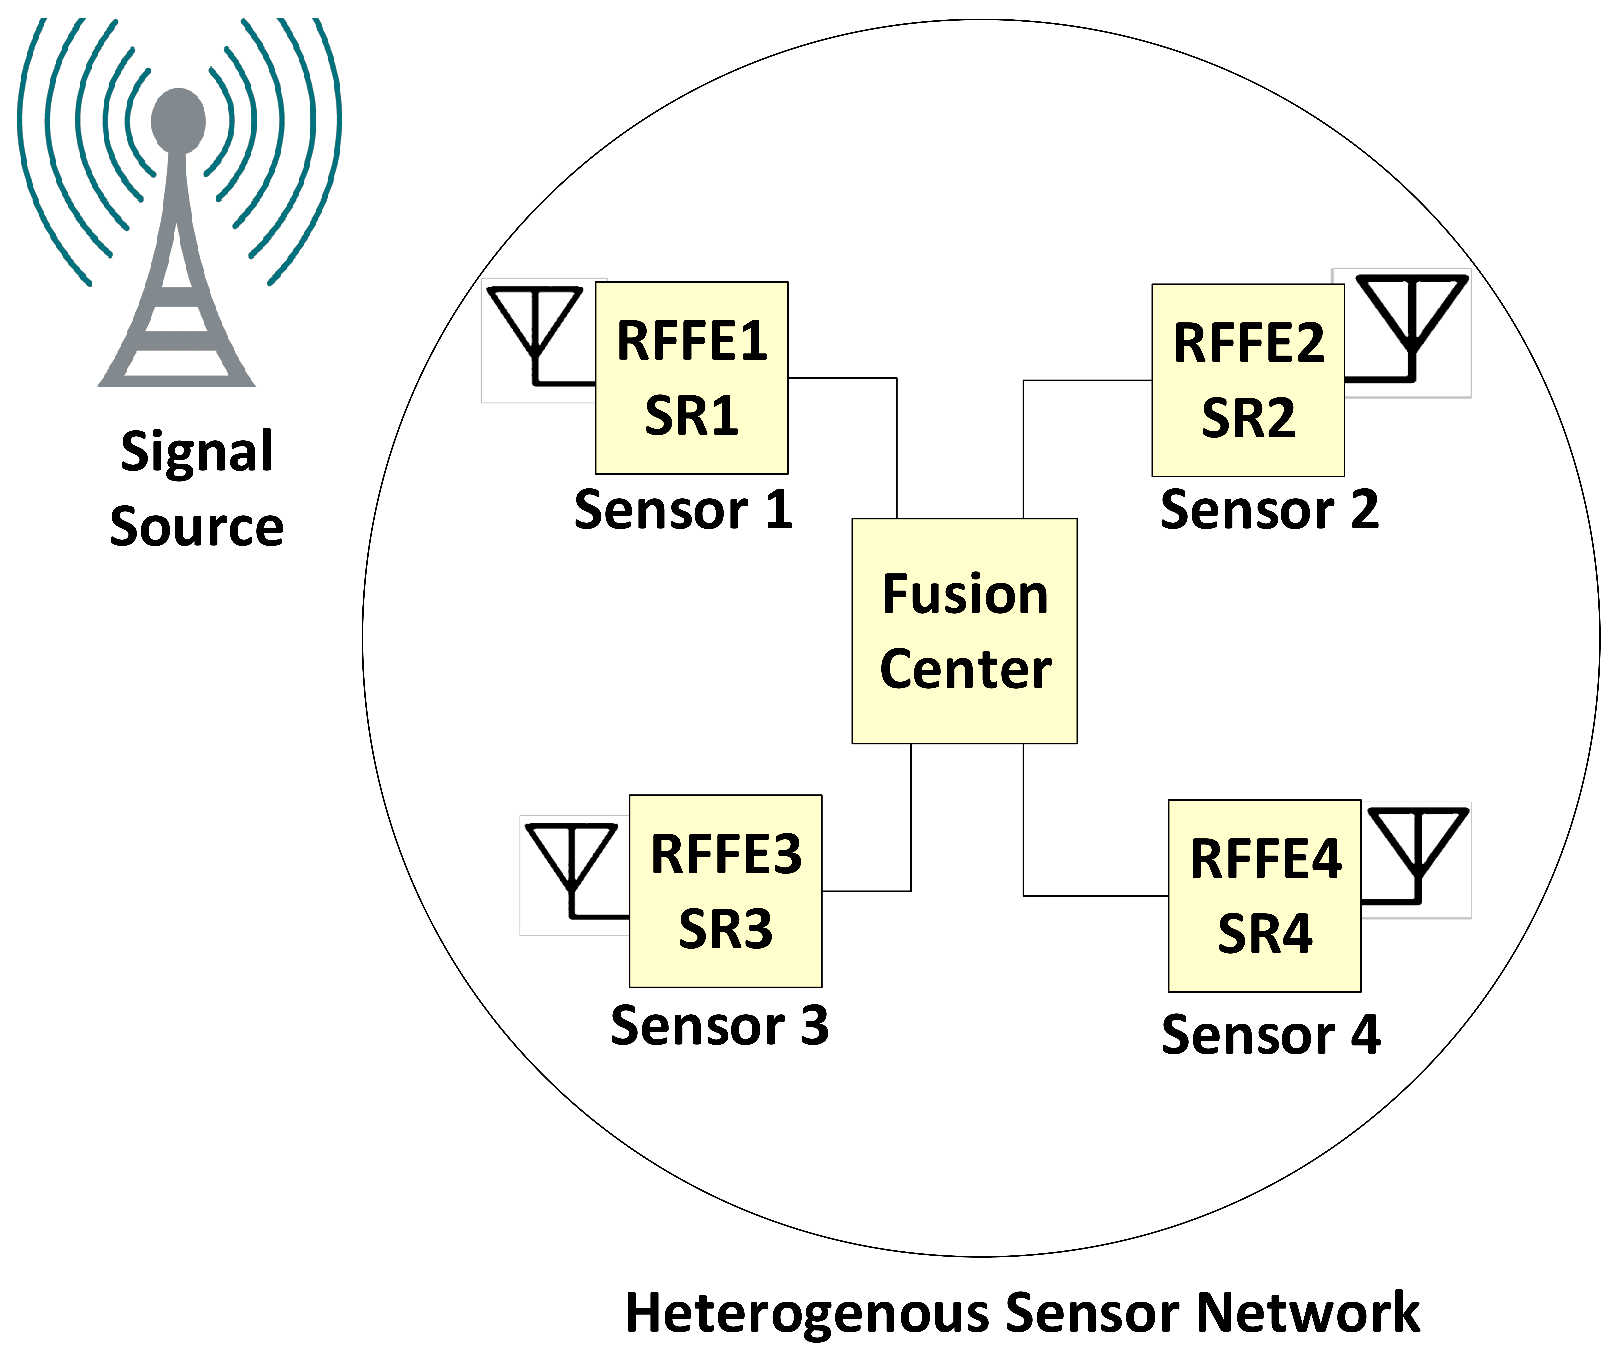
\includegraphics[width=\textwidth,keepaspectratio]{images/Gill/figs/introdiag.eps} 
\caption{Heterogeneous sensor network employing cooperative spectrum sensing. $RFFE_i$ and $SR_i$ represents different front end and sampling rates for the SDR units.}
\label{fig:css}
\end{figure}

\section{State of the Art}

In the open literature, most channel modeling techniques have considered open areas for high speed trains~\cite{inplter5,inplter6}, while relatively little research has been conducted for trains operating in tunnel environments. Due to various challenges presented by tunnel environments, it is important to derive a channel model for LTE-R involving high speed trains. In this thesis, we analyze the effects of high Doppler shift and multipath propagation due to tunnel environments. Experimental studies conducted inside tunnel environments have shown that the field amplitude distribution fits smoothly over a Rician distribution~\cite{inplter8}. Several research efforts have been conducted for large-scale and small-scale fading characteristics for wideband communication systems inside tunnel environments. To the best of the author’s knowledge, none of these studies have been conducted for LTE-R, which employs Orthogonal Frequency Division Multiplexing (OFDM) signals for data transmission inside tunnels. The large Doppler shifts caused by high speed trains will potentially lead to ambiguity when extracting the carrier frequency, which can potentially increase the BER~\cite{inplter9}. Therefore, it is important to study the effects of high Doppler shift and multipath fading for LTE-R communications in tunnel environments such that equalizers can be design efficiently.

% Heterogeneous Networks state-of-the-art..
The cooperative spectrum sensing testbed using normalized energy detection has been implemented and and compared with both soft and hard data fusion schemes. Both soft data fusion and hard data fusion have been extensively studied in the literature~\cite{arhtn9,inphtn10,arhtn11}, with several algorithms being implemented for each scheme. In a hard decision approach, each local decision statistic from a sensor node is transmitted to an fusion center (FC) via overhead channels. The FC merges the sensing data and makes a global decision based on various algorithms such as majority rule, OR rule, and AND rule~\cite{inhtn12}. For a soft decision scheme, each sensor unit (SU) sends its local sensing data to the FC, which makes decision based on a global test statistic $G$. Soft decision combining improves the cooperative gain but it also possesses several limitations. With an infinite bandwidth, the real floating values can be transmitted to the FC, which can lead to a reliable decision mechanism. However, due to bandwidth constraints we have to quantize the data and this leads to error in the energy values. In hard decision combining, we can just transmit the decisions of the sensor nodes to the FC, which can be binary values where ''1'' indicating that signal source is present and ''0'' indicating that a signal source is absent.
\section{Thesis Contributions}
This thesis possesses the following contribution to the cognitive radio communications and railway communications field:

\begin{itemize}
\item A performance assessment and simulation of LTE-R communications in a tunnel environment experiencing severe fading.

\item Dynamic K-factor for a tunnel environment is derived using the classical two-ray propagation model~\cite{booklter11} and is used to build Rician fading model for the tunnel.

\item A cooperative spectrum sensing hardware prototype with normalized energy detection using both soft data fusion and hard data fusion implemented on available software defined radios.

\item For soft data fusion, Maximum Normalized Energy (MNE) and Equal Gain Combination (EGC) algorithms are used. Hard data fusion is also implemented using majority rule, AND, and OR approaches. Both USRP N210s~\cite{usrp} and RTL-SDRs~\cite{rtlsdr} are employed for the implementation of the heterogeneous sensor network.
\end{itemize}


\section{Thesis Organization}
This thesis is organized into the following chapters: Chapter~\ref{chapter2} discusses the smart railway communication system in detail and provides necessary understanding of LTE-R communication system, positive train control (PTC), wireless broadband (WiBro), spectrum regulation. Chapter~\ref{chapter3} provides background knowledge on heterogeneous cooperative spectrum sensing and focuses on heterogeneous networks, cooperative spectrum sensing, and software-defined radios. Chapter~\ref{chapter4} discusses the proposed LTE-R implementation and its results in a tunnel environment. Channel impairments and two-ray propagation model are also discussed in details.  In Chapter~\ref{chapter5}, the proposed implementation of a heterogeneous cooperative spectrum sensing (CSS) test-bed and results are discussed. Chapter~\ref{conclusion} concludes this thesis, summarizing the accomplishments and outlines possible future work.

\section{List of Related Publications}
The following publications resulted from the activities of this thesis research:
\begin{itemize}
\item K. S. Gill and A. M. Wyglinski, "Heterogeneous Cooperative Spectrum Sensing
Test-Bed Using Software-Defined Radios," in Vehicular Technology Conference (VTC Fall), 2017 IEEE 86th, Sept 2017.

\item K. S. Gill, P.V.R Ferreira and A. M. Wyglinski, "Performance Analysis of High Speed Railways Communications Inside a Tunnel Using LTE-R," in Vehicular Technology Conference (VTC Fall), 2017 IEEE 86th, Sept 2017.

\end{itemize}




%% Heterogeneous CSS intro
\chapter{Smart Railway Communication System}
\label{chapter2}

There has recently been growing interest in high speed railway (HSR) communication systems. This growing demand in HSR communication has led to significant activity with respect to next generation wireless communication systems applied to railway environments. Current GSM-railway (GSM-R) technology is not sufficient for satisfying the demand for large data rate applications and quality-of-service (QoS) requirements, which has subsequently led to development of Long Term Evolution for railways (LTE-R)~\cite{7553613}. LTE-R is based on the LTE architecture~\cite{7553613} and has been championed as the future of the smart railway communication systems. LTE-R provides a more efficient network architecture compared to GSM and has a reduced packet delay. It is also based on a well-established and off-the shelf communication system that provides standardized interworking mechanisms and compatibility with GSM-R. In the following sections, we discuss positive train control (PTC), wireless broadband (WiBro), train-to-train (T2T), and train-to-ground (T2G) communication, Long Term Evolution for Railways (LTE-R) communication system, spectrum regulation for railway communication systems, LTE-R services for railways, and leaky coaxial cable (LCX), all of which are important technologies for achieving smart railway transportation system.

\section{Positive Train Control}
Positive Train Control (PTC) is designed for the monitoring and controling of train movements in order to provide advanced safety operations with the help of modern wireless communication technology. The key idea behind PTC is the constant flow of information to the train about its location as well as warning engineers about train speeds in order to prevent derailment~\cite{nytimes}. Managing track occupancies through centralized route and interlocking logic, enforcing permanent and temporary speed limits for the train, and real-time localization of the train are some of the basic features implemented in PTC. 

\begin{figure}[!ht]
\centering
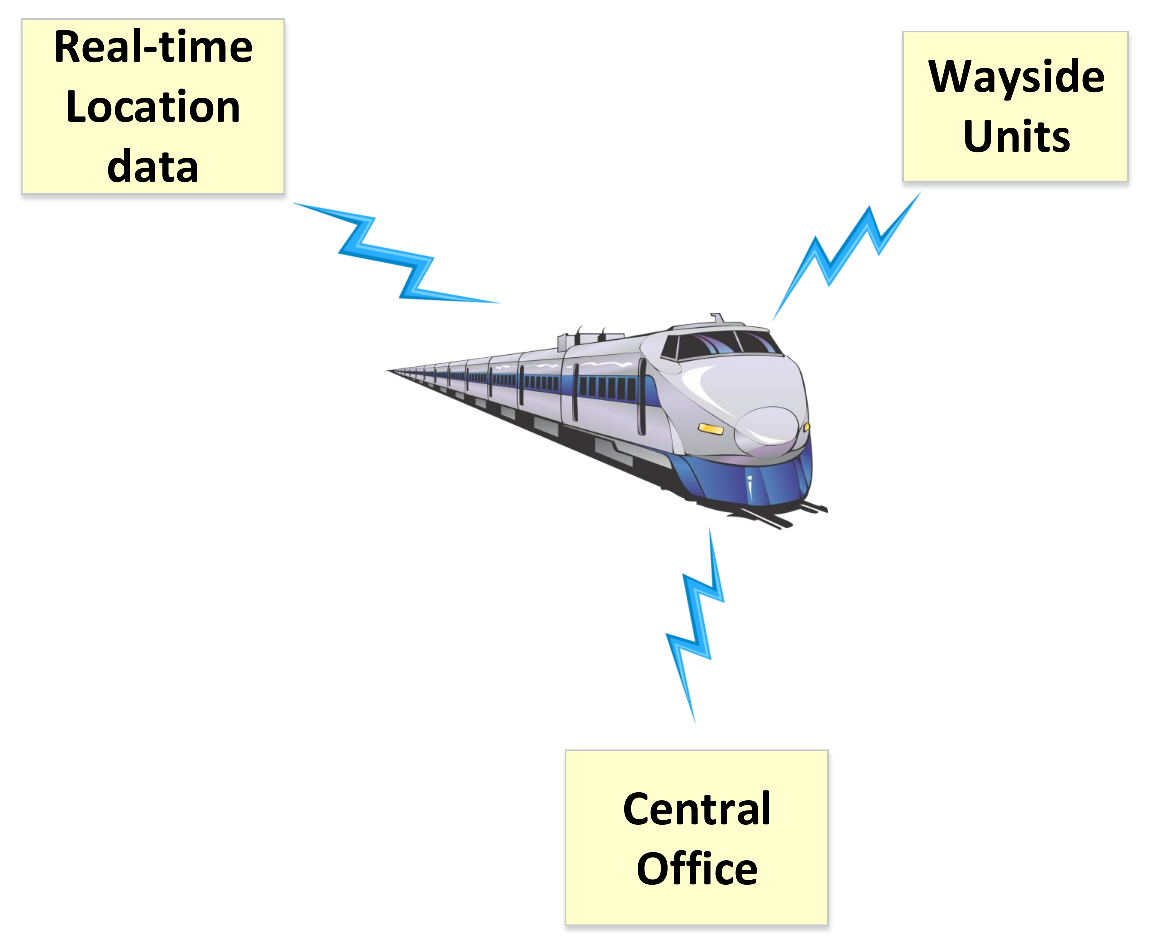
\includegraphics[width=\textwidth,height=10cm,keepaspectratio]{images/Gill/5G/ptc.eps} 
\caption{Architecture of Positive Train Control consisting of wayside units, central office and real-time GPS information. All these technologies assist PTC in achieving advance control and safety of the trains.}
\label{ptc}
\end{figure}


Figure~\ref{ptc} provides a generalized viewpoint of the PTC architecture; where the train receives the flow of information through various systems using wireless communication links. The primary means of determining location for the train is by using differential GPS, which can continuously compare its position with the stored position of speed restriction and work zones~\cite{5338992}. The Central Office (CO) regularly monitors trains, exchanging information with train management computers (TMC), and gathering precise speed and position information. The CO also collects information regarding train orders, number of cars, weight, route and track characteristics along the route, including speed restrictions, curves, grades and crossing. All wayside equipment are continuously monitored by PTC, where they issue alerts in cases when an automatic crossing gate is not working or a hot box detector senses several axles slightly above a certain temperature level. It also applies corrective action in cases where there are reports of a possible track breakage due to extreme heat or a flood.

\section{Wireless Broadband (WiBro)}

Wireless Broadband (WiBro) is a mobile broadband wireless access (BWA) service which had its first public demonstration in December 2005 and has been in service in South Korea since June 2006. WiBro was developed as a mobile BWA solution in Korea and was based on the IEEE 802.11e WiMax standard~\cite{wibro}. It is a subset of the consolidated version of the IEEE Standard 802.16-2004 (fixed wireless specifications), P802.16e (enhancements to support mobility), and P802.16-2004/Cor1 (corrections to IEEE Standard 802.16-2004). The profiles and test specifications of WiBro have been harmonized with the WiMAX Forum's mobile WiMAX profiles and test specification, resulting in a convergence of the two standards.


\begin{figure}[!ht]
\centering
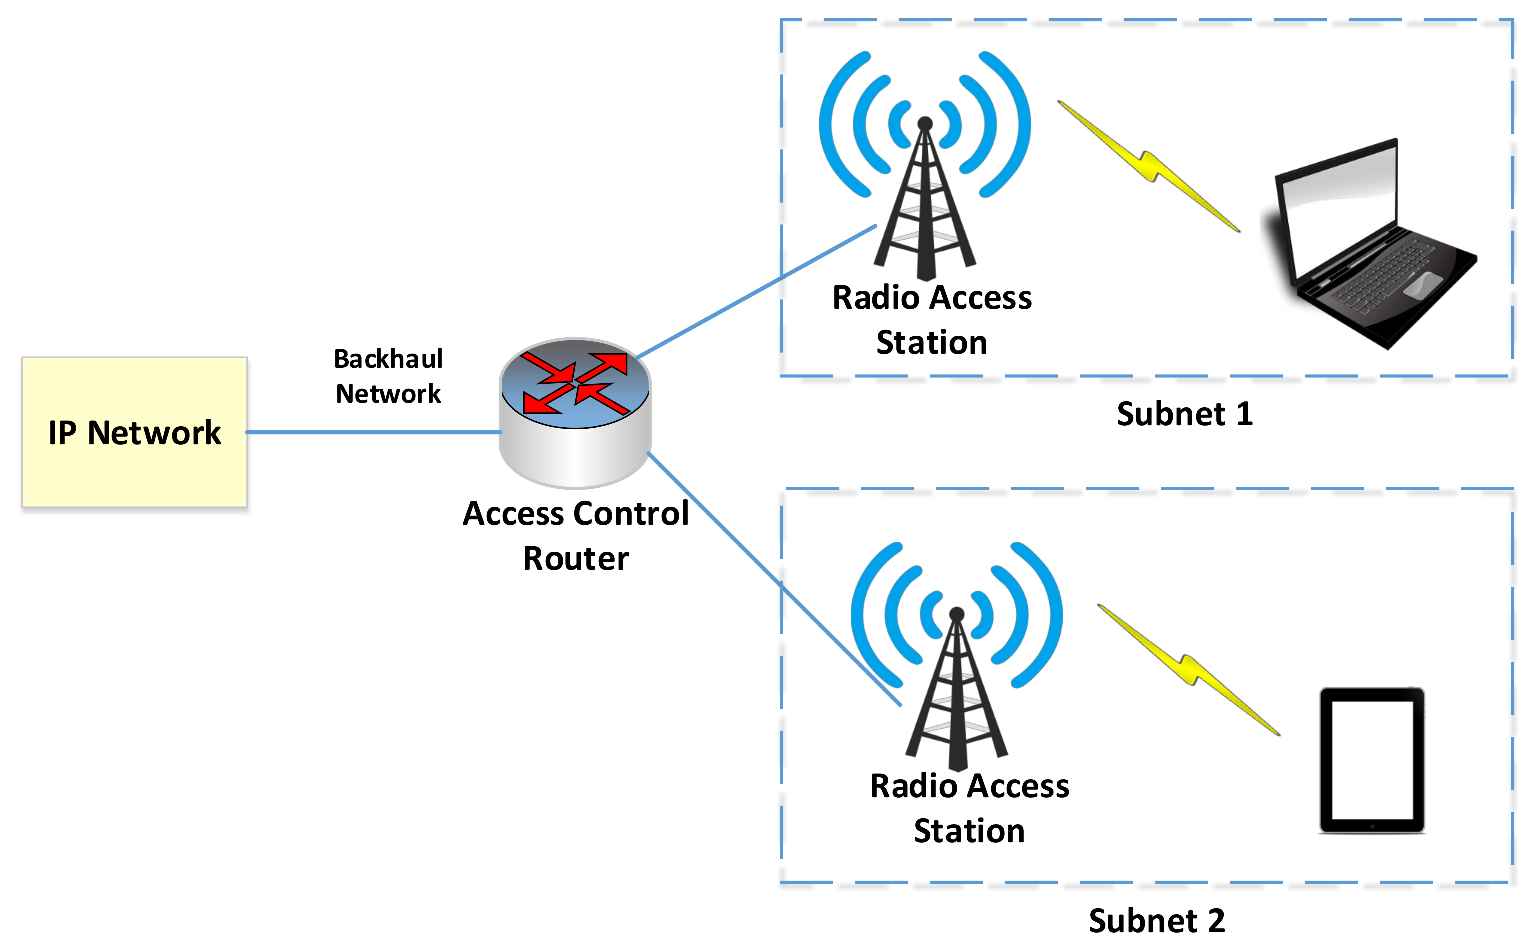
\includegraphics[width=\textwidth,height=10cm,keepaspectratio]{images/Gill/5G/wibro.eps} 
\caption{Korean Wireless Broadband (WiBro) system architecture for high speed internet connectivity. WiBro is an all IP-based network, which uses ACRs to connect the backbone network with radio access station.}
\label{wibro}
\end{figure}

Figure~\ref{wibro} describes the architecture of BWA-based WiBro communication system in the Phase I standardization~\cite{wibro}. The WiBro network consists of Access Control Routers (ACR), which connects the backbone network with a Radio Access Station (RAS). The RAS is the interface between the mobile nodes and the core network at the physical layer, and it controls the radio resources at the data link layer in conjunction with an ACR. The key distinction of WiBro from conventional cellular networks is that the Internet Protocol (IP) is used between an ACR and RASs, as well as between ACRs. WiBro uses Time Division Duplexing (TDD) or Frequency Division Duplexing (FDD) for duplexing and Orthogonal Frequency Division Multiple Access (OFDMA) for robustness against fast fading and narrow-band co-channel interference.


\section{LTE-R Communication System}

The development of a reliable wireless network for high speed trains is not a simple task and it is still an emerging technology. Global System for Mobile Communication for Railways (GSM-R)~\cite{trlter1} was a wireless communications standard designed for high speed trains, but it turned out not to be reliable enough and possessed several limitations. The data rates for voice services, which can reach up to 9.6 kbps, was unable to meet the increasing demands of high-rate data transmission for railways communication. Furthermore, the limited data rate and quality of service (QoS) requirements were not sufficient to support cellular communications. Subsequently, LTE~\cite{trlter2} proposed a promising solution for achieving broadband data rates, flexible bandwidth allocation, and high spectral efficiency in high speed trains that can overcome various GSM-R limitations~\cite{arlter3,inplter4}.

\begin{figure}[!ht]
\centering
\includegraphics[width=\textwidth,keepaspectratio]{images/Gill/lte_figs/lter_architecture.eps} 
\caption{Proposed LTE-R Architecture for next generation High-speed Railways consisting of EPA and E-UTRAN.}
\label{ltearch}
\end{figure}

LTE-R is a high speed communication standard based on the existing LTE system architecture~\cite{inplter4}. There has been several studies regarding the assessment of LTE-R as a viable choice for next generation high speed communications for railway applications~\cite{inplter5,inplter6}. Conventional LTE includes an Evolved Packet Core (EPC) network and a radio access network referred to as an Evolved Universal  Terrestrial  Radio  Access  Network (E-UTRAN). The  Internet  Protocol (IP)-based  EPC  supports  seamless handovers for both voice and data to cell towers, and each E-UTRAN cell will support high data and voice capacity by high-speed  packet  access  (HSPA).  As  a  candidate for the next-generation  communication  system  of  HSR,  LTE-R  inherits all the important features of LTE and provides an extra radio access system to exchange wireless signals with onboard  units (OBUs)  and to match HST-specific  needs. Figure~\ref{ltearch} shows the proposed architecture of LTE-R according to~\cite{trlter2}, which shows the core network of LTE-R is backward compatible with GSM-R. The network architecture of LTE-R is similar to that of LTE/SAE, with  Evolved Universal Terrestrial Radio Access Network (E-UTRAN) being the access network structure of LTE-R. The Evolved-Node B (eNodeB) units communicate directly with UEs in a similar fashion to a base transceiver station (BTS) in GSM networks. It performs the transmission and reception of data packets using Orthogonal Frequency Division Multiplexing Access (OFDMA) for downlink and Single Carrier Frequency Division Multiple Access (SC-FDMA) for uplink across the PHY layer. At the same time, as without the base-station controller (BSC), it also has radio  resource  control and wireless  mobility  management functions.  The eNodeB units can be connected to the network router directly without additional intermediate control nodes, such as the BSC in GSM-R~\cite{tingting2010high}. The main difference between EPC and the core network of GSM-R is that the EPC is an all-IP mobile core network.

\begin{table}[h!]
\caption{Comparison of system parameters between GSM-R , LTE and LTE-R.}
\begin{adjustbox}{width=\textwidth, center=\textwidth}
\begin{tabular}{| c | c | c | c |}
\toprule
System Parameters & GSM-R & LTE & LTE-R\\ 
\midrule
Frequency & \shortstack{Uplink: 876--880 MHz\\downlink: 921--925 MHz} & 800, 1800, 2600 MHz & 450, 800, 1400, 1800 MHz \\  
Capacity  & 0.2 MHz & 1.4-20 MHz & 1.4-20 MHz\\ 
Modulation  & GMSK & QPSK/16-QAM/64-QAM & QPSK/16-QAM\\ 
MIMO  & No  & 2x2, 4x4  & 2x2\\ 
Cell Range  & 8 Km  & 1-5 Km & 4-12 Km \\ 
Data Rates (DL/UL)  & 172/172 Kbps  & 100/50 Mbps & 50/10 Mbps\\ 
\bottomrule
\end{tabular}
\end{adjustbox}
\label{ltertable}
\end{table}

Conventional LTE networks are different compared to LTE-R in several ways, such as architecture, system parameters, network layout, services, and quality of service (QoS). Table~\ref{ltertable} summarizes the LTE-R parameters and describes the differences between LTE, GSM-R, and LTE-R. Since the LTE-R environment possesses very severe fading and high Doppler shift, it is configured for QoS rather than higher data rates. Therefore, QPSK modulation is used for most sub-carriers, and the number of packet re-transmissions must be kept low, which is achieved with the User Datagram Protocol (UDP).


\section{Spectrum Regulation for LTE-R}

Departing from the technical issues for a moment, we will now discuss the important interactions that smart railways will encounter with respect to spectrum policy and allocation defined by the Federal Communications Commission (FCC). The spectrum allocated for cellular technologies is already saturated in peak markets due to massive amounts of wireless services and networks. Figure~\ref{specalloc} illustrates the issue of potential spectrum scarcity in the wireless cellular bands using the frequency allocation chart of the United States~\cite{fcc}. Frequencies located at the lower portion of the spectrum can be used for wide coverage, mobility support, and control signaling while the higher portion of frequencies can be used for high data rate applications. This requires a new approach to spectrum policy and allocation methods for smart railway standardization.

\begin{figure}[!ht]
	\centering
\includegraphics[width=\textwidth,keepaspectratio]{images/Gill/5G/specalloc.eps}
	\caption{Federal Communications Commission (FCC) spectrum allocation chart~\cite{fcc}.}
	\label{specalloc}
\end{figure}

Cognitive radio is a promising technology that can solve the spectrum shortage problem resulting from the rapid increase in wireless networks and mobile devices. Recent advancements in software-defined radio technology and edge computing have enabled new Cognitive Radio Network (CRN)  capabilities and, along with some adjustments in its operation, will be a key technology for LTE-R heterogeneous network deployment. Cognitive Radio using software defined radio technology is considered to be one of the key technologies for improving the utilization of congested radio spectrum~\cite{rusek2013scaling}. Integrating CR technology into an LTE-R system is motivated by the fact that a large portion of the radio spectrum is underutilized most of the time~\cite{7553613}. For achieving data rates on order of gigabits per second, we need to make efficient use of the available spectrum, which can be achieved by using CRNs. CRNs are a secondary wireless access system that can share frequency bands with the incumbent primary wireless access system, either on an interference-free basis or an interference-tolerant basis. The CRN should be aware of
the surrounding radio environment and be capable of regulating its transmission accordingly. For interference-free CRNs, CR users are allowed to borrow spectral resources only when licensed users do not use them. The key for enabling interference-free CRNs is figuring out how to detect the spectrum holes (white spaces) that are located across the spectrum and enable dynamic spectrum access (DSA)~\cite{wyglinski2009cognitive}.

CR receivers should first monitor and allocate the unused spectrum via spectrum sensing (energy detection (ED), covariance absolute value (CAV) detection, etc.)~\cite{wyglinski2009cognitive} or by combining spectrum usage from geolocation databases and feed this information back to the central CR controller. A coordinating mechanism is required for multiple CRNs where they all try to access the same spectrum in order to prevent users colliding with each other while accessing the same spectrum holes. For interference-tolerant CRNs, CR users can share the spectrum resources with a licensed system while keeping the interference below a threshold. In comparison with interference-free CRNs, interference-tolerant CRNs can achieve enhanced spectrum utilization by opportunistically sharing the radio spectrum resources with licensed users, and can also achieve better spectral and energy efficiency. However, it has been shown that the performance of CR systems can be very sensitive to any slight change in user density, interference threshold, and transmission behavior of the licensed system~\cite{haykin2005cognitive}. However, the spectral efficiency can be improved by either relaxing the interference threshold of the primary system or considering only the CR users having short distances to the secondary BS (utilizing the spatial gain). Hybrid CRNs have been proposed in~\cite{hong2010capacity} for adoption in cellular networks in order to explore additional bands and expand the capacity. CRNs can only prove beneficial if the spectrum policies related to LTE-R are implemented in a robust manner. 

\section{Train-to-train (T2T) Railway Communication}

The development of driverless cars has imposed several strict requirements for the safety of passengers and pedestrians. For safety-critical applications, transmission delays need to be less than 10 ms, which is required for intelligent transportation systems (ITS) and vehicular networks~\cite{ge2016vehicular}. While communications for road traffic has been well investigated, with the first standards being defined for smart vehicles (ITS-G5), railway communications have mainly focused on train-to-ground (T2G) communication using GSM-R and LTE-R. Nevertheless, there are still several challenges involved in train-to-train (T2T) communications for frequencies above 1 GHz and high speed operations (up to 500 Km/h), which can potentially lead to severe fading. In~\cite{nterhuber2017wide}, a measurement campaign was performed focusing on wagon-to-wagon measurements (intra-consist) with one high speed train (HST), as well as T2T measurements with two HSTs. A survey of channel measurements and models are presented in~\cite{unterhuber2016survey}. Various simulation and experimental results revealed a trade-off between the proposed performance metrics and system parameters, such as base station (BS) and vehicle densities, radio coverage, and  the  maximum number of hops in a path. With LTE communication technologies being integrated into vehicular networks, the interference will cut down the performance of LTE vehicular networks. When vehicle density is high, the beaconing signals of the vehicular safety applications may easily overload the responsible eNodeB. To handle this issue, these signals should be handled directly between vehicles without  having to go through  the  eNB. In  LTE-Advanced (LTE-A), device-to-device (D2D) communications is considered, where direct message delivery between terminals in proximity to each other is permitted in order to decrease the load of the eNB~\cite{mumtaz2014direct}. 

\begin{figure}[!ht]
	\centering
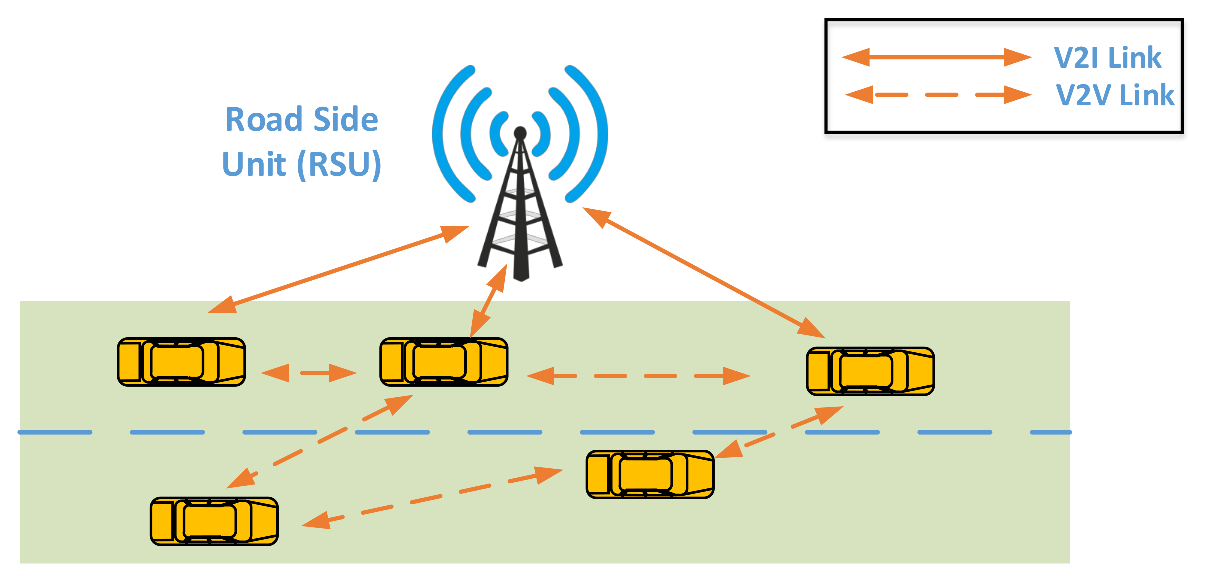
\includegraphics[width=\textwidth,keepaspectratio]{images/Gill/5G/vehiclecomm.eps}
	\caption{Vehicular communication using D2D 5G cellular communication technology.}
	\label{vcomm}
\end{figure}

The infrastructure-aided D2D technologies can serve as a natural approach for enabling reliable and efficient T2T communications without negatively affecting existing cellular systems. To meet the expected performance requirements, such as low transmission delay and high throughput, a new architecture for LTE-R vehicular communication is required. Figure~\ref{vcomm} illustrates how railway communications using the D2D strategy can offload the computation from remote road side units (RRU) to the trains in order to increase spectral efficiency. The communication environment in T2T is different than in D2D due to the high mobility (Doppler shift) of the high speed trains. Network connectivity plays a important role in T2T communication relative to D2D when comparing system throughput. These features can significantly affect D2D resource allocation strategies and system parameters, and thus should be modified for railway communication.

\section{LTE-R Services}
LTE-R provides services to improve security, quality of service (QoS), and efficiency for high speed railways. Several key services include the following:

%\begin{figure}[!ht]
%	\centering
%\includegraphics[width=\textwidth,keepaspectratio]{images/Gill/5G/device2device.eps}
%	\caption{Key LTE-R services required to augment railway security, QoS and efficiency}
%	\label{d2d}
%\end{figure}

\begin{itemize}
\item \textit{Train Control}: Train control (TC) continually monitors trains, exchanges information with Train Management Computers (TMC), and gathers precise speed and position information. TC will have a copy of train orders, number of cars, weight, route and track characteristics along the route, including speed restrictions, curves, grades and crossings. Track authority, \textit{i.e.}, permission to occupy and move on a sector of track, is continuously updated as train control computers issue or modify train orders.

\item \textit{Real-time monitoring}: LTE-R should provide video monitoring of railway track conditions (flaw detection and temperature), as well as railway infrastructure, in order to avoid accidents. The information should be transmitted in real-time with both central controller and HST with minimum delay possible. 

\item \textit{Railway Emergency Communications}: Whenever there is any natural calamity or an emergency situation, an establishment of immediate communications between accident site and rescue center is of the utmost importance. Railway emergency communications systems use railway private networks to ensure rapid deployment and faster responses compared to the existing technologies such as GSM-R. 

\item \textit{Real-time Localization for Trains}: LTE-R should be able to relay the real-time localization information to the central controller such that the efficiency of scheduling trains can be improved. With accurate localization information, train collisions can be avoided and better overall service can be provided to the passengers.

\item \textit{Railway IoT}: With railway Internet-of-Things (IoT), LTE-R can provide services such as real-time query and tracking of trains and goods. It helps to improve the transport efficiency and extend service range. Railway IoT can also help in augmenting the railway safety features.
\end{itemize}

\section{Leaky Coaxial Cable for LTE-R}
Leaky Coaxial Cable (LCX)~\cite{n1974leaky} is an antenna technology designed to deliver radio services in tunnel environment. It consists of small periodic slots to allow radio frequency (RF) signals to escape, which act as extended antenna elements. LCX cables were invented to provide the uniform signal coverage in underground mines where radio coverage can potentially be very limited due to the mine environment~\cite{arlter10}. Recently, leaky coaxial cables have been widely used in the field of railway communication, especially in tunnels~\cite{arlter10}. Leaky feeders are
constructed from coaxial cable, where the outer shield has a series of holes with different shapes and different distances amongst them. The coaxial cable is usually on the order of hundreds of metres long, and it can be installed throughout a building or a tunnel. So far, LCX have been only used to supplement wireless communication systems between a BS and trains, mostly transmitting voice signals. LCX are being used as an alternative solution to distributed antenna systems in indoor environments such as commercial buildings~\cite{motley1983directed,saleh1987distributed} and university buildings, high speed trains, and cars. The LCX radio system is almost noise free and has enough bandwidth to support multiple RF signals carrying voice and data simultaneously. Figure~\ref{fig:leakcoax} shows the conventional leaky coaxial cable along $x$-axis with periodic radiating slots and wave propagation along $z$-axis. Generally, it consists of three parts: Inner conductor, Dielectric material, and inner conductor. LCX has a dual functionality \textit{i.e.}, they can transmit and receive RF signals using their slots. The frequency range for a leaky cable is given by~\cite{cao1999radio}:
\begin{equation}
\dfrac{c}{\sqrt{\varepsilon_r-1)}d}\geq f \leq \dfrac{c}{\sqrt{\varepsilon_r}+1)d}.
\end{equation}
where $c$ is the speed of light in $m/s$, $d$ is the length of the LCX cable, and $\varepsilon_r$ is the relative permittivity of the tunnel walls.
\begin{figure}[!ht]
\centering
\includegraphics[width=\textwidth,keepaspectratio]{images/Gill/lte_figs/leakycoax.eps} 
\caption{Leaky Coaxial Cable used for uniform radio coverage in a Tunnel environment~\cite{arlter10}.}
\label{fig:leakcoax}
\end{figure}

A radio system based on LCX has been deployed in Japan for high speed railways ''Series N700''~\cite{takatsu2007history} to connect the train to the ground network. Wi-Fi access points are chosen for in-train communications with peak data rates of 2 Mbps for uplink and downlink. Although current technologies can provide wireless communication services in HSTs, the capacity of communication system is very low (1--4 Mbps). These data rates are insufficient for next generation wireless communication system where the peak data rates of 0.5 -- 5 Gbps are expected. LTE-R communication system can be implemented for achieving high data rates but it cannot be achieved by using conventional cellular systems. The penetration loss due to the tunnel walls is very high and secondly, the fast moving trains cause large Doppler shifts leading to poor connectivity due to retransmissions. Hence, leaky coaxial cable is potentially the best candidate for achieving extensive internet access inside a tunnel environment for high speed railways.

\section{Summary}
This chapter outlined and examined the topics of positive train control, WiBro, LTE-R communication system and provided a foundation for smart railway communication system. We also discuss the spectrum regulation for LTE-R, T2T railway communication, various services required in LTE-R and finally leaky coaxial cables (LCX) for uniform coverage in a tunnel environment. Next in this thesis, we consider heterogeneous cooperative spectrum sensing (CSS) and how it can be use to augment smart railways. After CSS, we discuss the implementation and results of our proposed test-bed for high speed train and software-defined radios.\\


%% LTE-R analysis intro
\chapter{Heterogeneous Cooperative Spectrum Sensing (CSS)}
\label{chapter3}

This chapter provides the background information needed to understand the chapters that follows. It examines the basic outlines of a heterogeneous networks and how cooperative spectrum sensing (CSS) can help in enhancing the accuracy of signal source estimation. The fusion center (FC) collects the data from the sensor node network and process it to make the reliable decision. Secondly, this chapter investigates various algorithms which can be used in heterogeneous network to estimate signal source. Finally, it also outlines the necessary hardware and software tools used in the implementation of heterogeneous CSS chapter.

\section{Spectrum Sensing}
Spectrum sensing plays a key role in the decision-making part of cognitive radio network. It is required by CR to detect the presence of spectrum white space and also to estimate accurately the presence of incumbent users (PUs). Since the primary users have prerogative on the spectrum band usage, so it is of paramount importance to avoid interfering with the PU. It is very challenging to get an accurate estimate under a practical fading environment based on conventional spectrum sensing techniques. Various non-idealities such as shadowing, multipath and fluctuating noise variance can make it difficult to detect the primary user. In the case of fast  varying  channels over time, some works focus on improving the peformance of spectrum sensing and signal identification~\cite{hassan2012blind,kharbech2013blind,hassan2009automatic}. To combat the Doppler shift caused due to high-speed environments algorithms~\cite{simon2013iterative} have been proposed for channel estimation and equalization. Cooperative spectrum sensing~\cite{ksgill} can be use to tackle lot of the problems caused due to multipath, shadowing and high Doppler shift. In the thesis we tested the performance of cooperative spectrum sensing using soft and hard data fusion schemes on software-defined radio test-bed. The experiment confirmed that cooperation among sensor nodes improved the spectrum sensing performance as a result of increased spatial-temporal diversity in received signal source. The various types of spectrum sensing schemes are discussed below in the following subsections.

\subsection{Energy Detection}
In energy detection (ED) we use the energy spectra of the received signal and compare it against a predefined threshold level to estimate the presence of the signal.In ED scheme we only rely on the energy of the signal in the frequency channel, and no phase information is required. The key advantage of the ED scheme is that it doesn't require any prior information of the signal, i.e. type of modulation scheme, phase information or any other signal parameter. Energy detection can be considered as binary hypothesis testing scheme and is given by~\cite{arhtn4}:

\begin{equation}
	\label{eq:1}
     y(n) = 
     \left\{
     \begin{aligned}
   &w(n),~~~~~~~~~\Hmat_0\\
   &s(n) + w(n),~\Hmat_1
    \end{aligned}
    \right.
\end{equation}
where $y(n)$ represents the received signal, $s(n)$ represents the signal source (PU), and $w(n)$ is the white Gaussian noise $w(n) \sim N(0,\sigma_n^2) $. $\Hmat_0$ describes the hypothesis when there is no signal present, while the hypothesis $\Hmat_1$ is the presence of signal. Figure~\ref{energydet} explains the energy detection scheme in the form of a block diagram. Firstly the analog signal $X(t)$ is converted into digital domain via analog-to-digital (ADC) converter, then the Fast Fourier Transform (FFT) block converts the signal from time domain to frequency domain. We then calculate the magnitude square of the signal and finally we take the average over the N values to compute the decision statistic $\delta $. The $\delta$ is compared with the threshold to estimate the presence or absence of the signal.

\begin{figure}[ht!]
	\centering
	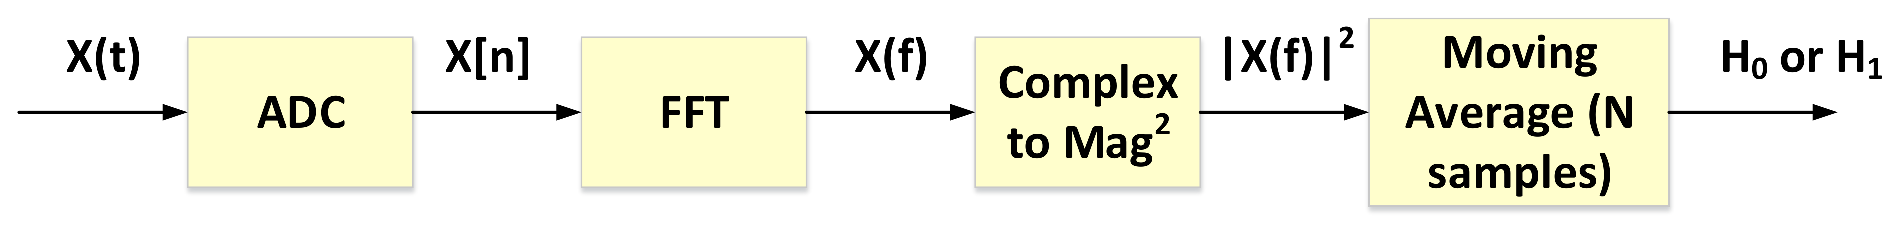
\includegraphics[width=\textwidth,keepaspectratio]{images/Gill/figs/energydet.eps}
    \caption{The block diagram describing the working of energy detection scheme.} 
\label{energydet}      
\end{figure}


The decision whether the signal is present or absent is decided by evaluating a local test statistic $L$ to see whether it is above or below certain fixed threshold $\tau$. 
The local test statistic $L$, which is the complex-magnitude squared of the FFT samples, is compared with $\tau$ using equation:

\begin{equation}
\label{eq:2}
	L = \sum_{n=1}^{M}{|y(n)|^2} = 
	\left\{
	\begin{aligned}
		<\tau,~\Hmat_0 \\
		>\tau,~\Hmat_1		
	\end{aligned}
	\right.
\end{equation}
where $|y(n)|^2$ is the energy of a specific FFT bin and n=1,2,3...M are the number of samples received.

The probability of false alarm $P_{fa}$ and probability of detection $P_d$ are given by:
\begin{equation}
\label{eq:3}
P_f = Q\Bigg(\dfrac{\tau-M(2\sigma_n^2)}{\sqrt{M}(2\sigma_n^2)}\Bigg),
\end{equation}

\begin{equation}
\label{eq:4}
~~~~~~~P_d = Q\Bigg(\dfrac{\tau-M(2\sigma_n^2)(1+\gamma)}{\sqrt{M(1+2\gamma)}(2\sigma_n^2)}\Bigg).
\end{equation}

\subsection{Cyclostationary Method}

There are lot of applications where it is required to perform the modulation recognition and signal classification. Communication signals can be more accurately described as statistical processes which repeats itself cyclically or periodically rather than a stationary process. Mathematically Cyclostationary feature detection scheme can be described by the equation~\cite{bookhtn1}:

\begin{figure}[ht!]
	\centering
	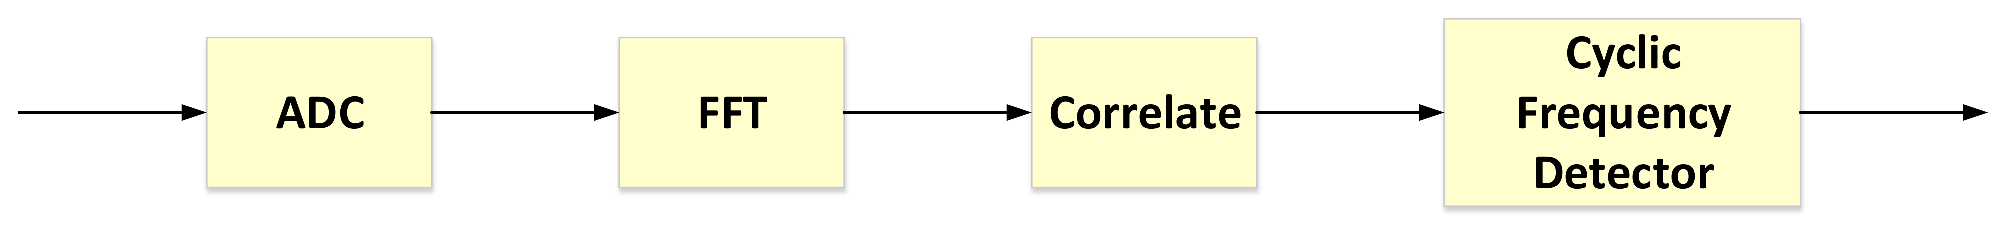
\includegraphics[width=\textwidth,keepaspectratio]{images/Gill/figs/cyclostationary.eps}
    \caption{The block diagram describing the working of cyclostationary feature detection scheme.} 
\label{cycl}      
\end{figure}

\begin{equation}
\label{eq:cyclo}
R_x(t,\tau) = E\Bigg\{x\bigg(t+\tau \bigg)x^*\bigg(t-\tau \bigg)\Bigg\} = \sum_{\{\alpha\}} R_x^{\alpha}(\tau)e^{j2\pi\alpha t}
\end{equation}

The Eq~.(\ref{eq:cyclo}) shows the autocorrelation of the observed signal $x(t)$ with periodicity $\tau$, $E\{.\}$ is the expectation operator, $\{\alpha\}$ is the set of Fourier components and $R_x^{\alpha}$ is the cyclic autocorrelation function (CAF) and is given by:

\begin{equation}
R_x^{\alpha} = \lim_{T\rightarrow \inf}\int_{-T/2}^{T/2} R_x(t,\tau)e^{-j2\pi\alpha t}
\end{equation}

Figure~\ref{cycl} shows the block diagram implementation of cyclostationary feature detection scheme where we correlate the frequency domain signal and then pass it to the cyclic frequency detection block and perform the signal classification.

\subsection{Matched Filter Detection}

In the matched filter detection method a known signal is correlated with an unknown signal captured from the available radio resource to detect the presence of pattern in the unknown signal. It is an optimal filter that projects the received signal in the direction of the pilot signal $x_p$~\cite{weidling2005framework}. The test statistic is given by:

\begin{equation}
T_{MD} = \sum_N y(n)x^*_p(n)
\end{equation}
The test statistic $T_{MD}$ is compared with a particular threshold to decide whether the signal is present or absent.The probability of detection $P_d$ and probability of false alarm $P_{fa}$ can be expressed as:
\begin{equation}
P_d = Q\bigg(\dfrac{\lambda-E}{\sqrt{E\sigma_{n,r}^2}}\bigg)
\end{equation}

\begin{equation}
P_{fa} = Q\bigg(\dfrac{\lambda}{\sqrt{E\sigma_{n,r}^2}}\bigg)
\end{equation}

where $E$ is the energy of the signal source, $\lambda$ is the detection threshold and $\sigma_{n,r}$ is the noise variance. The use of matched filter is very limited due to the requirement of apriori information which is not feasible in most cases. 

\section{Cognitive Radios}
Cognitive radio (CR)~\cite{cogjm} is a communication systems paradigm that focuses on employing highly agile, environmentally aware, intelligent wireless platforms in
order to autonomously select and configure device operating parameters based on the prevailing radio and network environmental conditions~\cite{bookhtn1}. In general the cognitive radio may be expected to look at parameters such as channel occupancy rate, available channels, bandwidth required for data transmission and the modulation types that may be used. It must also look at the regulatory requirements set by the Federal Communications Commission. In some instances a knowledge of geography and this may alter what it may be allowed to do. Software-defined radios (SDR) are mainly responsible for making cognitive radios used in wireless communications system a reality. Software radios provide a vast untapped potential to personalize services, and they make the process of modifying the radio characteristics extremely simple. 

The work is underway to determine the best possible methods of developing the cognitive radio communications system that can fulfill all its requirements. To facilitate the intelligent decision making capabilities in these cognitive radio systems, machine learning algorithms have been proposed in the literature~\cite{barker2008mission,haykin2005cognitive,newman2007cognitive,newman2008population} to automate the reconfiguration process. The Figure~\ref{cograd} describes the various building blocks of a cognitive radio system. The spectrum sensing is performed to estimate the spectrum holes in the band and after the analysis the decision strategy is prepared. The radio is configured with the new parameters based on the radio environment and the spectrum decision made.  

\begin{figure}[ht!]
	\centering
	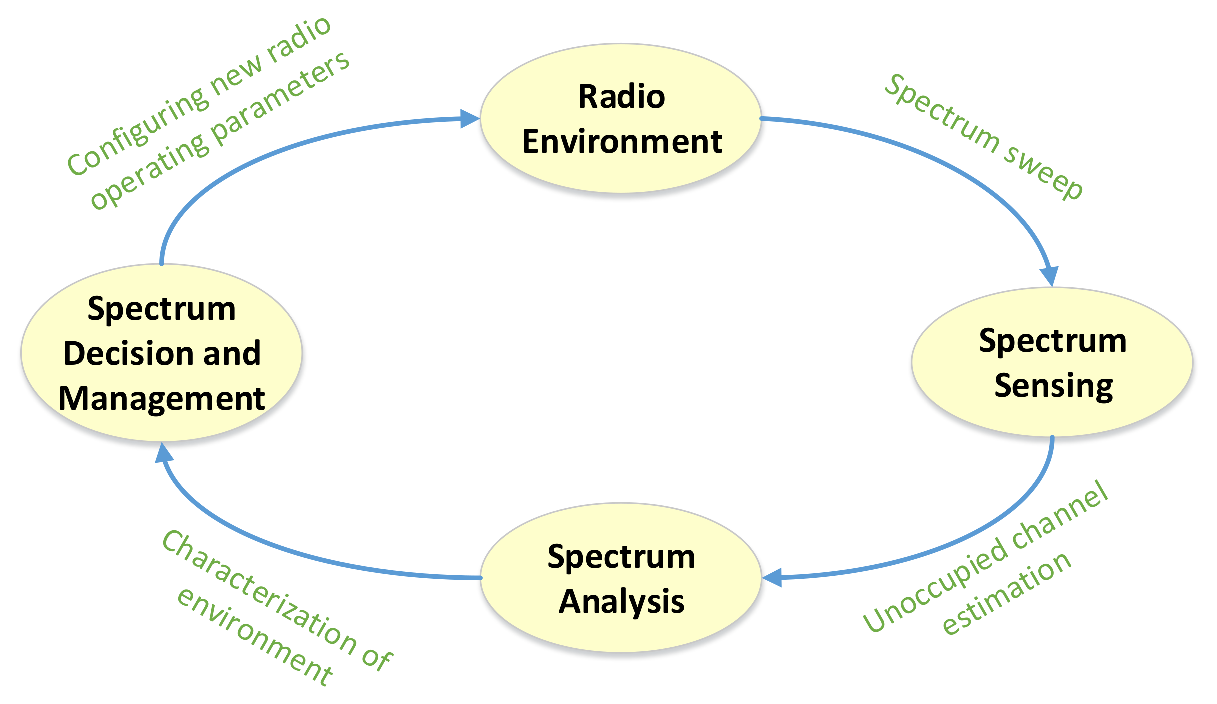
\includegraphics[width=\textwidth,keepaspectratio]{images/Gill/figs/cognitive_radio.eps}
    \caption{The block diagram explaining the basic parts of Cognitive Radio system. The operating parameters are configured based on the characterization of the wireless environment.} 
\label{cograd}      
\end{figure}

\section{CSS in Heterogeneous Networks}
In Heterogeneous CR network, each radio is equipped with different numbers of antennas, sampling rates and RF characteristics. In addition, each sensor node may experience distinct channel fading and suffer from different noise levels due to their respective locations and device performances, such as amplifier and ADC.  As a result, each node may have different sensing capabilities and reliability values. This is a universal and fundamental characteristic of a heterogeneous CR network which requires robust algorithms to achieve high accuracy in signal source detection for estimating the presence of a primary user\cite{arhtn13}. In this thesis, we investigate the cooperative spectrum sensing in heterogeneous networks with a centralized FC, a transmitter acting as a signal source and four sensor nodes. As explained earlier we are using energy detection as one of the spectrum sensing technique since it possesses a very low implementation complexity~\cite{arhtn4}. The energy detection scheme detects the presence or absence of a signal source based on its intercepted energy signature. If the energy of the signal is higher than a certain threshold, this indicates that the channel is occupied. 


In cooperative spectrum sensing, each sensor node transmits the local sensing data to the fusion center for signal source detection. The local sensing data has to be quantized, thus yielding quantization errors. To minimize the quantization error in local test statistic $L$ and to reduce the effect of noise variance, the energy of the received signal $y(n)$ is normalized\cite{arhtn13}. The local test statistic $L$ for the $r^{th}$ sensor node is given as:
\begin{equation}
	\label{eq:5}
	L_r = \dfrac{1}{M_r\sigma_{n,r}^2}\sum_{r=1}^{M_r}|y(n)|^2
\end{equation}
where $M_r$ is the number of samples used to estimate the power of the signal source in the node,  $\sigma_{n,r}$ is the noise power variance.

In Eq~(\ref{eq:1}) $s(n)$ is considered as a deterministic signal and $w(n)$ is a Gaussian random variable with a variance of $\sigma_n^2$. Based on CLT, $L_r$ will have a following distribution~\cite{inphtn7}:

\begin{equation}
	\label{eq:6}
	L_r = 
	\left\{
	\begin{aligned}
		& N(1,\dfrac{1}{M_r}),~~~~~~~~~~~~\Hmat_0 \\
		& N(\gamma_r+1,\dfrac{1+2\gamma_r}{M_r}),~\Hmat_1		
	\end{aligned}
	\right.
\end{equation}
where $\gamma_r$ is the received SNR of the $r^{th}$ SU. The local decision statistic $L_r$ is quantized before transmission due to the bandwidth constraint, and this can lead to quantization errors. The values of $L_r$ received by FC can be modeled as:
\begin{equation}
	\label{eq:7}
	 \beta_r = L_r + w_{q,r},
\end{equation}
where $\beta_r$ is the decision statistic received by the FC and $w_q$ is the noise added to the signal due to fading and quantization error. In \cite{arhtn14}, the $w_q$ is modeled as a Gaussian noise with zero mean and $\sigma_q^2$ variance.

\section{Software Defined Radios}
We have already explained about the cooperative spectrum sensing in heterogeneous networks, now in this section we will look at the platform for testing the CSS algorithms. The platform which we use is a new hardware frontier called Software-Defined Radio (SDR) and is discussed in details.

\begin{figure}[ht!]
	\centering
	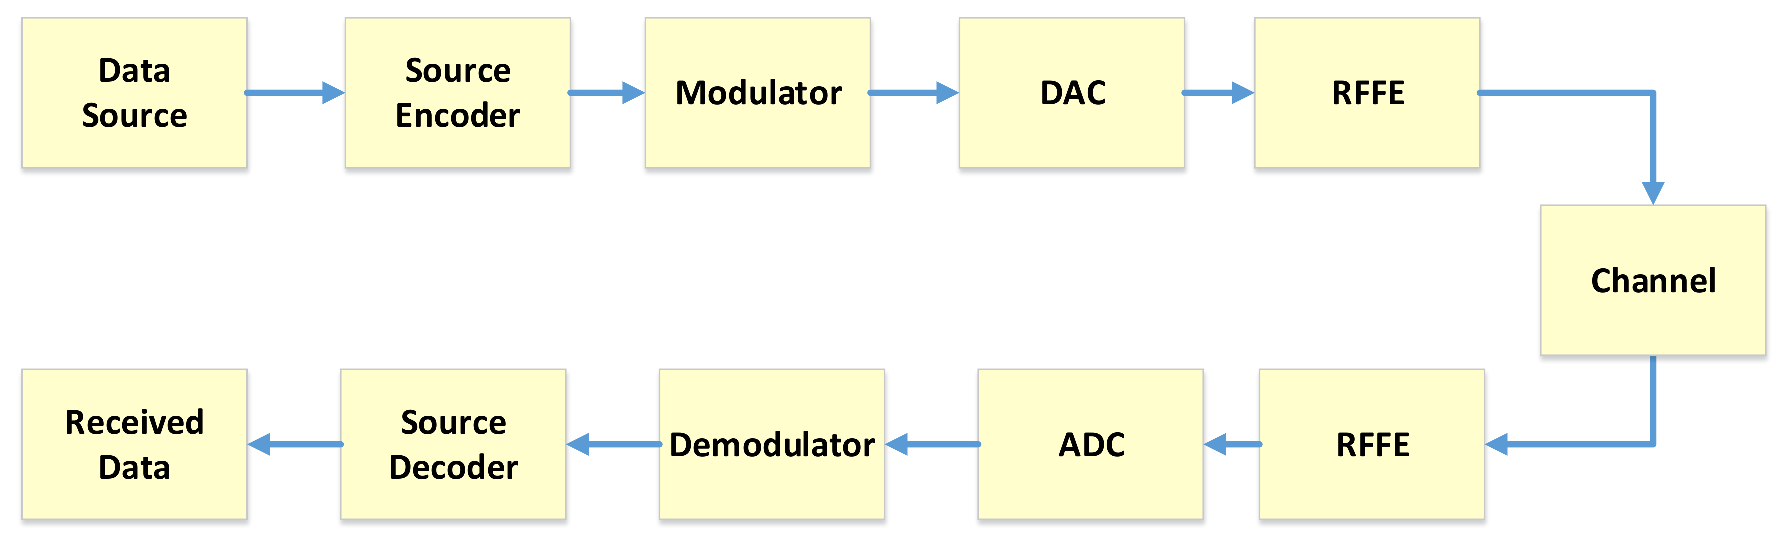
\includegraphics[width=\textwidth,keepaspectratio]{images/Gill/figs/softwaredefinedradio.eps}
    \caption{Software defined radio pushes all the adaptive elements and data manipulation operation into software. The goal of SDR is to provide or define all of the radio operation in software.} 
\label{sdr}      
\end{figure}

There has been a huge shift in the definition of a Software-Defined Radio and it has a lot to do with the question of where the hardware ends and software begins. Dr. J. Mitola III coined the Software Defined Radio which he described as a of digital signal processing (DSP) primitives, a meta-level system for combining the primitives into communication system (Tx, channel model, Rx, etc.), functions and a set of target processors on which the software radio is hosted for real-time communications~\cite{267870}. Dr. J. Mitola explains in the thesis how software provides the flexibility which using hardware alone can never be achieved. And as time progresses SDR would become more dominant and close to ideal Cognitive Radio system.

The SDR technology existed since the 1970s but the key milestone in the advancement of SDR technology took place in early 1990s with the U.S. military initiative called SpeakEasy I/II. The SpeakEasy project was implemented to use programmable processing to emulate more than ten existing military radios, operating in frequency bands between 2 MHz and 2 GHz~\cite{392998}. With SpeakEasy the operator could talk to ten radios operating under different standards with any hardware modifications. With all these features, unfortunately there were some shortcomings which left much to be desired. The device was large enough to fit on the back of a pickup truck~\cite{392998} which is good for ground station but not if the mobility is an important factor. And in 1992 the field programmable gate arrays (FPGA) were not computationally efficient, hence required large time to change their operating characteristics. The two software-defined radios we used in the thesis are Universal Software Radio Peripheral (USRP N210) and RTL-SDR R2832U. In the subsequent subsections we discuss the two SDRs in detail.

\subsection{USRP N210 and RTL-SDR}

The Universal Software Radio Peripheral (USRP) N210 has a very different RF characteristics compared to RTL-SDR hence modeling an ideal heterogeneous network. The USRP N210 provides a very high bandwidth, dynamic range processing capability. The product architecture includes a Xilinx Spartan 3A-DSP 3400 FPGA~\cite{xilinx}, 100 MS/s dual ADC, 400 MS/s dual DAC and gigabit ethernet connectivity to stream data to and from host processors. A modular design allows the USRP N210 to operate from DC to 6 GHz, while an expansion port allows multiple USRP N210 series devices to be synchronized and used in a MIMO configuration. An optional GPSDO module can also be used to discipline the USRP N210 reference clock to within 0.01 ppm of the worldwide GPS standard. The USRP N210 can stream up to 50 MS/s to and from host applications. Users can implement custom functions in the FPGA fabric, or in the on-board 32-bit RISC softcore. The USRP N210 provides a larger FPGA than the USRP N200 for applications demanding additional logic, memory and DSP resources. The FPGA also offers the potential to process up to 100 MS/s in both the transmit and receive directions. The FPGA firmware can be reloaded through the Gigabit Ethernet interface~\cite{usrp}.

RTL-SDR is a very cheap software defined radio that uses a DVB-T TV tuner dongle based on the RTL2832U chipset. With the combined efforts of Antti Palosaari, Eric Fry and Osmocom it was found that the signal I/Q data could be accessed directly, which allowed the DVB-T TV tuner to be converted into a wideband software defined radio via a new software driver. Essentially, this means that a cheap \$20 TV tuner USB dongle with the RTL2832U chip can be used as a computer based radio scanner. This sort of scanner capability would have cost hundreds or even thousands of dollars just a few years ago. The RTL-SDR is also often referred to as RTL2832U, DVB-T SDR, RTL dongle or the “\$20 Software Defined Radio”.

\subsection{GNU Radio and MATLAB}
We have used GNU Radio~\cite{gnradio} and MATLAB software in the thesis to implement the cooperative spectrum sensing for hard decision and soft decision schemes. GNU Radio  
is an open source development toolkit that provides re-configurable signal processing blocks to implement and test out software-defined radios and signal processing systems. GNU Radio allows for SDR developers to develop unique signal processing blocks and SDR systems. GNU Radio was started in 2001, originally forked from the SpectrumWare project developed at the Massachusetts Institute of Technology. Since 2001, the code base has undergone massive changes, containing almost no code from the original SpectrumWare project~\cite{bose1999virtual}. Physically the code consist of three languages Python, C++, and SWIG. Python provides the overarching control of the system or program, while C++ provides the actual signal processing blocks and mathematics. SWIG is a wrapper for C++ which allows Python to dynamically wrap around C++ and control or compile with it. A diagram below better illustrates this architecture. It is also important to mention that there as significant paradigm shifts in the community, pushing more and more code to Python rather than C++, due to its easier programming syntax and structure~\cite{collins2013implementation}.

\begin{figure}[ht!]
	\centering
	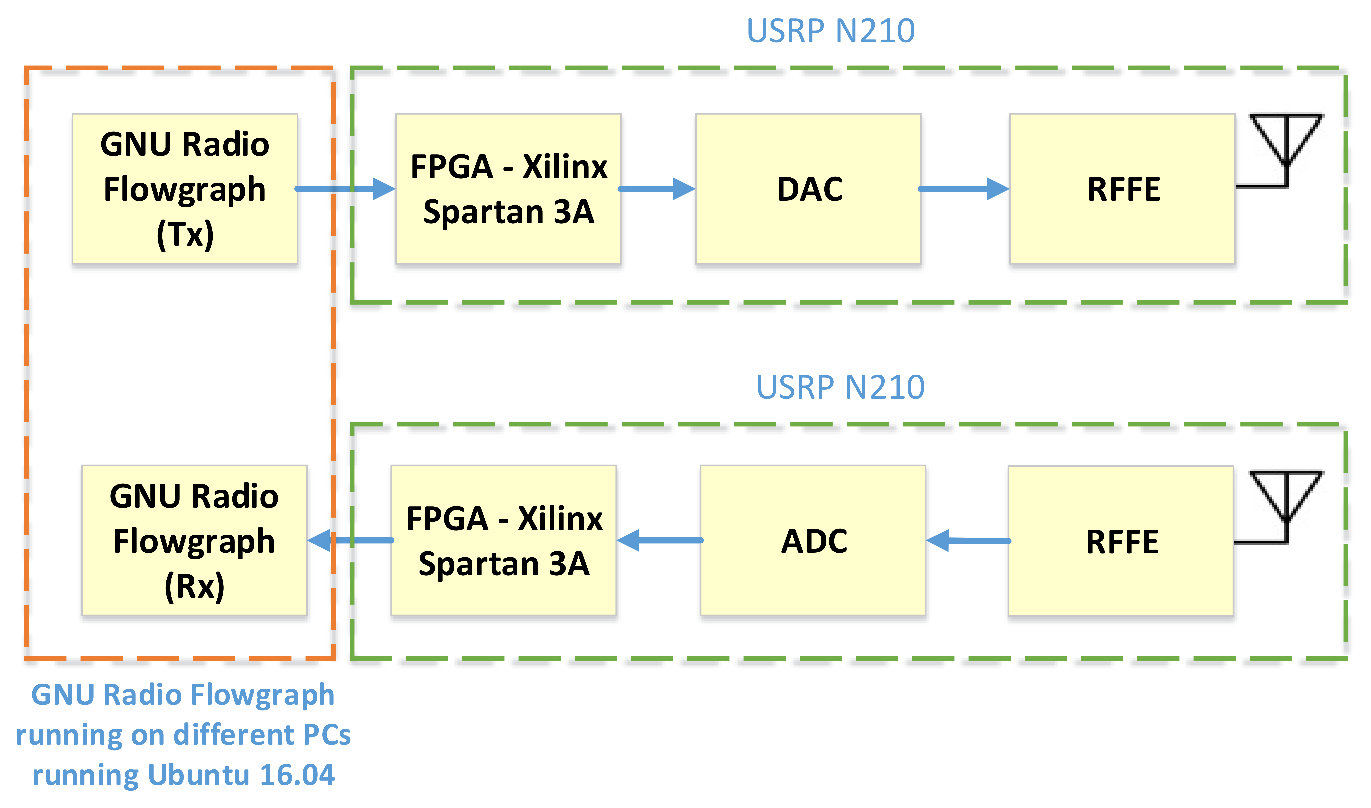
\includegraphics[width=\textwidth,keepaspectratio]{images/Gill/figs/gnuradio.eps}
    \caption{GNURadio and Software-Defined Radio} 
\label{gnuradio}      
\end{figure}

The GNU Radio software provides the framework and tools to build and run software radio or just general signal-processing applications. The GNU Radio applications themselves are generally known as "flowgraphs", which are a series of signal processing blocks connected together, thus describing a data flow. GNU Radio provides a very structured framework of flow design. Data processing segments are extremely self contained to minimize error propagation during system debugging. Since the software is open-source full access to all code is provide, giving low-level access to all operation within GNU Radio. Much of the actions have been abstracted to the limited knowledge of the lower layers, but if specific actions are required for an application then serious depth or knowledge is needed about the overall project’s structure, which is quite overloading.

MATLAB~\cite{matlab} is an extremely well known engineering, mathematical, biological, and financial software suite. MATLAB provide massive data leverage and advanced communication system models and algorithm for significant data processing.

\section{Summary}
In this chapter we discussed the heterogeneous cooperative spectrum sensing and examined various spectrum sensing techniques. We also discussed cognitive radios, CSS in heterogeneous networks, software-defined radios in details. We discuss three popular spectrum sensing techniques in details and, also outlined software-defined radios USRP N210 and RTL-SDR and their RF characteristics. Finally we described GNU Radio and MATLAB: software tools used in the thesis to implement the CSS test-bed. 


%% Heterogeneous CSS Implementation..
\chapter{Proposed LTE-R Test-bed Implementation and Results}
\label{chapter4}

This chapter provides background information on LTE proposed for high-speed railway communication system. It outlines the architecture for LTE-R leveraging the existing LTE network for high speed railway networks. For uniform coverage inside a tunnel environment, leaky coaxial cables (LCX) has been proposed for efficient communication. We explain LCX cables in details in the following chapter especially for tunnel environment. The severe channel impairments inside a tunnel are also discussed with special attention to high Doppler shift cause due to high velocities of trains and harsh multipath fading environment. Finally, the proposed two-ray propagation channel model is discussed and dynamic K-factor is derived.

\section{LTE-R Testbed in Matlab}

We have implemented the simulation testbed in MATLAB, consisting of a transmitter, a channel and a receiver. The K-factor values for the channel model are obtained from Eq.(\ref{kfactor}) and are used to generate a time-series BER curve for different modulation schemes used in LTE-R. The values used for the electrical material properties for tunnel walls~\cite{lter17} and its
specifications are given in Table~\ref{tablelter}. The relative permittivity for the tunnel walls is taken as $\varepsilon_r = 5$ and $\sigma$ is set to 0.1. The simulation is conducted for velocity of $v (Km/h) = $ 300, 400 and 500 Km/h. Since the frequency band allocation for LTE-R will most probably be from 2--6 GHz, hence the $f_c$ values chose are 2, 3 and 5 GHz. The height of the receiver is assumed to be around the length of the train and height of tunnel is chosen as the size of the leaky coaxial cable.

\begin{table*}[t!]
\centering
\caption{Tunnel and Tx/Rx Characteristics}
\begin{tabular}{c  c  c }
   & Dimensions & Simulation Parameters\\\hline
Tunnel & Width = 8.6 m, Height = 7.3 m & $\varepsilon_r = 5$, $\sigma = 0.1~\textrm{Sm}^{-1}$\\\hline
Leaky Feeder Cable (Tx) & Height = 6.1 m & $f_c$ (GHz) = 2, 3, 5\\\hline
Train (Rx) & Height = 4.2 m &  v (km/h) = 300, 400, 500\\
\hline
\end{tabular}
\label{tablelter}
\end{table*}

\begin{figure}[!ht]
\label{finalblock}
\centering
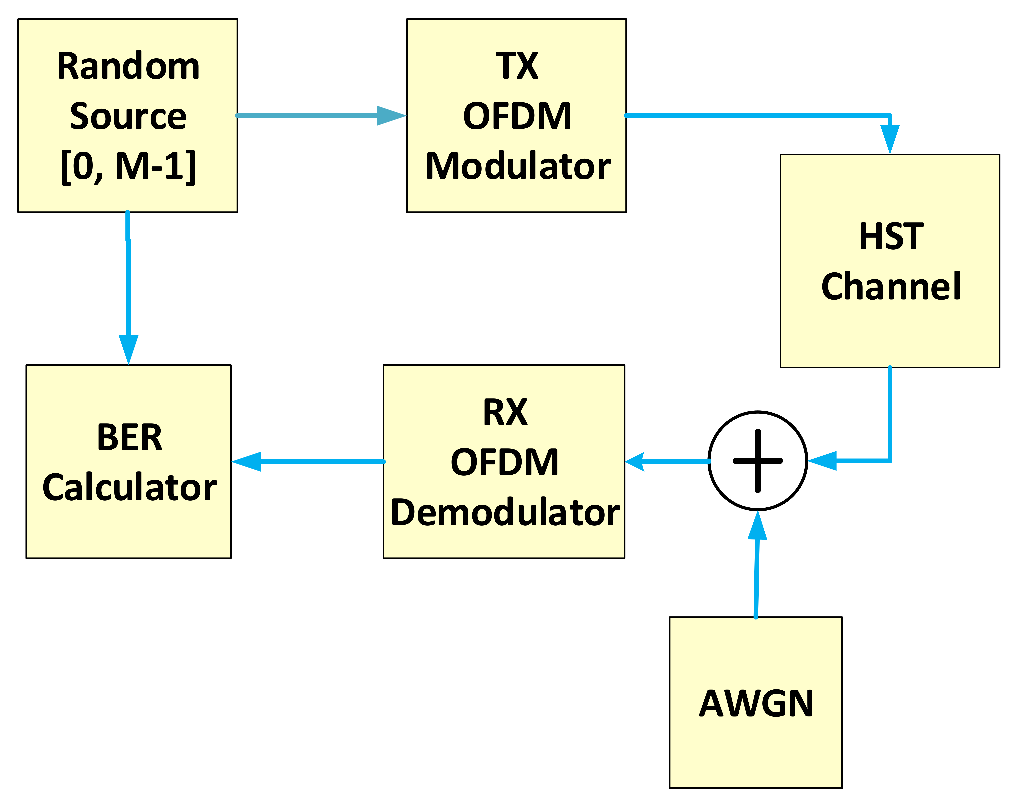
\includegraphics[width=\textwidth,height=8cm,keepaspectratio]{images/Gill/lte_figs/finalblock.eps} 
\caption{Block diagram of a communication system through a HST channel using QPSK, 16-QAM and 64-QAM.}
\end{figure}

Figure~\ref{finalblock} shows the block diagram of the simulation test-bed used for the performance analysis of LTE-R. The random source block generate the symbol between 0 and M-1, where M = 4,16,64 for QPSK, 16QAM and 64QAM respectively. The data is then modulated with specific modulation type and then pass through the proposed HST channel model. The additive white gaussian noise is added after applying the channel coefficients to the signal data. We then demodulate the data packets and pass it to the ber calculator object which then computes the bit-error rate. The simulations are run for SNR values ranging from 0--20 dB and plots are generated for all three modulation schemes.

\section{HST LTE-R in a Tunnel}
Using LTE System Toolbox provided by MATLAB we generated Figure~\ref{lteofdma} which shows the received resource grid without equalization. The frame worth of data was modulated with QPSK, 16QAM and 64QAM for equal number of subcarriers and mapped to symbol in a subframe. We generate ten subframes individually and create one frame after merging all subframes. The frame is passed through our proposed high speed train channel model, with additive white gaussian noise added. We can see that without equalization the received resourced grid has lot of errrors and will lead to numerous retransmissions.

\begin{figure}[!ht]
\label{lteofdma}
\centering
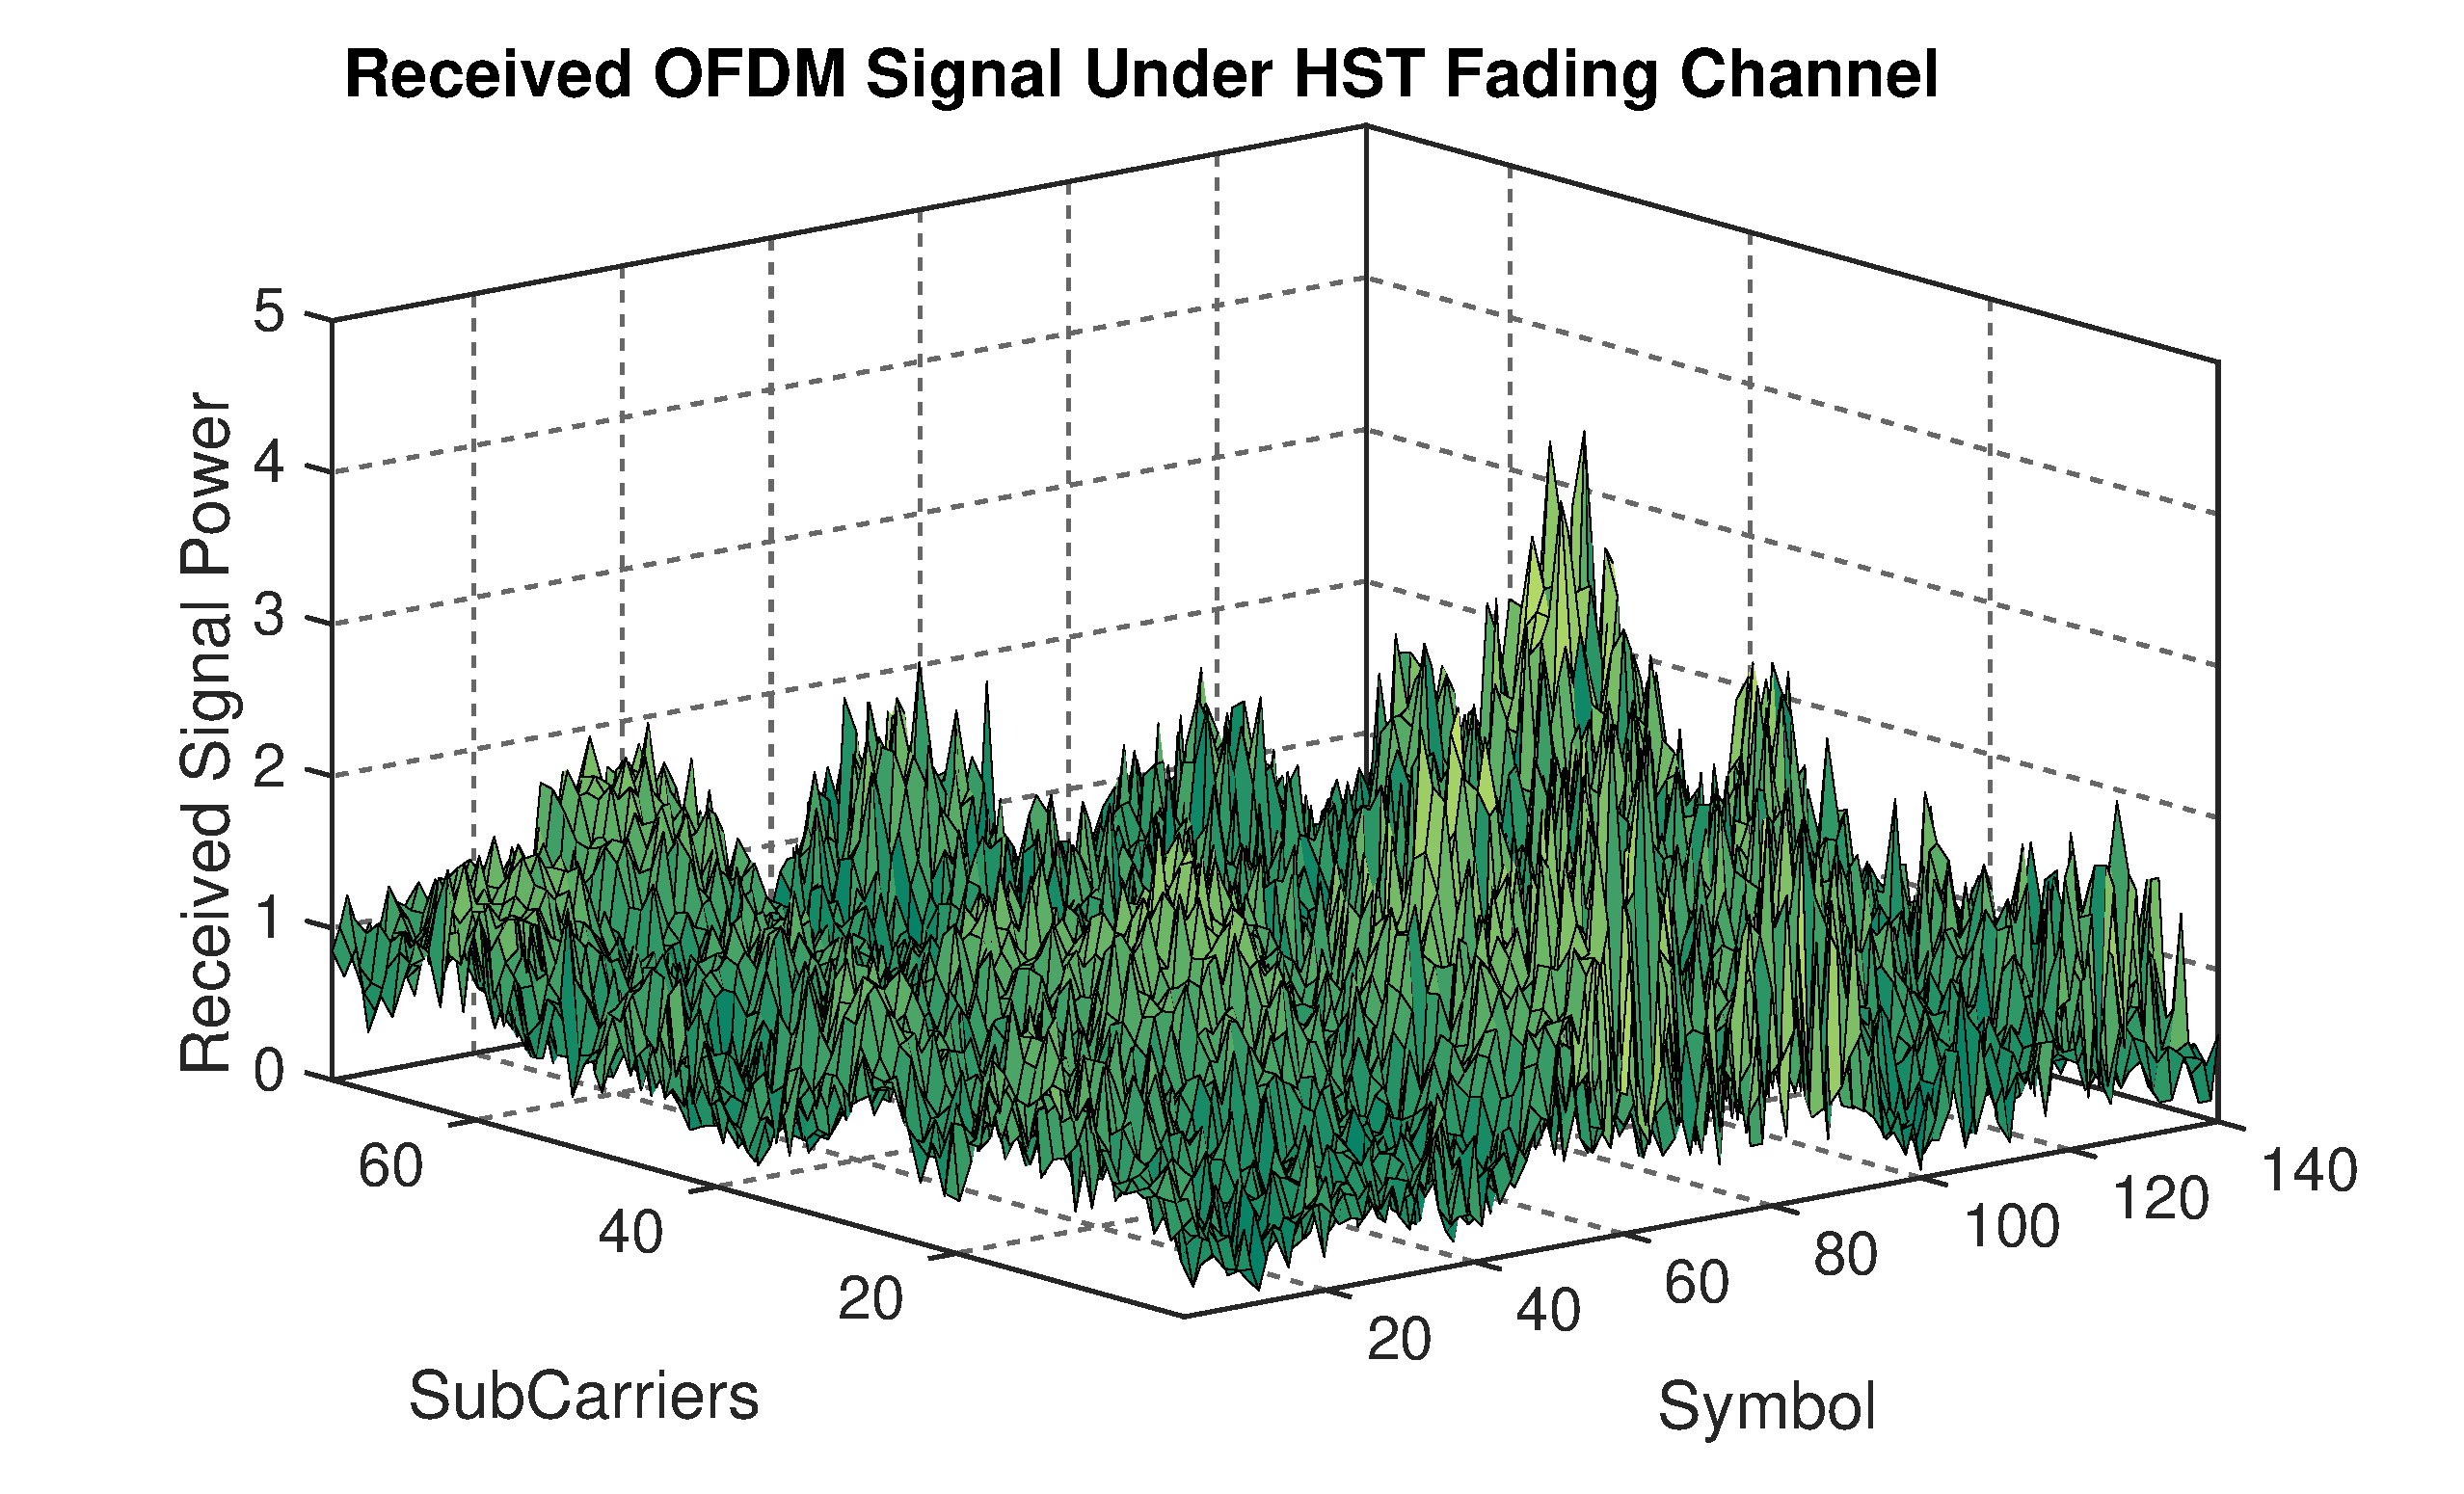
\includegraphics[width=\textwidth,keepaspectratio]{images/Gill/lte_figs/receivedsignal.eps} 
\caption{Received LTE-R OFDM signal under HST Ricean Fading Environment. }
\end{figure}

\subsection{K-factor in a Tunnel}
In Figure~\ref{kfactorber}, we calculated the K-factor for the HST inside a tunnel with velocity $v$ = 500 km/h for different center frequencies. It shows the variation of the Rician K-factor with the distance between the transmitter and receiver as the train is moving along the tunnel. We computed the K-factor for a leaky cable with periodic slots separated by distance d in fixed time-steps. The plot shows that the K-factor varies significantly over a short distances. Therefore, assuming a single K-factor for the channel model is not accurate, we use time-series K-factor to do our channel modeling.

\begin{figure}[!ht]
\label{kfactor}
\centering
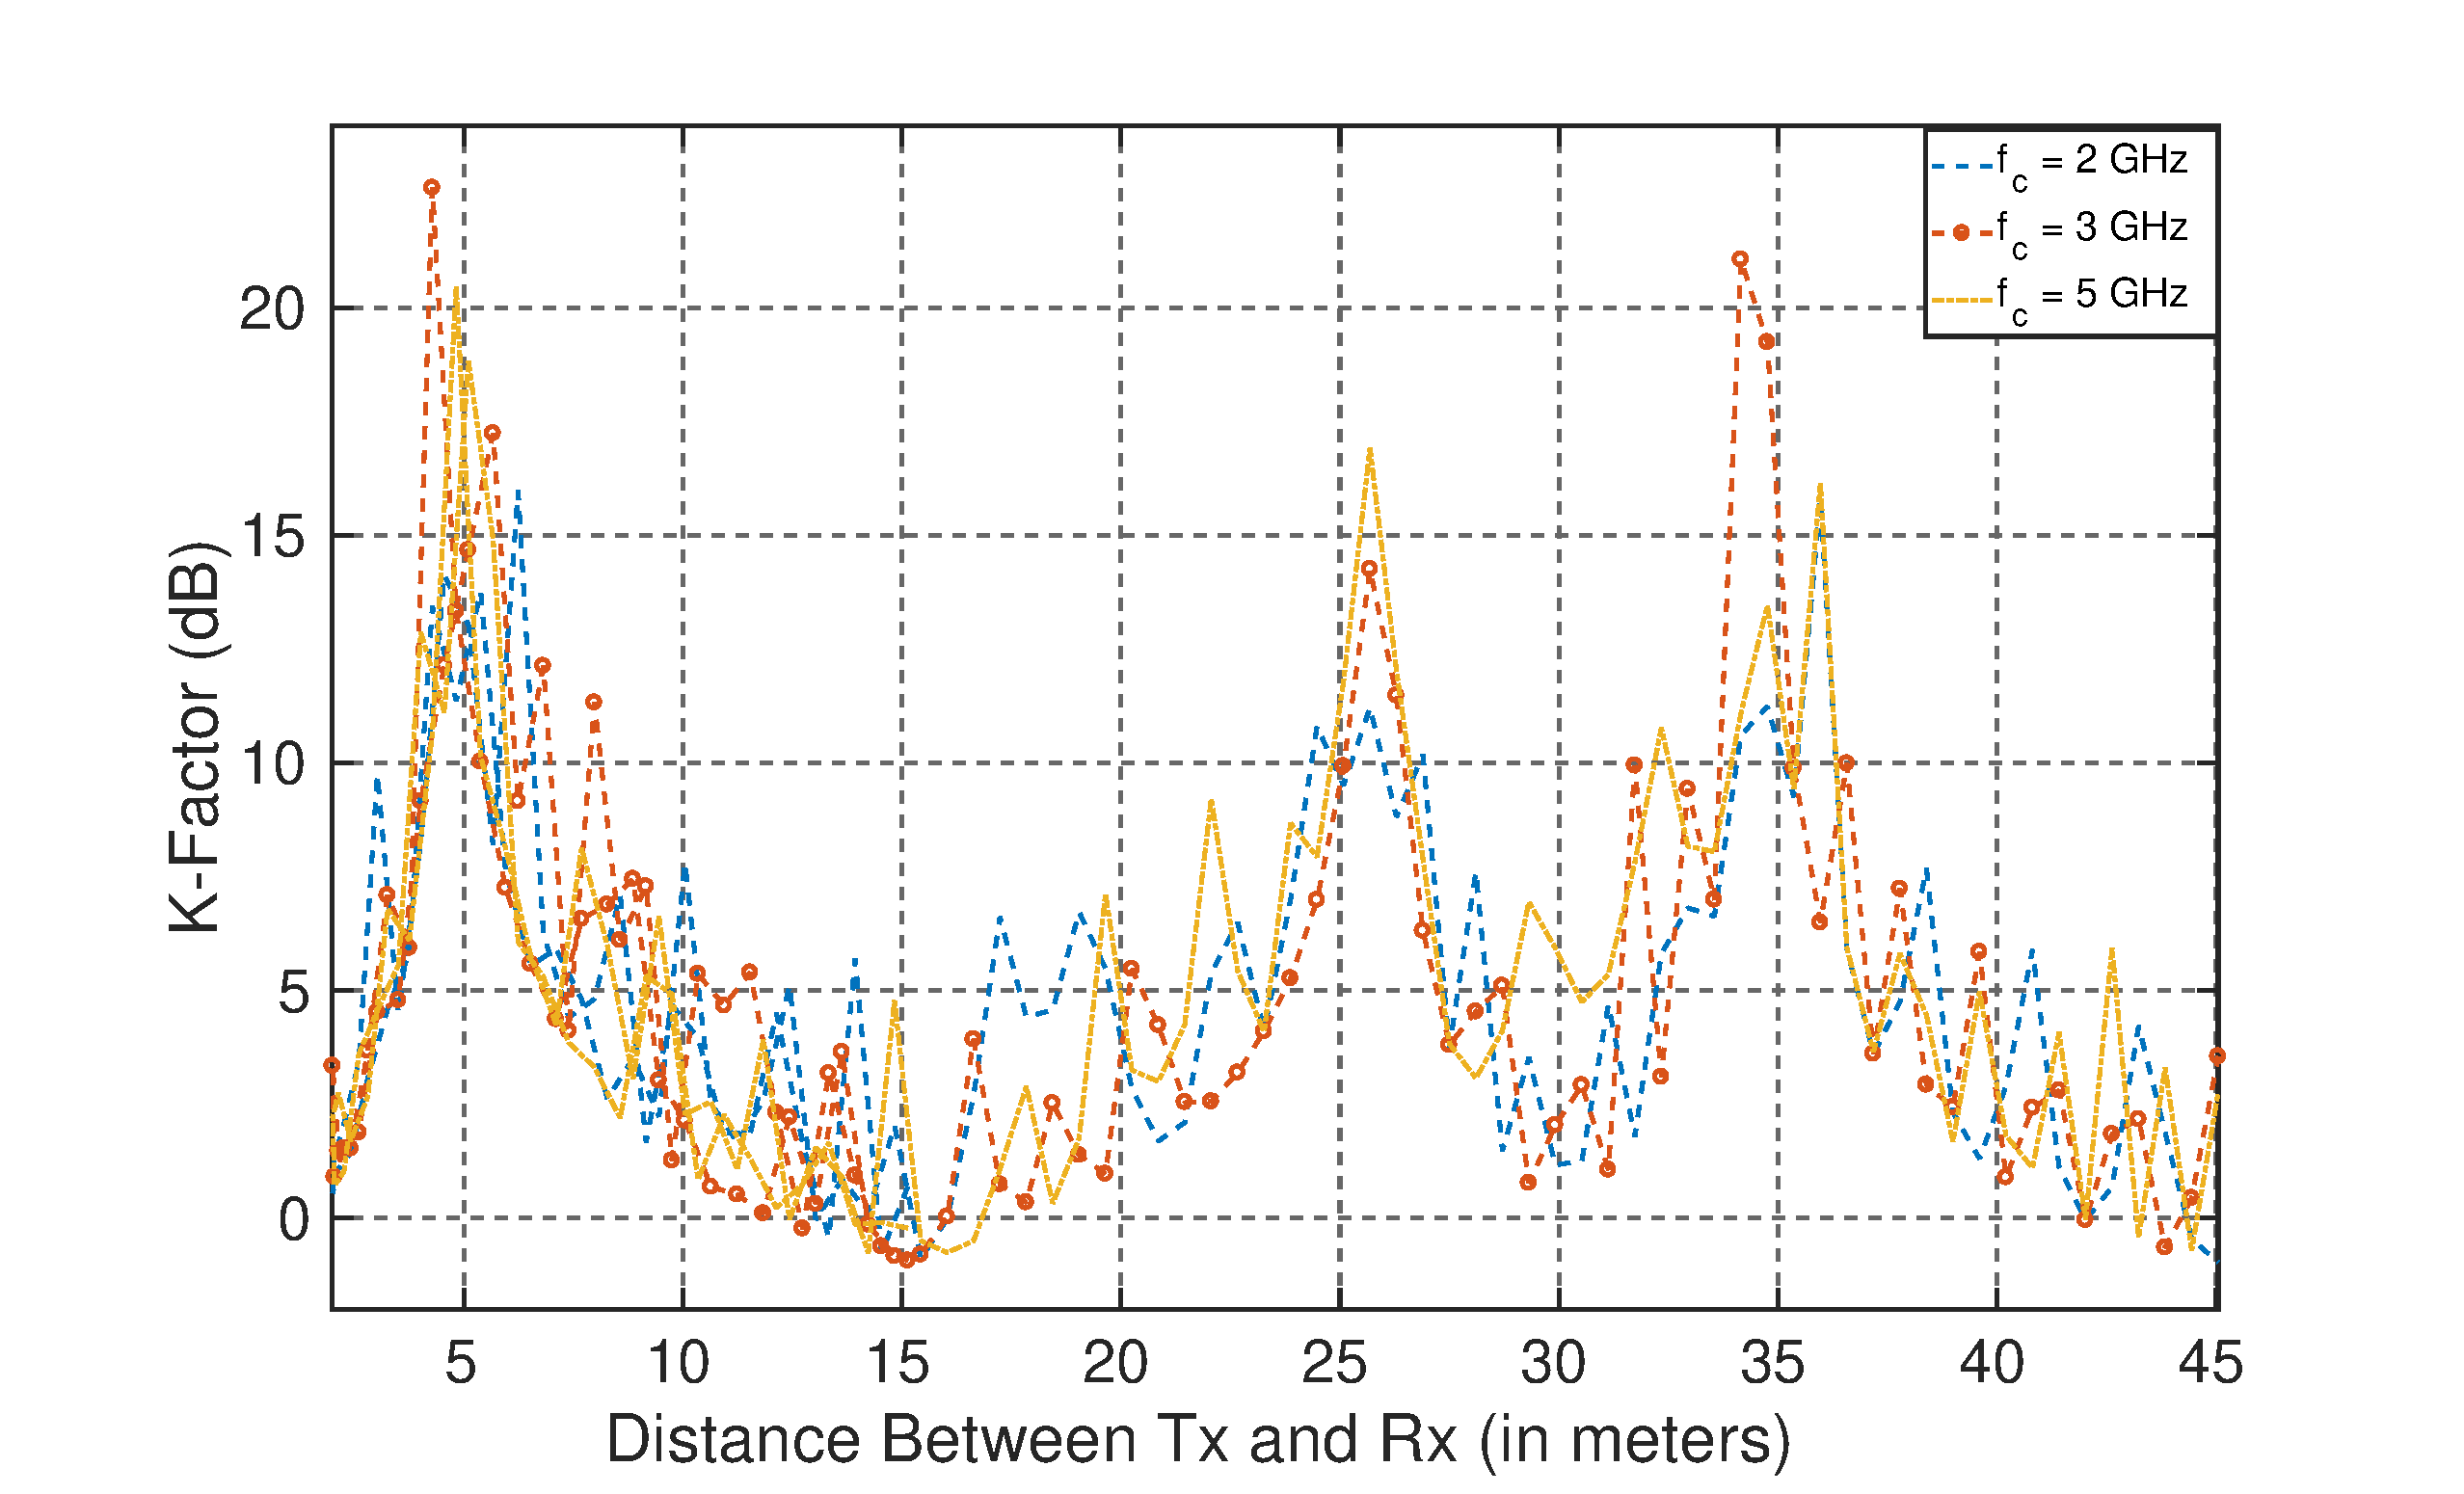
\includegraphics[width=\textwidth,keepaspectratio,height=8cm]{images/Gill/lte_figs/kfactordist.eps} 
\caption{K-factor versus $D_{LOS}$ for different center frequencies $f_c$ = 2, 3 and 5 GHz.}
\end{figure}

\subsection{BER Performance}
To show the impact of varying K-factor on the channel, we computed the BER curve for different modulation schemes of LTE-R with different K-factors. Fig.~\ref{fig:qpsk} shows the BER versus SNR performance for QPSK modulation for different K-factors of the tunnel channel model. The figure clearly demonstrates for higher K-factor we have a better performance while performance degrades as K-factor goes low. Fig.\ref{fig:qam16} shows the $E_b/N_0$ versus BER for 16-QAM and as we can see the BER is higher compared to QPSK. Fig.~\ref{fig:qam64} shows the $E_b/N_0$ versus BER for 64-QAM for different K-factors. And finally we compare all the modulation schemes for the best and worst K-factor in Fig.~\ref{fig:qamall}.

\begin{figure*}[t!]
  \begin{center}
  \subfloat[OFDM-QPSK]
  {\label{fig:qpsk}
  \includegraphics[width=0.46\textwidth]{images/Gill/lte_figs/qpskricean.eps}
  }\hspace{1mm}
   \subfloat[OFDM-16QAM]{\label{fig:qam16}\includegraphics[width=0.46\textwidth]{images/Gill/lte_figs/16qamricean.eps}}\hspace{1mm}
  \subfloat[OFDM-64QAM]{\label{fig:qam64}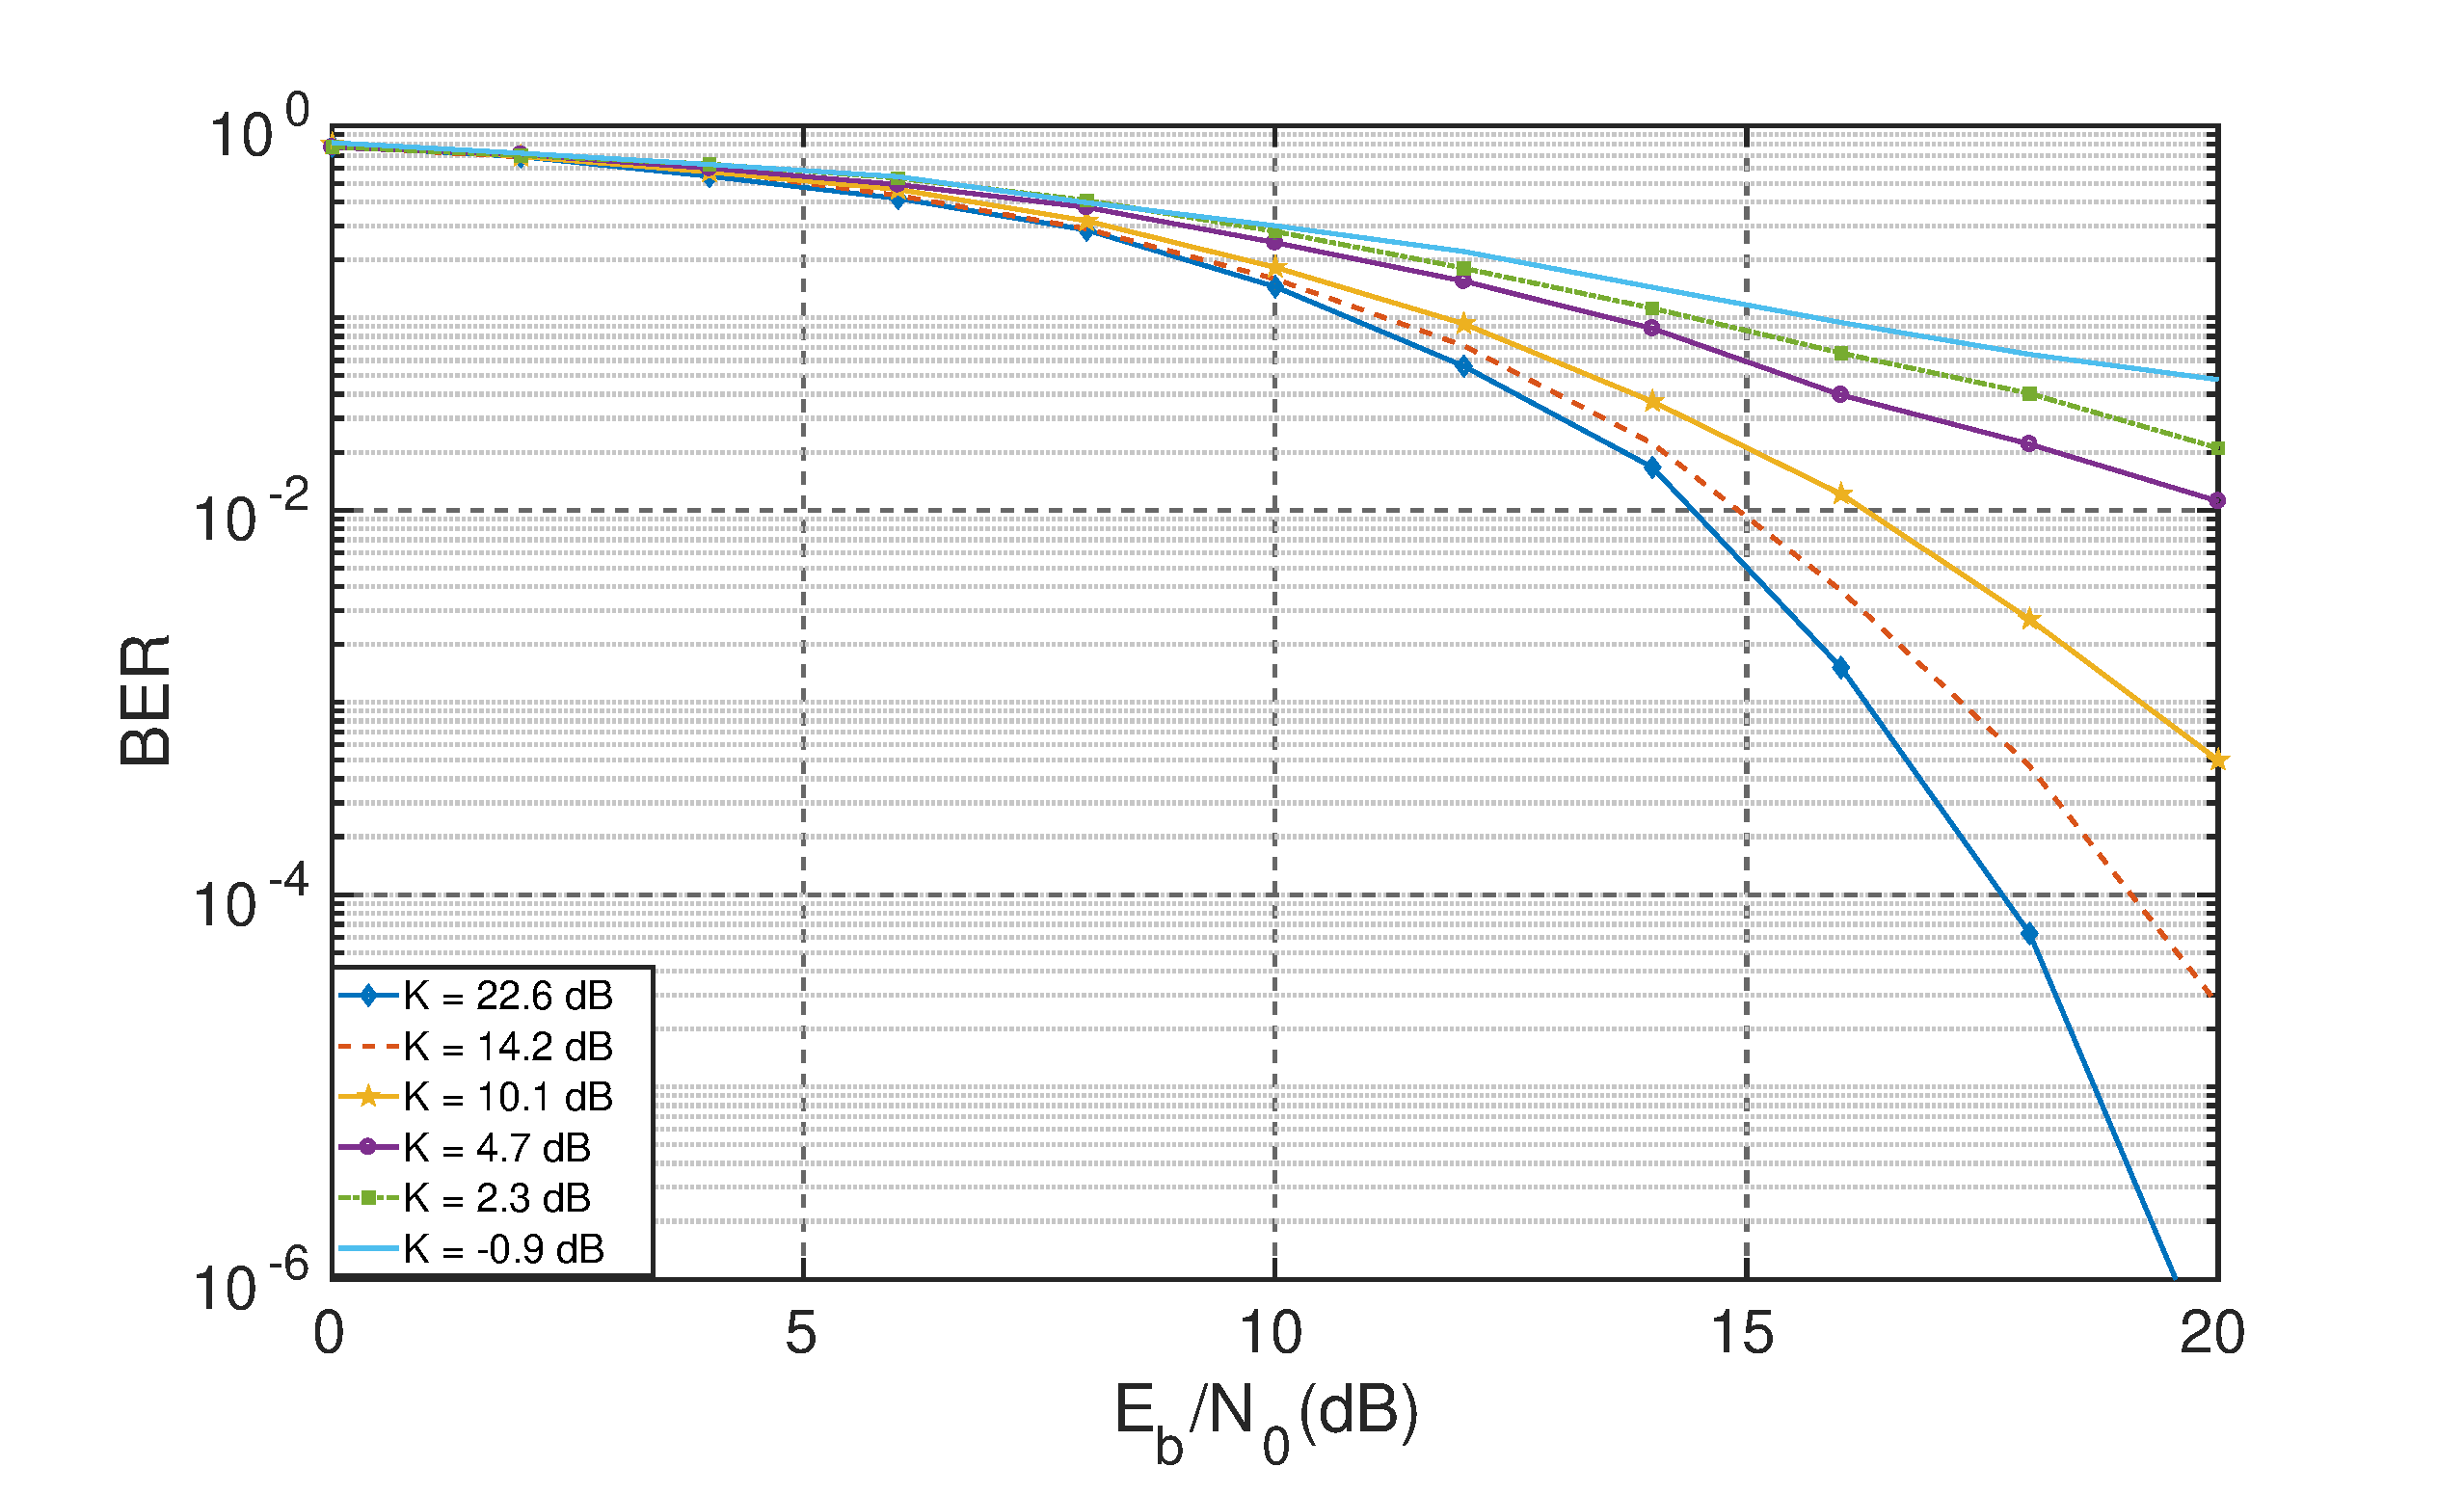
\includegraphics[width=0.46\textwidth]{images/Gill/lte_figs/64qamricean.eps}}\hspace{1mm}
   \subfloat[OFDM-MQAM]{\label{fig:qamall}\includegraphics[width=0.46\textwidth]{images/Gill/lte_figs/mqamricean.eps}}\hspace{1mm}
     \caption{Comparison of $E_b/N_0$ verus BER for LTE-R OFDM modulation with different $K$-factors. The first three sub-figures shows the $E_b/N_0$ versus BER for individual modulation schemes employed in LTE-R and in last plot we compare all the modulation schemes for different $K$-factors.} 
\label{fig:modulation}      
   \end{center}
\end{figure*}

In Fig.~\ref{kfactorber} we calculate the BER performance for a high speed train in discrete time-steps. As the train moves towards
the LCX slot the SNR goes high and the SNR decreases as the train moves away. This trend can be seen in the plot, as we move towards the slot the BER curve decreases and it starts increases once we move. It is important to consider here that due to the varying nature of K-factor the BER curve also varies significantly. Hence, by considering the time-varying nature of K-factor we can have a better performance analysis.

\begin{figure}[!ht]
\label{kfactorber}
\centering
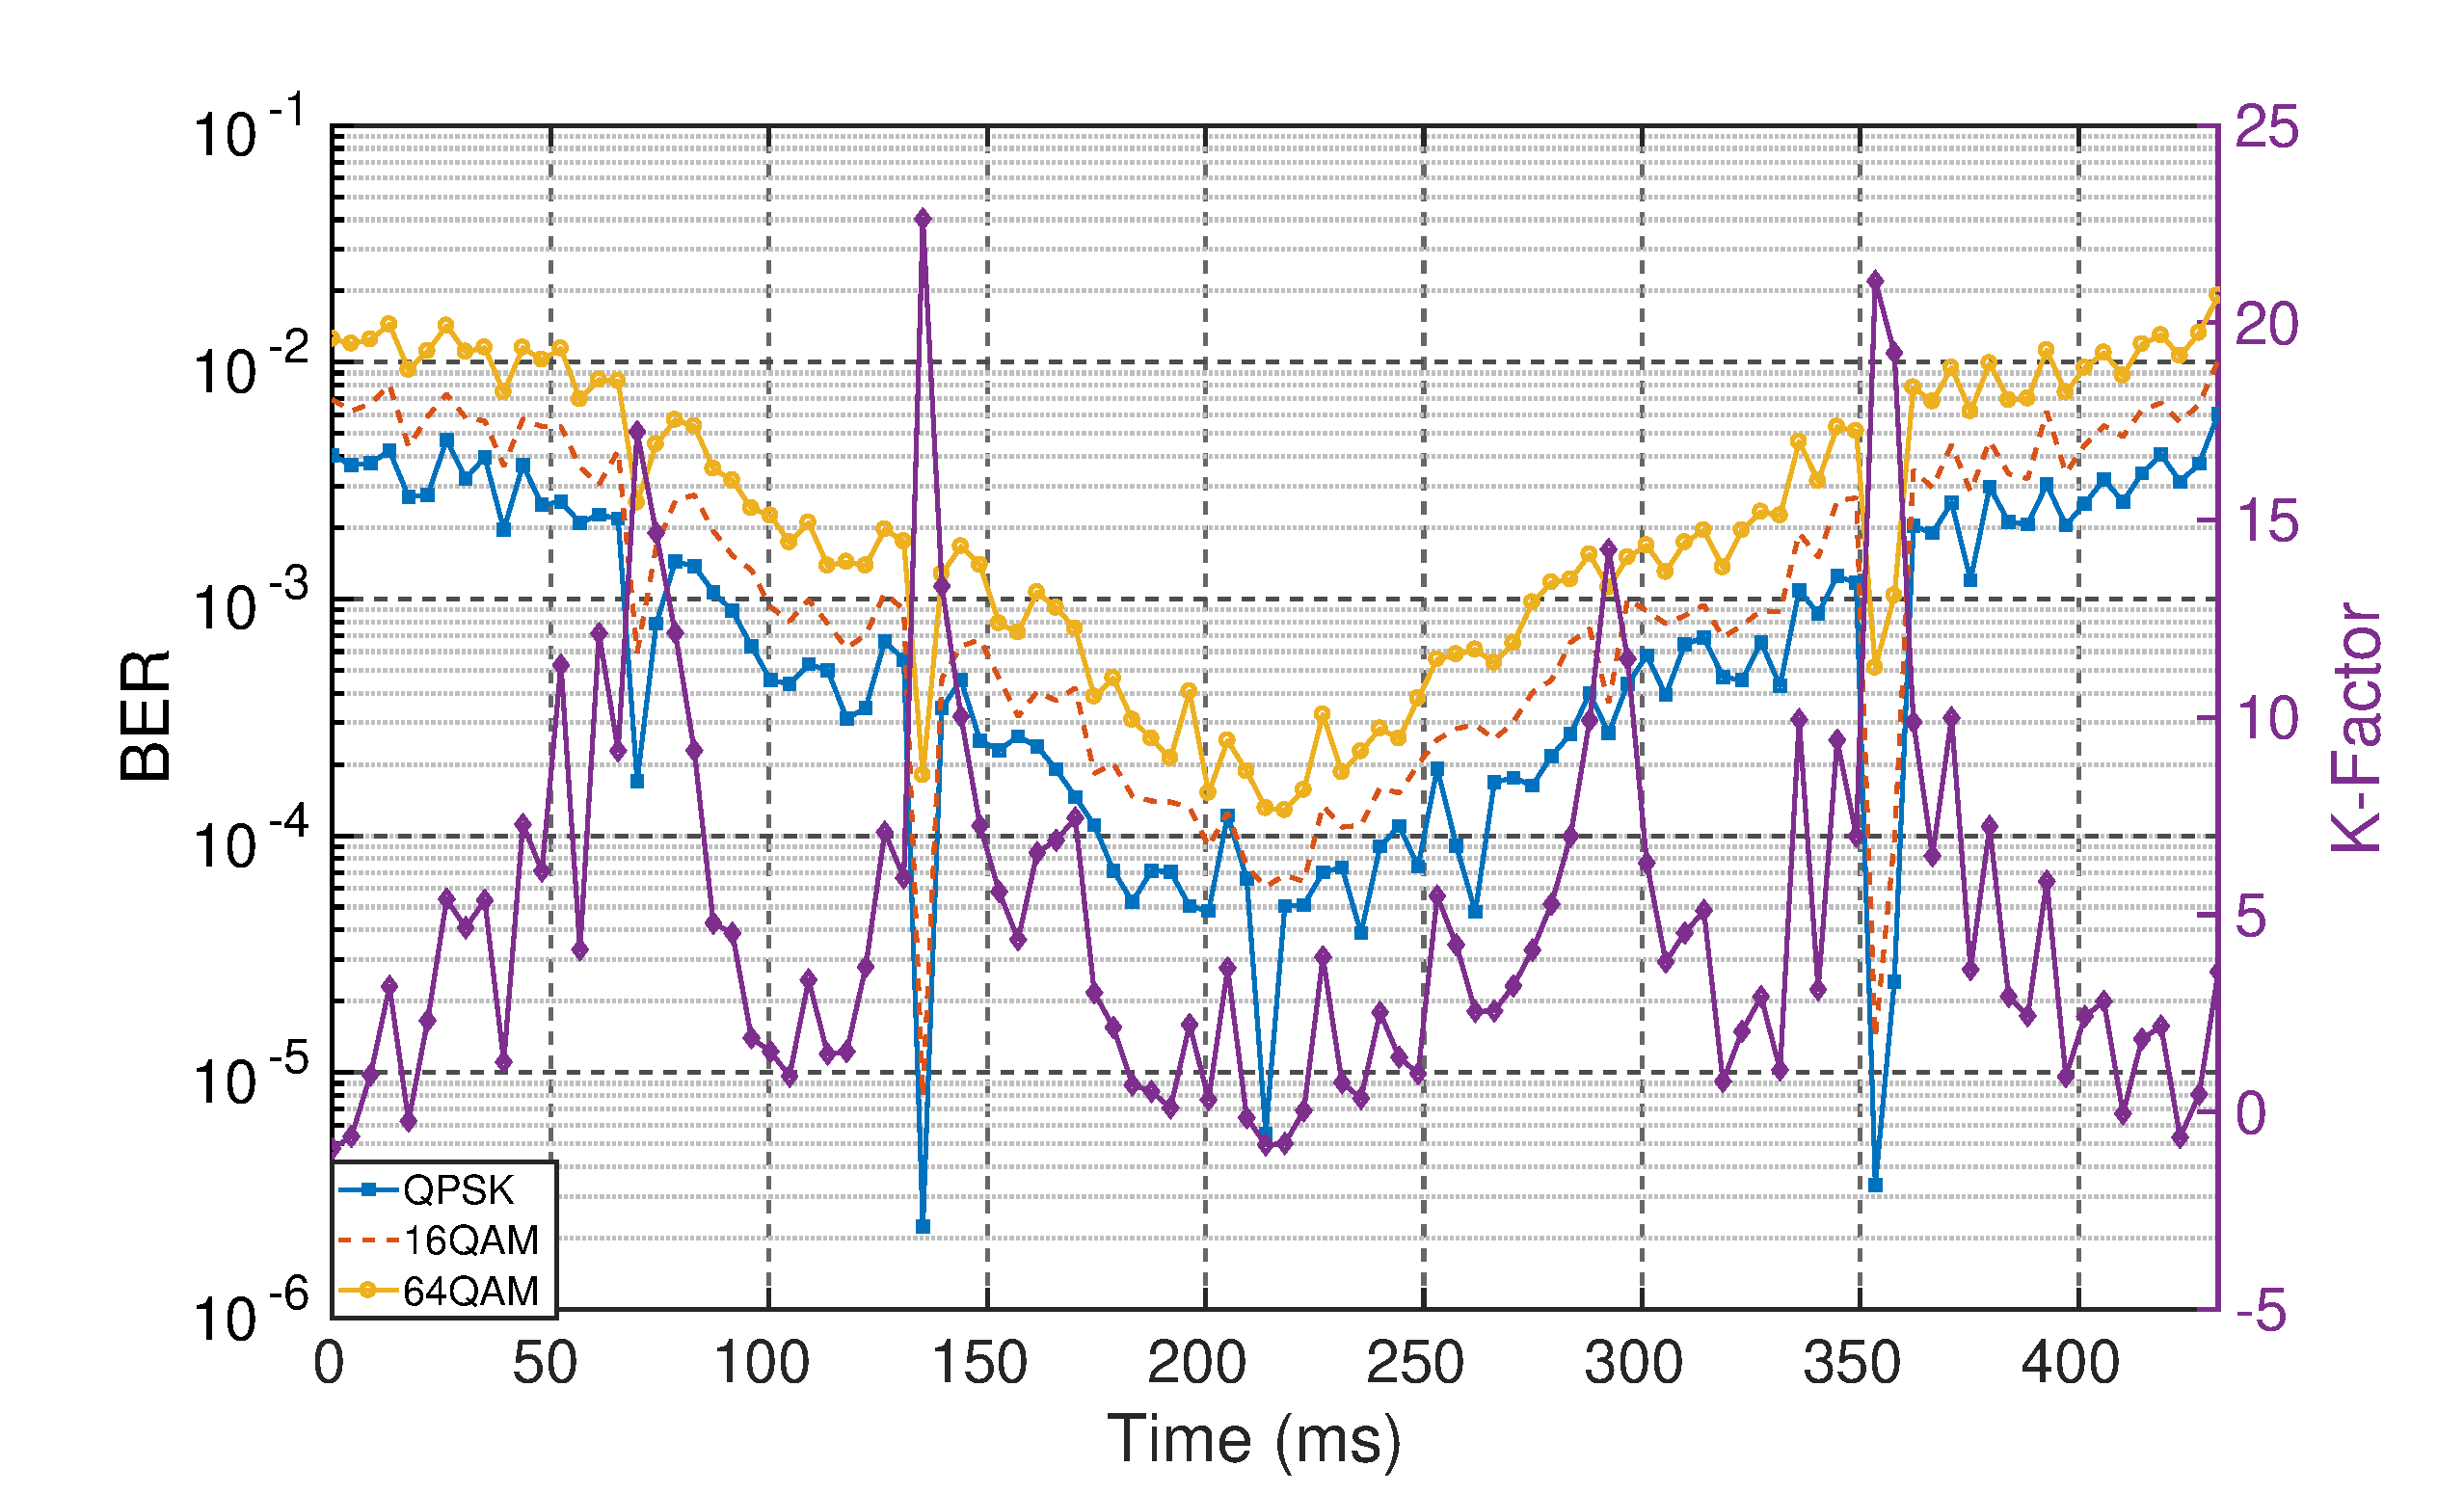
\includegraphics[width=\textwidth,keepaspectratio]{images/Gill/lte_figs/kfactorcontinuous.eps} 
\caption{BER variation with time for HST with different modulation schemes of LTE-R. As the train moves towards
the antenna the general trend of BER goes down with small-scale fluctuations due to varying K-factor.}
\end{figure}


\section{Channel Impairements Inside a Tunnel}
The tunnel environment is affected by multipath and diffraction effects due to multiple reflections from the tunnel walls, which leads to a substantial fading environment. By deploying LCX cables, we can eliminate the large penetration loss due to tunnel walls. However, small-scale fading can still cause a large amount of errors and decrease the QoS for the communication link. High velocity trains experience very high Doppler shifts and a fast fading channel. These problems can lead to significant BER degradation of the LTE system. The frequency shifts caused by the Doppler phenomenon can lead to shifts in the sub-carrier frequencies for OFDM, which leads to synchronization errors. The maximum Doppler shifts for a train traveling at 500 km/h is 2.314 kHz for a 5 GHz carrier frequency. This large Doppler shift can also lead to significant drops in the quality of wireless signals and increase the bit error rate. Thus,
to develop an efficient and reliable communication link inside tunnels, we need to properly model this channel impairment and build our proposed channel model by taking into account these tunnel phenomenons. These impairments are described in detail in the following subsections.

\subsection{Multipath Fading}
The following time-varying multipath channel impulse response considers the effects of Doppler shift and scattering~\cite{booklter13}:
\begin{equation}
\label{channel}
{h}(\tau,t)= \sum_{k=0}^{L}{h_k}(t)e^{-j2\pi f_c\tau_k(t)}\delta[\tau-\tau_k(t)],
\end{equation}
where $\tau$ is the path delay, $t$ is time in seconds, $\delta[\tau-\tau_k(t)]$ is the impulse response, $f_c$ is the carrier frequency, $h_k(t)$ is the envelope of the time-varying channel and consists of both large and small-scale fading components. Since the structure of LCX is almost the same as a leaky waveguide, the large scale fading of channel can be modeled linearly~\cite{arlter10}. There is also no signal shadowing and the line-of-sight (LOS) signal component is always present along the tunnel. This type of channel fading can be best described by a Ricean fading model. The probability density function $p(\alpha)$ of a Rician fading model is given by~\cite{inplter12}:
\begin{equation}
p(\alpha) = \dfrac{2\alpha(1+K)}{\Omega}I_0\Bigg(2\alpha\sqrt{\dfrac{K+K^2}{\Omega}}\Bigg)e^{\dfrac{-K-\alpha^2(1+K)}{\Omega}},
\end{equation}
where $K$ is the Rician factor and $\alpha$ is the complex amplitude of the channel response function that has a unity second moment, \textit{i.e.}, $\Omega \equiv E[\alpha^2] = 1$.

\subsection{Doppler Shift}
The 3GPP channel model~\cite{trlter14} is used for its Doppler shift profile in high speed railway environment. The measurements obtained for the Doppler frequency shift are implemented for two scenarios. The first scenario is for an open space while the second scenario is for high speed trains. Doppler shift is not taken into consideration. There exists a third scenario for tunnels using multiple antennas. Since the slots of LCX can be modeled as multiple antenna system, we use this Doppler shift profile for our proposed channel. The Doppler shift variation $f_s(t)$ is described by:

\begin{equation}
\label{eq1}
f_s(t) = f_d\cos\theta(t),
\end{equation}
where \textrm{$f_d$} is the maximum Doppler shift, $\theta$ is the elevation angle and $\cos \theta(t)$ is given by:
\begin{equation}
\cos\theta(t) = 
\left\{
	\begin{aligned}
	 & \dfrac{D_s/2-vt}{\sqrt{\mathrm{D_{min}}^2+\bigg((D_s/2)-vt\bigg)^2}},0\leq t\leq\dfrac{D_s}{v}\\
	 & \dfrac{-1.5D_s+vt}{\sqrt{\mathrm{D_{min}}^2+\bigg((-1.5D_s)-vt\bigg)^2}},\dfrac{D_s}{v}\leq t \leq \dfrac{2D_s}{v}\\
 	\end{aligned}
\right.
\end{equation}
where $D_s/2$ is the initial distance of the train from base-station, and $\mathrm{D_{min}}$ is base-station (BS)-Railway track distance, both in meters; $v$ is the velocity of the train in \textrm{m/s}, $t$ is time in seconds.

\begin{figure}[!ht]
\label{doppler}
\centering
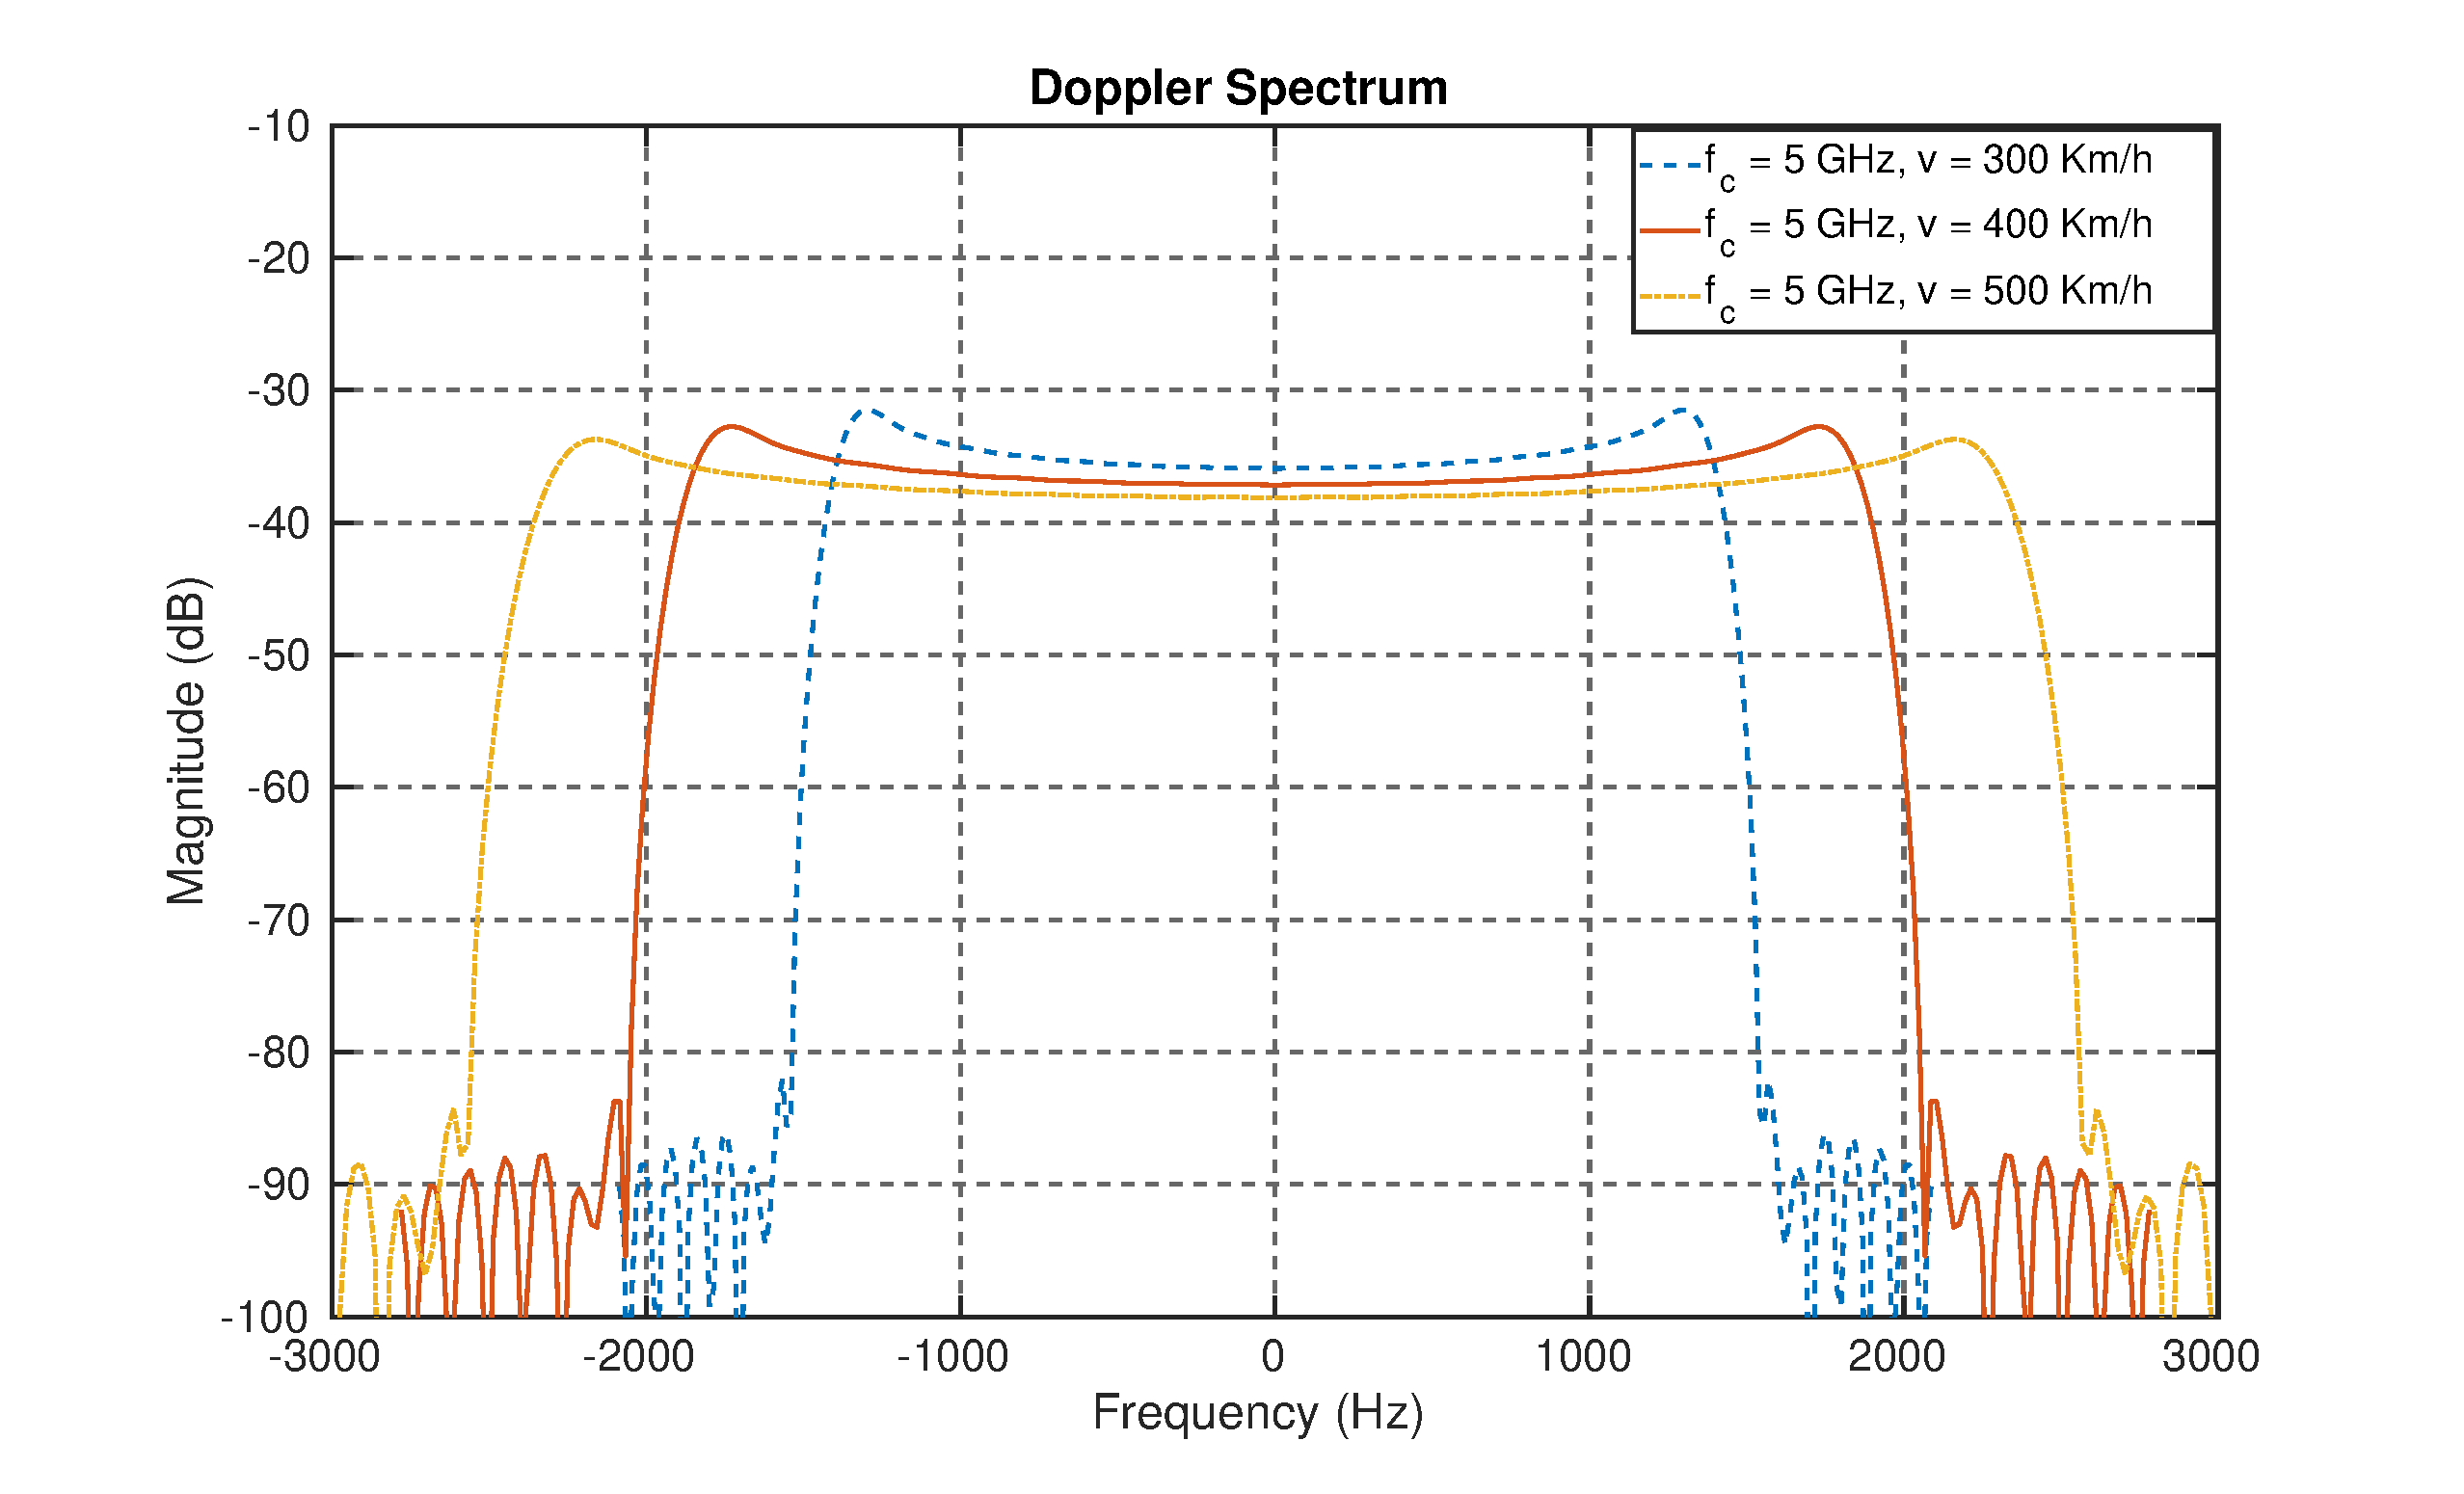
\includegraphics[width=\textwidth,keepaspectratio]{images/Gill/lte_figs/dopplerspectrum.eps} 
\caption{Doppler spectrum for LTE-R at different train velocities $v$ (km/h) = 300, 400 and 500 and $f_c$ = 5 GHz.}
\end{figure}

Figure~\ref{doppler} shows the Doppler spectrum for $f_c$ = 5 GHz and $v$ = 300 Km/h, 400 Km/h and 500 Km/h, and as we can see in the figure the maximum Doppler shift range is from -2.314 kHz to +2.314 kHz. These range of Doppler shift values can lead to very high bit-error rate and poor connectivity in communication system. In the following section we discuss our proposed channel model which consists of Doppler shift profile for high speed train and dynamic K-factor for tunnel environment.

\section{Proposed Channel Model}

The tunnel measurement campaign conducted in~\cite{inplter8} shows that the amplitude variation inside tunnel follows Rician distribution. In the thesis, we apply the approach used in~\cite{inlter15} for single elevation angle $\theta$ and expand it to a time-varying case. In this thesis, we model $\theta$ as a function of time and derive time-series $K$-factor for the tunnel environment. Figure~\ref{subblock} describes our proposed channel model which is implemented using dynamic K-factor and Doppler shift profile derived using Eq.(\ref{eq1}).  In the following section we discuss the classical two-ray propagation model and mathematical derivation of dynamic K-factor for our proposed channel model.

\begin{figure}[!ht]
\label{subblock}
\centering
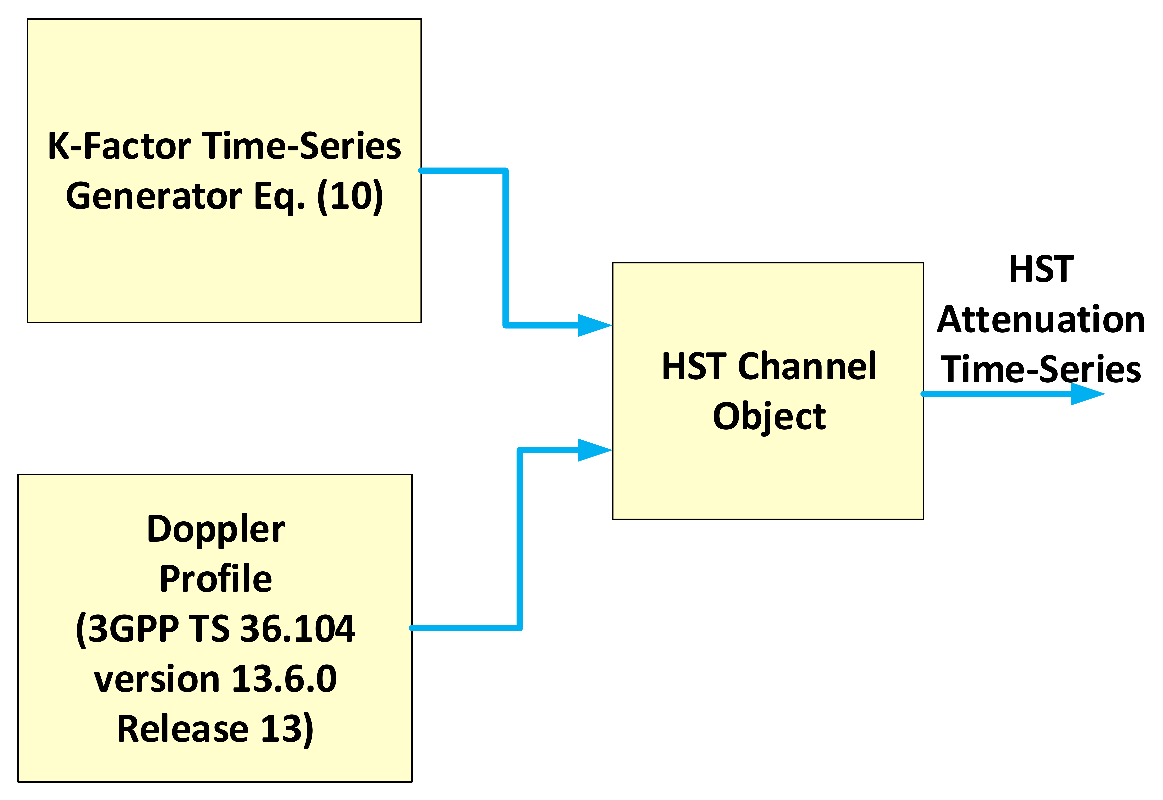
\includegraphics[width=\textwidth,height=6cm,keepaspectratio]{images/Gill/lte_figs/subblock.eps} 
\caption{HST channel model consisting of time-series K-factor and Doppler shift caused due to velocity of the train.}
\end{figure}

The reflection coefficient $\Gamma$~\cite{booklter16} as a function of time $t$ is given by:
\begin{equation}
\Gamma(t) = \dfrac{C\sin\theta(t)-\sqrt{(\varepsilon_r-j\chi(t))-(\cos\theta(t))^2}}{C\sin\theta(t)-\sqrt{(\varepsilon_r-j\chi(t))-(\cos\theta(t))^2}},
\end{equation}
where $C = 1$ is for horizontal polarization, and $C = \varepsilon_r-j\chi(t)$ for vertical polarization. Furthermore, $\chi(t)$ is given by:
\begin{equation}
\chi(t) = \dfrac{\sigma}{\omega(t)\varepsilon_0} = \dfrac{\sigma}{2\pi f_r(t) \varepsilon_0} = \dfrac{1.8\times 10^{10}\sigma}{f_r(t)}.
\end{equation}
with $\varepsilon_0 = 8.854\times 10^{-12}~\textrm{F/m}$, and $\sigma$ is conductivity of the tunnel. The frequency $f_r(t)$ is the resultant frequency caused by the Doppler shift and is given by:
\begin{equation}
f_r(t) = f_c(t)-f_s(t)
\end{equation}
where $f_c(t)$ is the sub-carrier frequency, and $f_s(t)$ is the Doppler shift given by Eq.~(\ref{eq1}).

The phase difference function of $t$, $\Delta\phi(t)$ between the two reflected paths is given by~\cite{booklter11}:
\begin{equation}
\begin{split}
\Delta\phi(t) =& \dfrac{2\pi}{\lambda(t)}\bigg(\sqrt{D_{\textrm{LOS}}^2+(h_t+h_r)^2}-\\
& \sqrt{D_{\textrm{LOS}}^2+(h_t-h_r)^2}\bigg),
\end{split}
\end{equation}
where $\lambda(t)$ is the resultant time-varying wavelength at the receiver, $D_{\textrm{LOS}}$ is the distance between the transmitter and receiver antennas which is changing dynamically with $t$, and both $h_t$ and $h_r$ are the heights of the transmitter and receiver antennas, respectively.
 
The resultant received power $p_r(t)$ is given by the sum of the LOS received power plus the received multipath power, resulting in:
\begin{equation}
\begin{split}
p_r(t) =& ~p_t(t)\bigg(\dfrac{\lambda}{4\pi d}\bigg)^2G_t G_r\bigg[1+\\
& |\Gamma(t)|^2+2|\Gamma(t)|\cos(\angle\Gamma(t)-\angle\Delta\phi(t))\bigg]
\end{split}
\end{equation}
which is a function of the transmitter power $p_t(t)$ and the reflection coefficient $\Gamma(t)$, where $G_t$ and $G_r$ are the transmitter and receiver antenna gains,  respectively.
The $K$-factor is defined as the ratio of the direct path power and the power in the scattered paths, and is given as:
\begin{equation}
\label{kfactor}
\mathrm{K}(t) = \dfrac{1}{|\Gamma(t)|^2+2|\Gamma(t)|\textrm{cos}(\angle \Gamma(t)-\Gamma(t)\Delta\Phi(t))}
\end{equation}

\section{Summary}
We analyzed the BER performance of a LTE-R system for high speed trains inside tunnel environments using our proposed channel model. For the implementation
of our channel, we first derived the time-series K-factor function using the classical two-ray propagation model. We then analyzed the LTE-R performance under our channel model for different modulation schemes for various K-factors. Finally, we compared all the modulation schemes under worst and best K-factor, and we observed that for low $E_b/N_0$
sub-carriers must be modulated with QPSK for maintaining reliable communication link.



%% LTE-R Implementation..
\chapter{Proposed Heterogeneous CSS Prototype}
\label{chapter5}

This chapter outlines the implementation of heterogeneous test-bed for cooperative spectrum sensing using USRP N210 and RTL-SDR software defined radios. We start with heterogeneous cooperative spectrum sensing, where we first describe the experimental setup, which is implemented using soft and hard fusion schemes. The sensor nodes, which consists of three RTL-SDRs and one USRP N210, are placed in a controlled indoor laboratory environment approximately 8-10 meters apart. The signal source is being simulated by another USRP N210, which is transmitting a DQPSK signal at 450 MHz. The post-processing is done on a Fusion Center (FC), which makes the decision based on global test statistic using both soft and hard decision schemes. Finally, we discuss the results where the performance of both the schemes are evaluated in a real fading scenario on a hardware test-bed. 

\section{Experimental Setup for Proposed Heterogeneous CSS Prototype}

The measurements are performed using software-defined radios (SDRs) and the post-processing is conducted on desktop computers. The desktop computer consists of i7 Intel processor with eight cores and 3.41 GHz clock cycle running Ubuntu 16.04. The sensor node network is implemented using RTL-SDR dongles and Ettus Research USRP N210 on GNU Radio Software platform. The measurements are analyzed in MATLAB and measurement plots are generated. Figure~\ref{expsetup} presents a photograph of the actual proposed prototype system, which consists of three RTL-SDRs and two USRP N210s. One USRP N210 (middle) acts as a primary user while the other SDRs operate as sensor nodes. All the SDRs were placed in a laboratory environment at least 5-6 meters away from the primary user.

\begin{sidewaysfigure}
\centering
	\includegraphics[width=\textwidth]{images/Gill/figs/setup.eps} 
\caption{Experimental Test-Bed For Cooperative Sensing in Heterogeneous Network. Sensors 1, 2 and 4 are RTL-SDR units, sensor 3 is USRP N210 and TX is another USRP N210 unit which is used as a signal source for this work.}
\label{expsetup}
\end{sidewaysfigure}

These sensor nodes collect the spectral data, normalize it, and then transmit it to the FC for the detection. For soft data fusion, the data is quantized in the local sensor nodes before it is transmitted to FC due to the limited bandwidth of the overhead channel. The delays caused by the different sensor nodes is ignored, as it would require extra computational complexity and it is out of the scope of this thesis. The USRP N210 transmits a DQPSK modulated signal with 4 samples per symbol with the alpha factor of the root raised cosine filter set to 0.35. The transmitter gain and amplitude are varied in order to get different SNR values for each node. The sensor nodes collect the data via 300,000 energy samples, and each measurement is conducted three times in order to eliminate any irregularities. The noise variance $\sigma_n^2$ for each SU is estimated by running each sensor node without any transmission at 450 MHz. The flow-graph is executed multiple times to get a better estimate of noise variance. Once the data is received from all the sensor nodes, the Probability of Detection ($P_d$) is calculated for different received SNR values for all the sensor nodes. To properly evaluate the performance of each of the cooperative spectrum sensing techniques, the average $P_d$ is calculated for each scheme. 

All four sensor nodes have different sampling rates to model potential differences existing within a heterogeneous environment. The USRP N210, which is also used as a $4^{th}$ sensor node, has a very low noise floor compared to the three other radios and hence can detect a signal with very low SNR. This is a challenging factor for data fusion when the nodes have different operating parameters and the FC has to make optimal decisions by combining this varying data. Due to their spatial diversity, the node closest to the transmitter will have different SNR compared to the other nodes. All these factors impact the data combining at the FC. The GNU Radio flow-graph for the sensor nodes is shown in the Figure~\ref{receiver}. The same flow-graph is used for all sensor nodes with different operating parameters. For the USRP N210 node, we replaced the RTL-SDR source with UHD:USRP Source gnuradio block. The central frequency is kept at 450 MHz and the operating parameters of each sensor node is provided in Table~\ref{tablehet}. The values of the transmitter amplitude and gain are varied to get the different sets of SNR values which are used for computing $P_d$ values for each node. The plots are generated in MATLAB by using the data files from the GNU Radio platform.

To evaluate the performance of the cooperative spectrum sensing, the USRP N210 is used as a transmitter, where its gain and amplitude are varied. Figure~\ref{transmitter} shows the flow-graph used for the transmitter. The flow-graph starts with the random source block, which generates the random data between zero and three, and passes it to the differential phase shift keying (DPSK) modulator block. The DPSK block modulates the signal with differential quadrature phase shift keying (DQPSK) scheme, applies root raise cosine filter with excess bandwidth value of 0.35, and passes it to a multiply const block. It is used to control the SNR value and finally the data is dumped into the USRP N210 sink, which transmits the data over the air where other sensor nodes can estimate the signal presence using soft and hard decision schemes.

\begin{figure}[ht!]
	\centering
	\includegraphics[width=\textwidth,keepaspectratio]{images/Gill/figs/transmitter.eps}
    \caption{GNU Radio Flowgraph For Transmitter Running on USRP N210.} 
\label{transmitter}      
\end{figure}

\begin{figure}[ht!]
	\centering
	\includegraphics[width=\textwidth,keepaspectratio]{images/Gill/figs/normalizedenergy.eps}
    \caption{GNURadio Flowgraph For USRP and RTL-SDR sensor nodes.} 
\label{receiver}      
\end{figure}

\begin{table}[!ht]
\caption{Operating Characteristics of Sensor Nodes}
\centering
\vspace{-5pt}
\begin{tabular}{c c c c c}
\toprule
Nodes      & $F_s$     & Gain  & FFT Size &  Bin Size \\ \hline
RTL-SDR-1  & 1.1 Msps  & 10 dB & 512      & 2.148 KHz \\ \hline
RTL-SDR-2  & 1.8 Msps  & 10 dB & 512      & 3.515 KHz\\ \hline
RTL-SDR-3  & 2.4 Msps  & 10 dB & 512      & 4.687 KHz\\ \hline
USRP N210  & 7.2 Msps  & 10 dB & 512     &  14.062 KHz\\ 
\bottomrule
\end{tabular}
\vspace{-5pt}
\label{tablehet}
\end{table}

The sensor nodes are placed inside the laboratory and are connected to distributed system. Figure~\ref{receiver} shows the flowgraph running on the receiver, for flow-graph running on USRP we use UHD:USRP source instead of RTL-SDR source. The frequency around 450 MHz is sweeped in regular intervals and the continuous data stream is passed to FFT block, which does the forward FFT operation with a Blackmann Harris window. The data is first converted into parallel stream of the FFT size using stream to vector GNU Radio block. The complex-to-magnitude block converts the complex values into float and take their magnitude. The bin selector block is used to select the bin where the narrowband signal is being transmitted. We then take the moving average of the values, normalize them and then store it to the file sink. The normalized energy values are collected for each sensor at different SNR values and then post processing is performed in MATLAB. The operating parameters of each sensor node is provided in the Table~\ref{tablehet}.

\section{Hard-Data Fusion Scheme}
\label{hardfusion}
Cooperative spectrum sensing using hard-data fusion is a proven method for improving the detection performance. In this scheme, all sensor nodes sense the signal source individually and send their sensing decision in the form of 1-bit binary data. For hard data fusion, the noise $w_q$ can be neglected since the sensor nodes can just transmit their decision statistic in an efficient way, where the floating values are not required. For example, the SUs can just transmit ''1'' and ''0'' depending on whether the primary user is present or absent. Furthermore, in the Fusion Center the decision can be made by using the OR, AND, or majority rule algorithms. For the AND decision rule, the FC performs the logical AND operation for all the local decisions and conducts the detection. Similarly, for the OR rule, the logical OR operation is used to decide whether the signal is present or not. Finally, the majority rule conducts majority vote and decides based on it~\cite{ghasemi2005collaborative,duan2010performance}. The $P_d$ for AND, OR and Majority Rule for $R=4$ sensor nodes is given by~\cite{inphtn15}:
\begin{equation}
P_{d,AND} = (P_d)^4\nonumber\\
\vspace{-15pt}
\end{equation}
\begin{equation}
\label{hard}
~~~~~~~P_{d,OR} = 1-(1-P_d)^4
\vspace{-15pt}
\end{equation}
\begin{equation}
P_{d,MJR} = 6P_{davg}^2(1-P_{davg})^2+4P_{davg}^3(1-P_{davg})+P_{davg}^4\nonumber
\end{equation}
where $P_{davg}$ is the average probability of detection of the sensor units. Similarly, we can calculate the $P_{fa}$ for all three schemes by replacing $P_{davg}$ by $P_{faavg}$ in Eq~(\ref{hard}).

\begin{figure}[ht!]
	\centering
	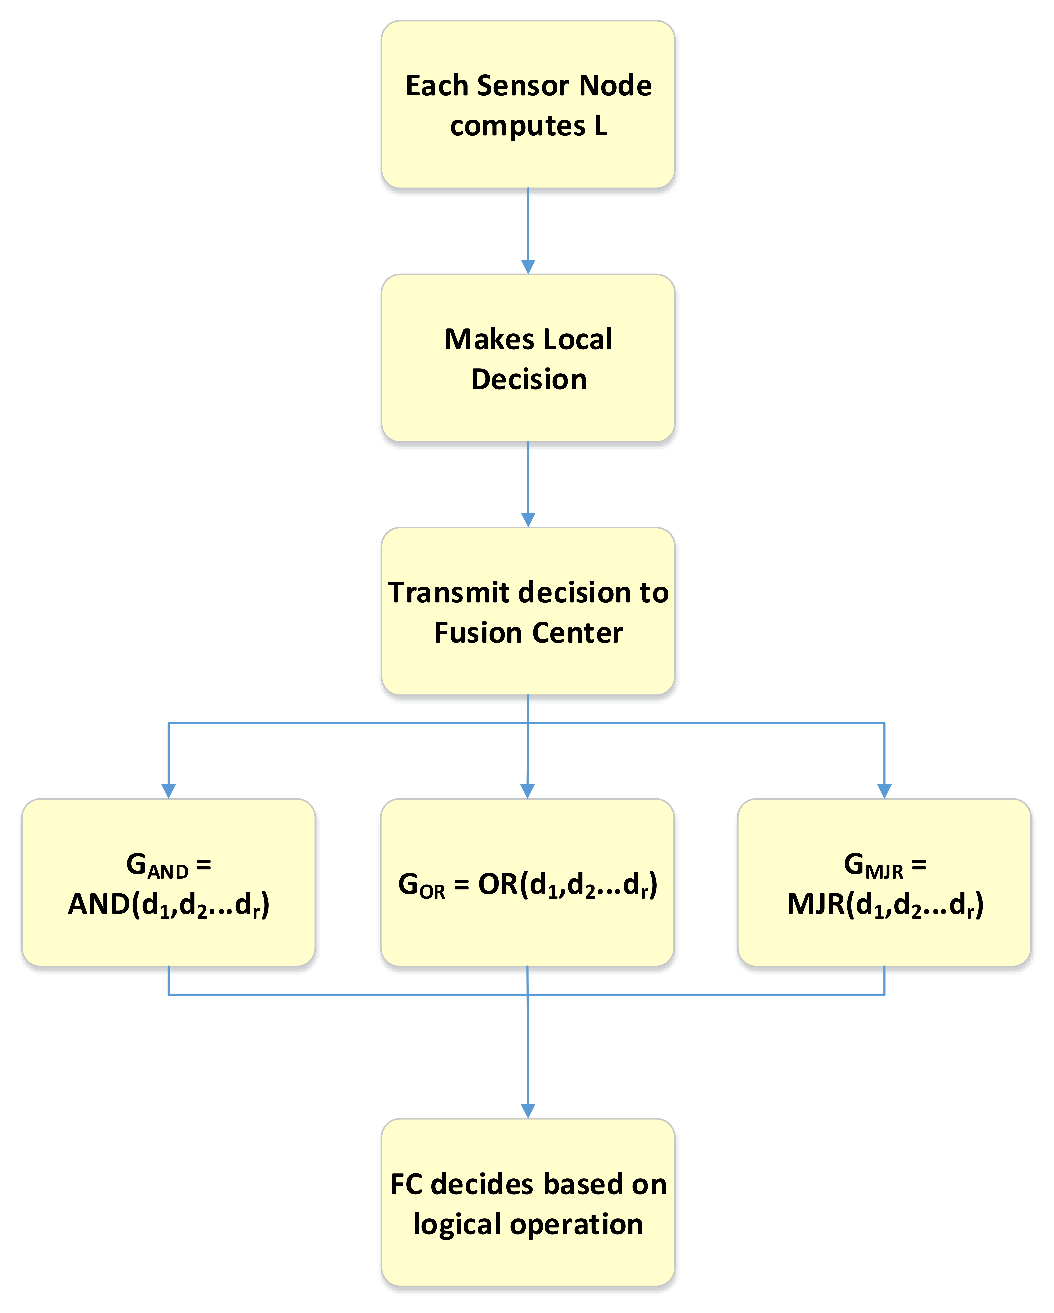
\includegraphics[width=\textwidth,height=10cm,keepaspectratio]{images/Gill/figs/hardfusion.eps}
\caption{Flowchart showing AND, OR and Majority Rule Fusion schemes.} 
\label{hard}      
\end{figure}

\section{Soft-Data Fusion Scheme}

In soft-data fusion based cooperative spectrum sensing, information from different CR users is combined to make a decision on the presence or absence of the primary user. In Section~\ref{hardfusion}, we discussed the conventional hard combination, where each CR user feedbacks one-bit message regarding whether observed energy is above a certain threshold. In this section, we discuss soft combination of the local test statistic of each sensor nodes and how it is combined to make the decision in the FC. Since in the soft combination accurate energy values from different CR users are utilized to make a decision, this scheme is more accurate and complex to implement. In this thesis, we discuss two popular soft decision fusion schemes: \textit{Maximum Normalized Energy} (MNE) scheme and \textit{Equal Gain Combining} (EGC) scheme.

For MNE, the local test statistic in each sensor node is computed and then transmitted to FC after quantization. In this thesis, we are using four sensor nodes equipped with different sensing abilities such as the sampling rates and noise floor. Therefore, the global test statistic $G$ can be modeled by:
\begin{equation}
\label{eq:8}
G_{MNE} = \max\{\beta_r\}.
\end{equation}
The $P_{fa}$ and $P_d$ values for the MNE-CS is given by~\cite{inhtn12}:
\begin{equation}
\label{eq:9}
P_{fa} = 1-\prod_{r=1}^R\Bigg(1-Q\Bigg(\dfrac{\tau-1}{\sqrt{\dfrac{1}{M_r}+\sigma_{q,r}}}\Bigg)\Bigg),
\end{equation}
\begin{equation}
\label{eq:10}
~~~~~~P_d = 1-\prod_{r=1}^R\Bigg(1-Q\Bigg(\dfrac{\tau-1-\gamma_r}{\sqrt{\dfrac{1+2\gamma_r}{M_r}+\sigma_{q,r}}}\Bigg)\Bigg),
\end{equation}
where $\tau$ is the global threshold for MNE, $M_r$ is the number of samples for $r^{th}$ sensor node, and $\sigma_{q,r}$ is the noise variance for the received local test statistic. The algorithm for MNE-CS is illustrated by the flowchart in Figure~\ref{mnescheme}.

\begin{figure}[ht!]
	\centering
	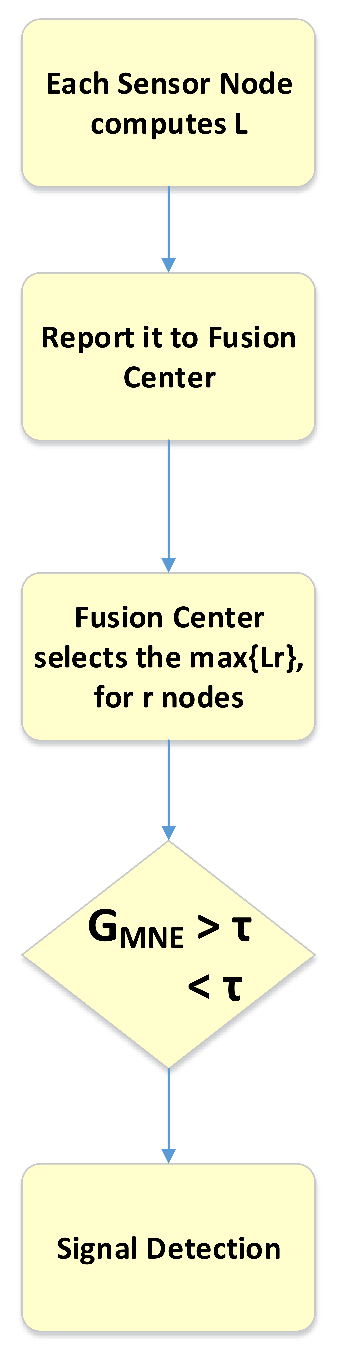
\includegraphics[width=\textwidth,height=10cm,keepaspectratio]{images/Gill/figs/mnescheme.eps}
\caption{Flowchart describing Maximum Normalized Energy Scheme.} 
\label{mnescheme}      
\end{figure}

For EGC, the global decision statistic is the mean of the $\beta$ values for all the sensor nodes. It has been shown in \cite{inhtn12} that the EGC scheme performs better than the MNE scheme in a noisy channel. The EGC scheme can be modeled by:
\begin{equation}
	\label{eq:11}
	 G_{EGC} = \dfrac{1}{M}\sum_{r=1}^{M}{\beta_r},
\end{equation}
where $G_{EGC}$ is global test statistic of EGC scheme. The $P_{fa}$ and $P_d$ values for the EGC-CS scheme are given by:
\begin{equation}
\label{eq:12}
P_{fa} = Q\Bigg(\dfrac{\tau-1}{\sqrt{\dfrac{1}{R^2}\sum_{r=1}^{R}\bigg(\dfrac{1}{M_r}+\sigma_{q,r}^2\bigg)}}\Bigg),
\end{equation}

\begin{equation}
\label{eq:13}
~~~~~~P_d = Q\Bigg(\dfrac{\tau-\dfrac{1}{R}\sum_{r=1}^R(1+\gamma_r)}{\sqrt{\dfrac{1}{R^2}\sum_{r=1}^{R}\bigg(\dfrac{1+2\gamma_r}{M_r}+\sigma_{q,r}^2\bigg)}}\Bigg).
\end{equation}
The algorithm for EGC-CS is also illustrated by the flowchart in Figure~\ref{egcscheme}.

\begin{figure}[ht!]
	\centering
	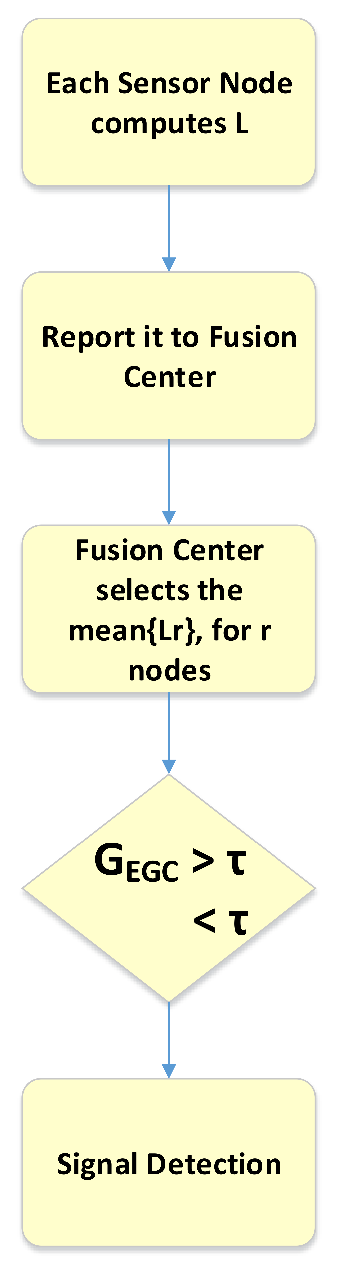
\includegraphics[width=\textwidth,height=10cm,keepaspectratio]{images/Gill/figs/egcscheme.eps}
\caption{Flowchart describing Equal Gain Combining Scheme.} 
\label{egcscheme}      
\end{figure}

\section{Experimental Results}
In this thesis, we implemented the heterogeneous cooperative spectrum sensing (CSS) using both hard and soft data fusion schemes. We start by collecting the data across 450 MHz band for all sensor nodes in a distributed manner. The spectrum sensing data is normalized for both soft and hard data fusion schemes using the same operational parameters to compare their performance accurately. The measurements are performed using software-defined radios (SDRs) and the post processing is conducted on desktop computers. The desktop computer consists of an i7 Intel processor with eight cores and 3.41 GHz clock cycle running Ubuntu 16.04. The sensor node network is implemented using RTL-SDR dongles and Ettus Research USRP N210 on GNU Radio Software platform.
These sensor nodes collect the spectral data, normalize it and then transmit it to the FC for the detection. For soft data fusion, the data is quantized in the local sensor nodes before it is transmitted to FC due to the limited bandwidth of the overhead channel. 

Figure~\ref{hardres} shows the $P_{davg}$ versus $SNR_{avg}$ for all four sensor nodes when hard decision combining is performed. It can be seen that OR performs the best, while AND performs the worst in a fading channel. The SNR average was computed by taking the mean of all the SNRs for the sensor nodes. The SNR was varied for each sensor node by varying the transmitter amplitude and gain in the GNU Radio flow-graph.

\begin{figure}[ht!]
	\centering
	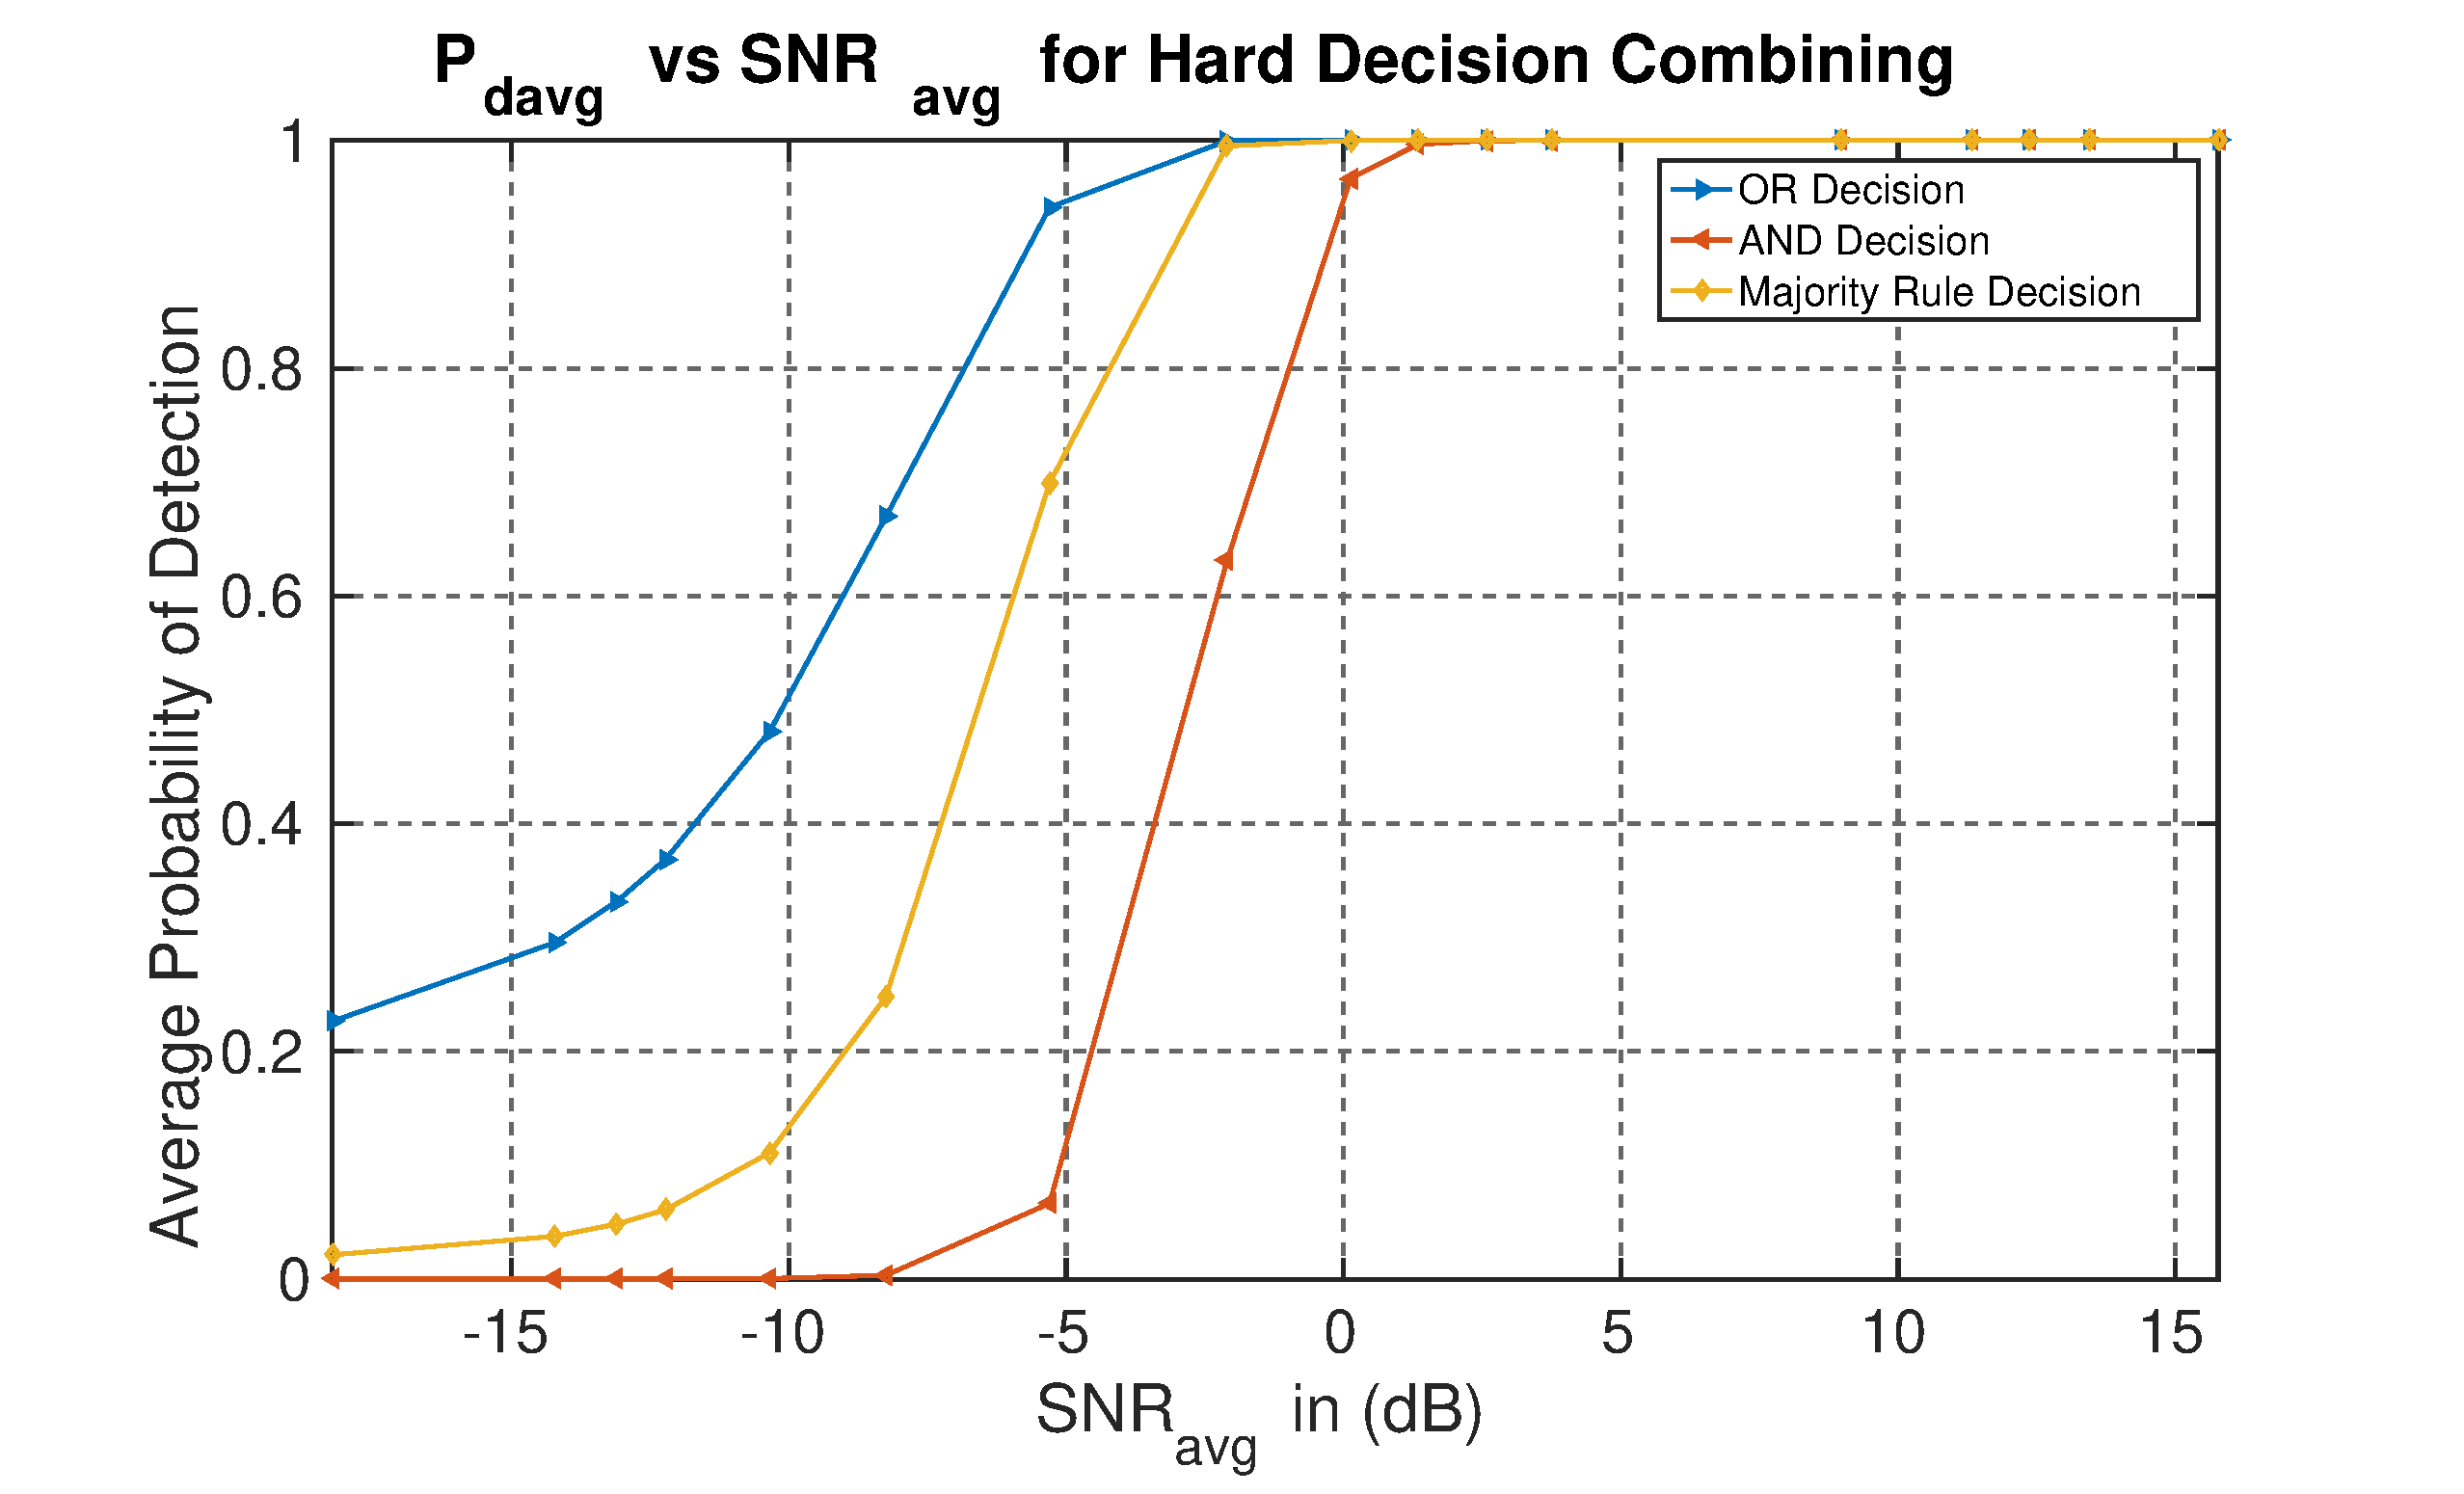
\includegraphics[width=\textwidth,keepaspectratio]{images/Gill/figs/hardecisionpd.eps}
    \caption{Probability of Detection versus $SNR_avg$ For Hard Decision Combining.} 
\label{hardres}      
\end{figure}

In Figure~\ref{hardroc}, the ROC characteristics for the hard decision combining at two different $SNR_{avg}$ for all three hard data fusion schemes are provided. It is pretty evident from the plot that the OR scheme performs better than both the AND and majority rule schemes. The AND scheme performs the worst because it depends on all sensor nodes to have same decision, which is very difficult in a real fading environment. For lower SNR values, OR outperform the majority rule by a large margin but as we go to higher SNR values their performance converges.

\begin{figure}[ht!]
	\centering
	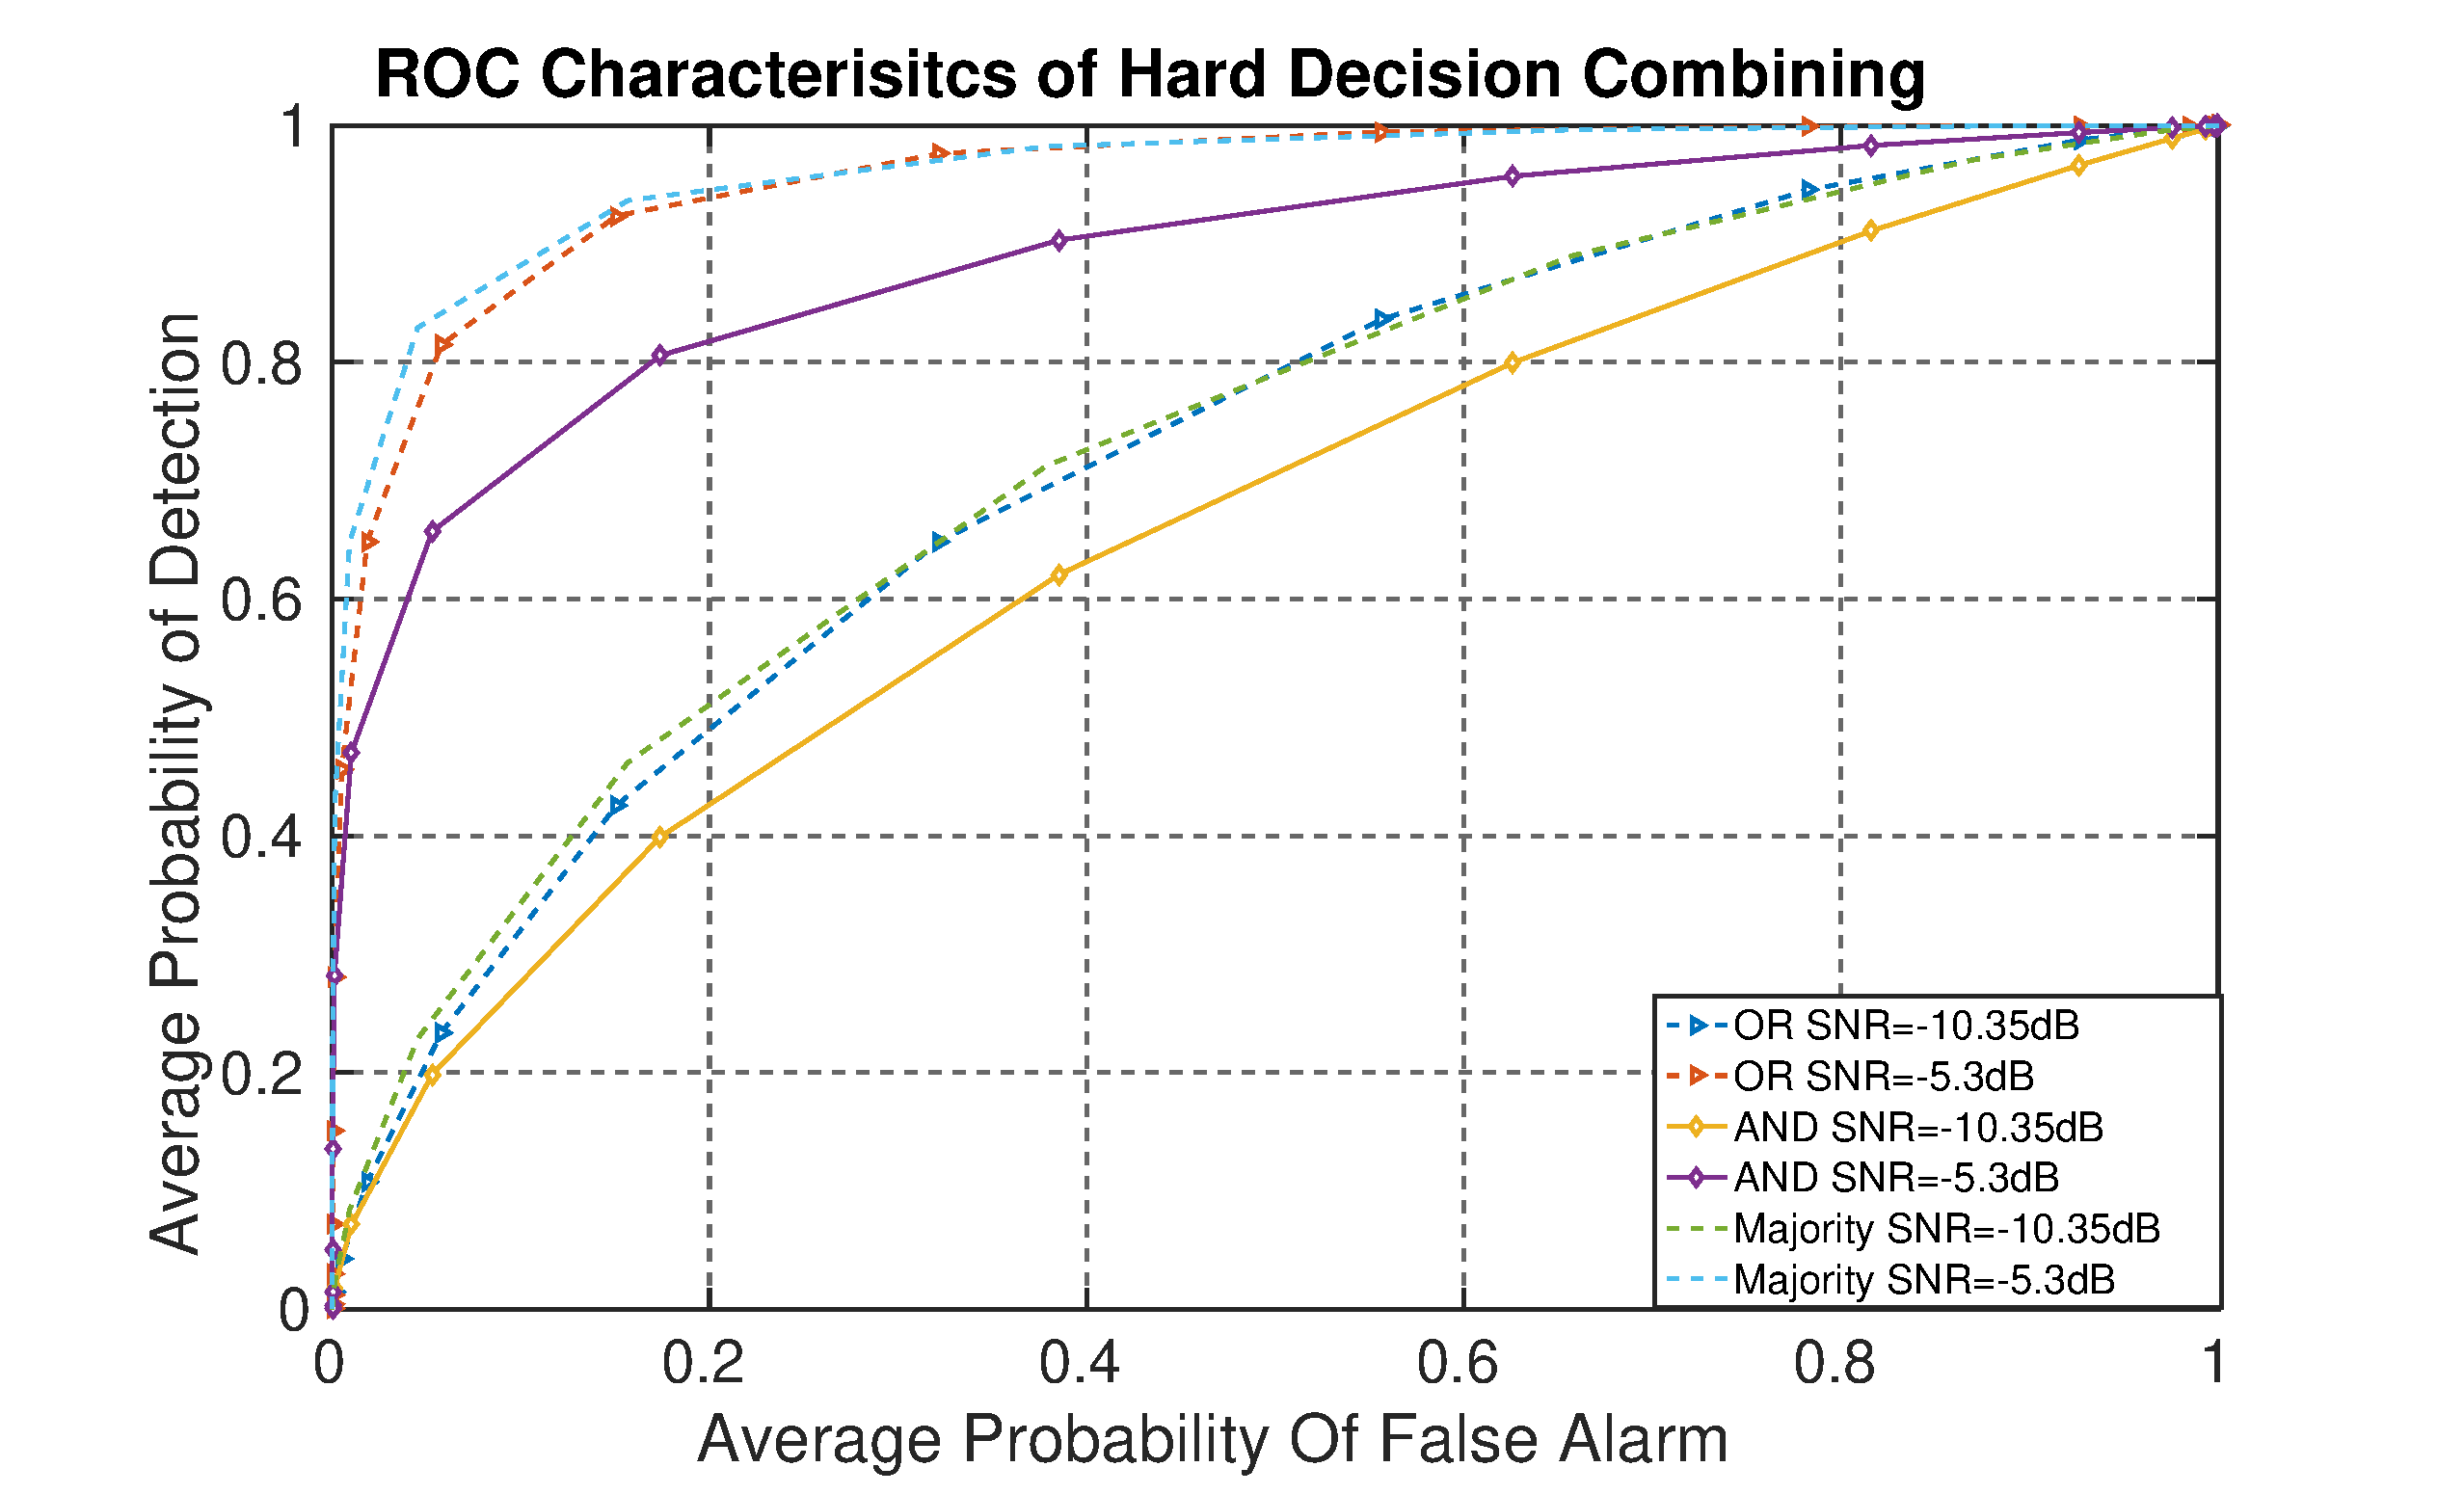
\includegraphics[width=\textwidth,keepaspectratio]{images/Gill/figs/hardecisioroc.eps}
    \caption{ROC Characteristics for Hard Decision Combining with Different SNRs.} 
\label{hardroc}      
\end{figure}

Figure~\ref{softpd} shows the $P_{davg}$ versus $SNR_{avg}$ for both soft and hard data fusion schemes. MNE and OR schemes overlap on the plot because in MNE scheme we take the maximum normalized energy and compare it the global test statistic, whereas for the OR scheme we estimate the signal source by either of sensor node decision. This makes both the scheme almost same and this is visible in the results. The EGC scheme performs the best since it takes into consideration all the sensor nodes and its global test statistic gives equal weight to all sensor nodes. The AND scheme performs the worst as expected. It is very important to understand that at higher SNR values, $SNR_{avg} > 2$ dB, we see all schemes converging to the same decisions. This tells us that in noiseless environment, we can choose hard fusion schemes because of their implementation complexity and we can select soft fusion in severe fading environment as they tend to be more accurate in these scenarios.
\begin{figure}[ht!]
	\centering
	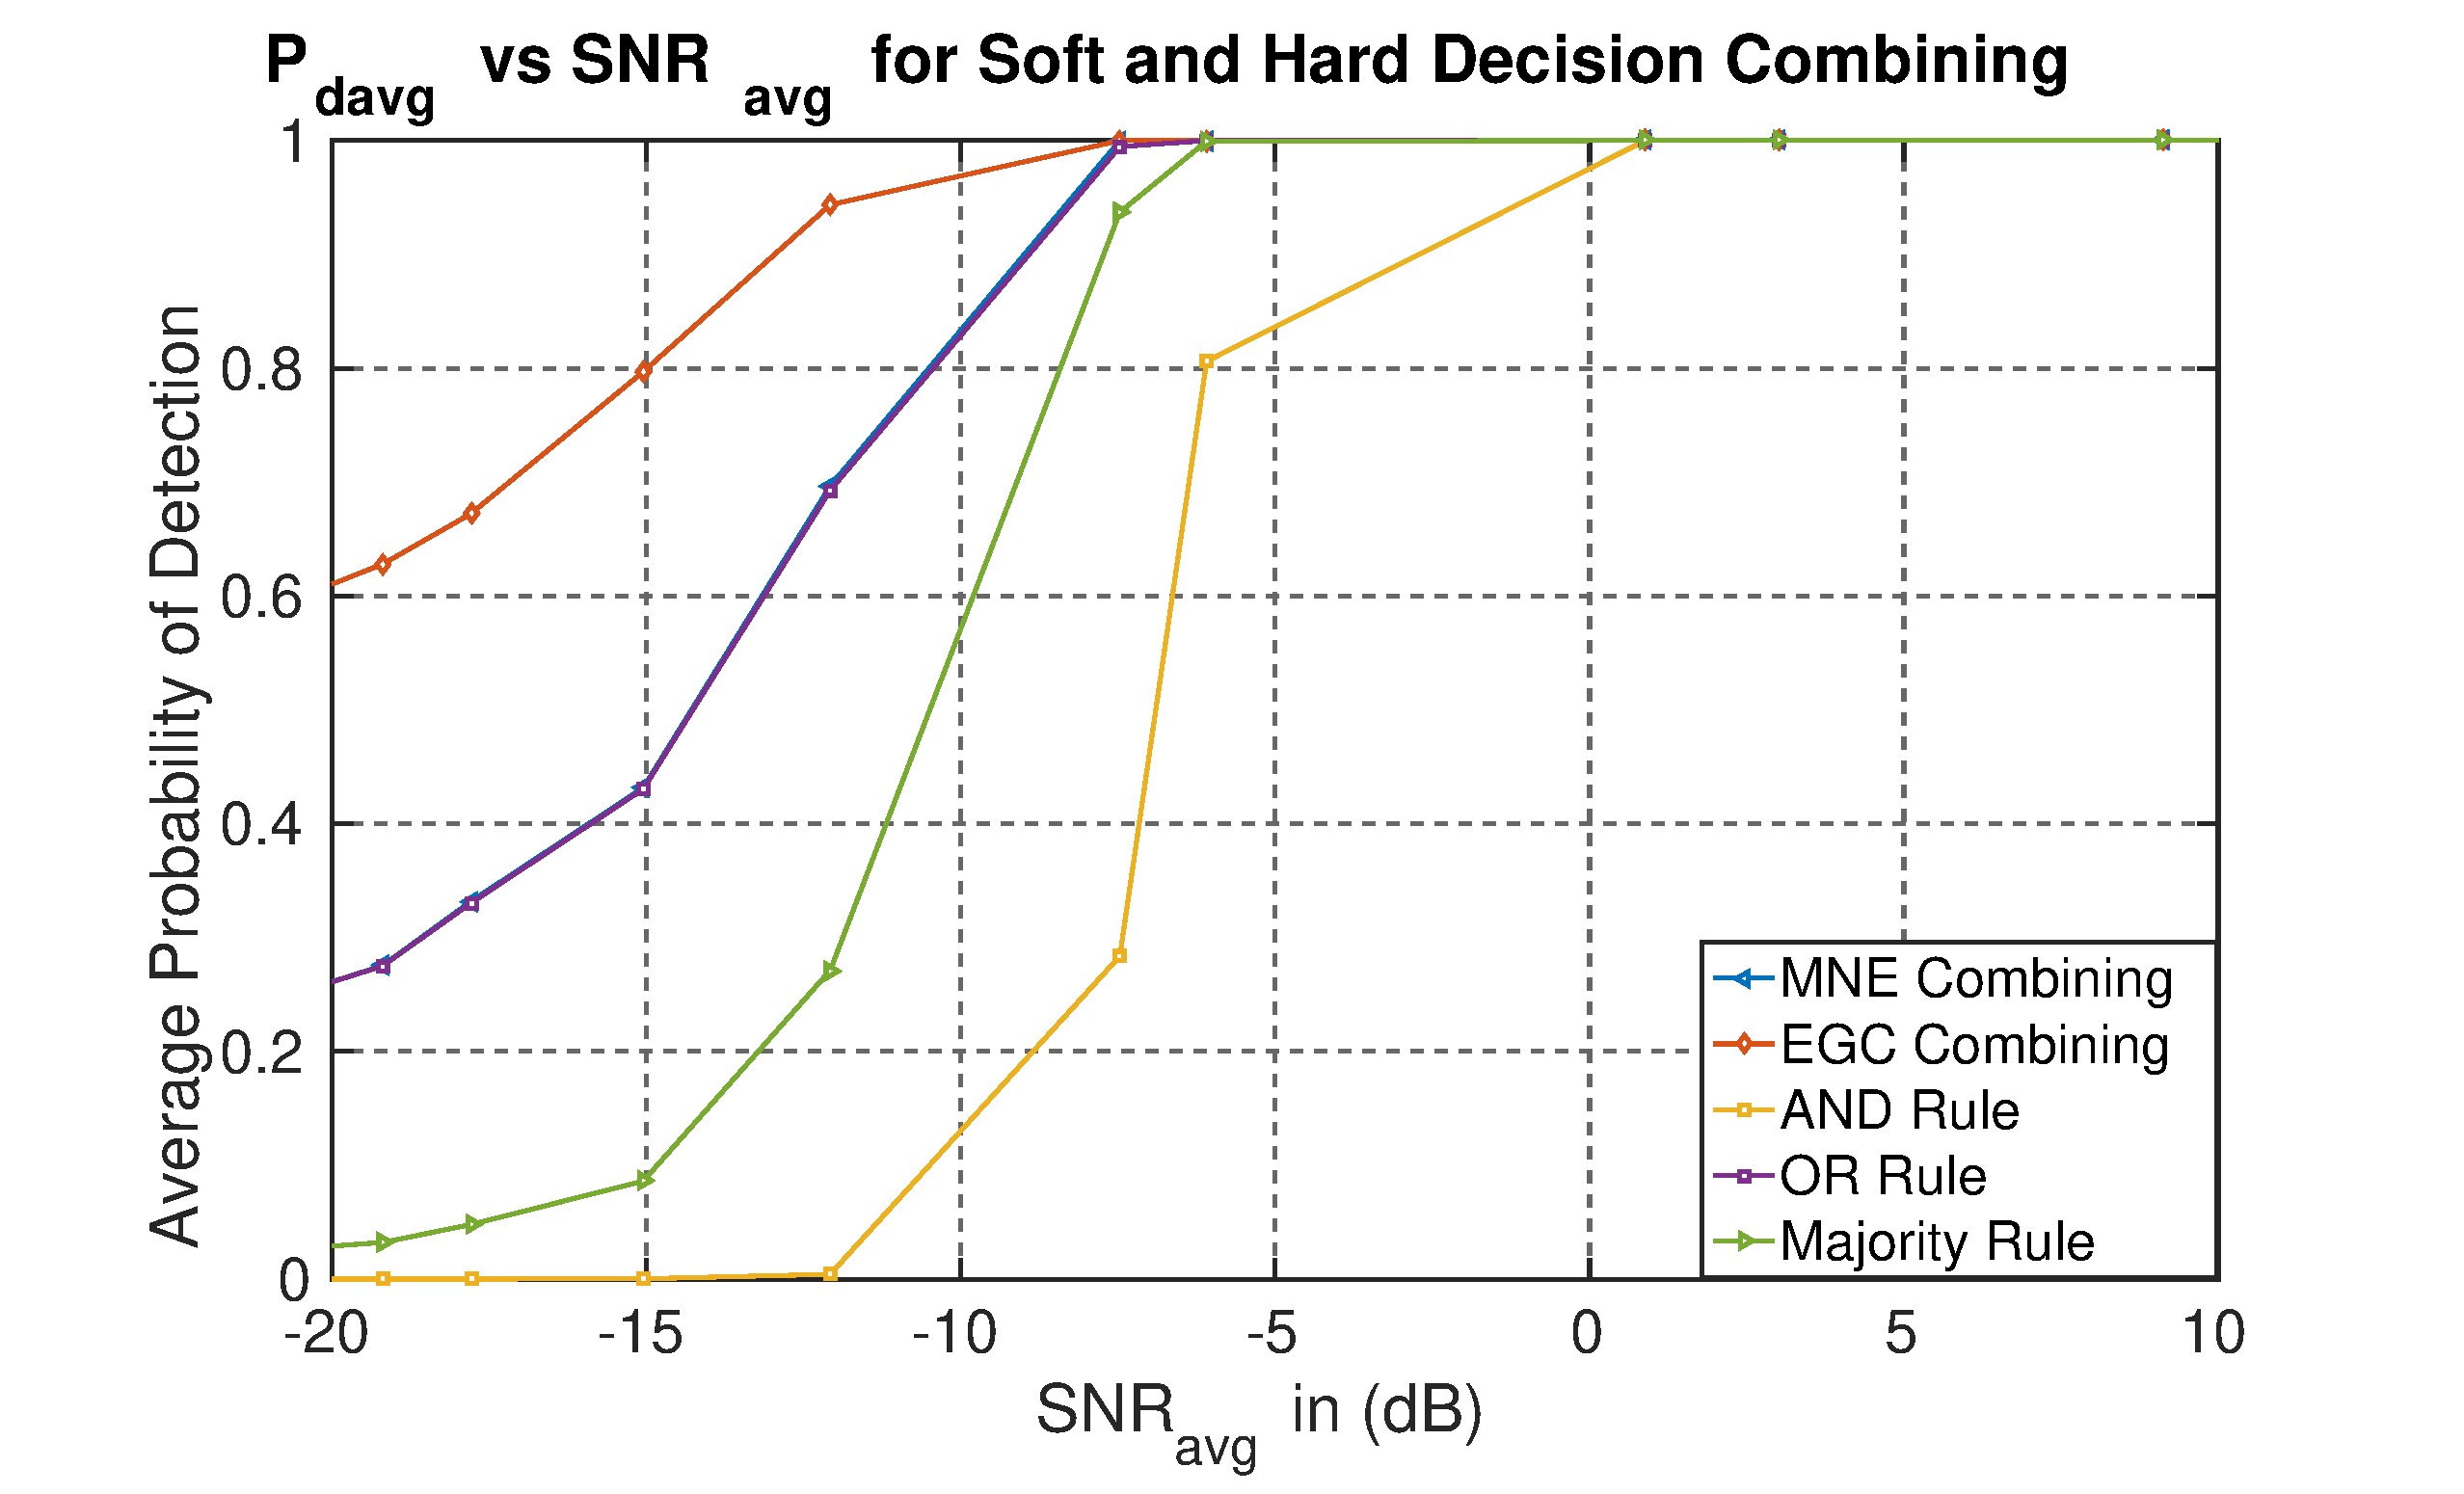
\includegraphics[width=\textwidth,keepaspectratio]{images/Gill/figs/softnhardecisionpd.eps}
    \caption{Probability of Detection versus $SNR_avg$ For Soft and Hard Decision Combining.} 
\label{softpd}      
\end{figure}

\section{Summary}
In this chapter, we described the test-bed setup using USRP N210 and RTL-SDR with different operating characteristics. The proposed heterogeneous CSS performance for both soft and hard data fusion approaches was derived at different SNR values. For soft-data fusion, scheme we use maximum normalized energy (MNE) and equal gain combining (EGC) scheme, and for hard data fusion scheme we used AND, OR and Majority Rule approaches. The results show that soft-data fusion scheme performs better than hard data fusion schemes for low SNR values, but as we increase SNR both schemes converges to same values. We learned that for severe environment, we can use soft-fusion and for noise-free environment hard decision schemes can be used due to their low implementation complexity.


%% Conclusion..
\chapter{Conclusions}
\label{conclusion}
This chapter summarizes the work as part of this project and then suggests related research that can be performed in the future. The research achievements includes implementation of test-bed for cooperative spectrum sensing in heterogeneous network, the performance measure of both soft and hard data fusion schemes in a real fading scenario. The simulation test-bed is implemented in MATLAB to test the performance of LTE-R in our proposed channel. The proposed channel is built on two-ray propagation model with time-series K-factor which we have derived mathematically and also uses Doppler shift profile for high speed trains. The future work section describes how we can take the mobility effect into the cooperative spectrum sensing and then test the performance of soft and hard fusion schemes in a mobile scenario. For LTE-R for future work we will use LTE antenna toolbox provided by MATLAB to implement the simulation test-bed which is more realistic and close to the actual system.

\section{Research Outcomes}
\begin{itemize}
\item We analyzed the BER performance of a LTE-R system for high speed trains inside tunnel environments using our proposed channel model. For the implementation of our channel, we first derived the time-series K-factor function using the classical two-ray propagation model.

\item We then analyzed the LTE-R performance under our channel model for different modulation schemes for various K-factors. Finally, we compared all the modulation schemes under worst
and best K-factor, and we observed that for low $E_b/N_0$ sub-carriers must be modulated with QPSK for maintaining reliable communication link.

\item The last plot shows the BER curve for discrete time-step when the train is moving with a velocity of 500 Km/h and carrier frequency for all modulation scheme is set to 3 GHz.The plot is also overlayed with continuous K-factor variation with the propagation of the train. It can be observed from the plot that as the K-factor goes high the BER drops, which represents the train moving towards the LCX slot. 

\item As the train move away from the slot the BER starts increasing. For reliable and efficient communication links the sub-carriers have to be modulated with QPSK for low K-factor values, or more LTE repeaters are required inside the tunnel to get good connectivity. However, the most important factor that has to be taken into consideration is the real-time channel equalization to reduce the BER rate.

\end{itemize}

\section{Future Work}
\begin{itemize}
\item In this paper, we conducted an experimental study for cooperative spectrum sensing using normalized energy detection for
both soft and hard decision combining techniques. It was found that the soft fusion schemes works better than hard decision for real fading environment with low SNR values. 

\item For higher values, all schemes converged to the same decision which led us to conclude that hard fusion schemes pays better when the environment is less noisy due to their low complexity as compared to soft fusion. For future work, it is worth exploring an increase in the number of nodes and adding mobility for the testing the performance of heterogeneous networks in a time-variant channel.

\end{itemize}

%%%%%%%%%%%%%%%%%%%%%%%%%%%%%%%% THE FINISH %%%%%%%%%%%%%%%%%%%%%%%%%%%%%%%
%SEE HERE for BIBTEX styles: http://www.cs.stir.ac.uk/~kjt/software/latex/showbst.html
\bibliographystyle{IEEEtran}

\bibliography{mybib}

\appendix
%\addtocontents{toc}{\protect\contentsline{chapter}{\protect\numberline{}Appendix:}{}{}}
\chapter{Heterogeneous Cooperative Spectrum Sensing Code}
\section{harddecisionpdroc.m}
\begin{lstlisting}[breaklines]
% Hard-Decision Combining Results For Sensor Nodes
clc;
close all;
clear all;
%% Parameter Initialization
N = 32;
k=4;%sensor nodes..
variance = 24.32e-9;
pfa = 0.05;
threshold = (qfuncinv(pfa)+sqrt(N)).*sqrt(N)*2*variance;
snrthreotical = -18:0.5:20;
snrlinear = 10.^(snrthreotical/10);
%% SNR values from USRP and RTL-SDR
snrpracticalavg = [-18.23,-14.22,-13.1,-12.22,-10.35,-8.25,-5.3,-2.1,0.13,...
    1.34,2.58,3.76,8.98,11.33,12.35,13.45,15.77];
snrlinearprac = 10.^(snrpracticalavg/10);
%% Computing Detection Probability and ROC Characteristics
pdprac = qfunc((threshold-2*N*variance.*(1+snrlinearprac))./...
    (sqrt(N.*(1+2*snrlinearprac))*(2*variance)));
pdpracor = 1-(1-pdprac).^4;
pdpracand = pdprac.^4;
tmp1 =  (1-pdprac).^2;
tmp2 = (1-pdprac);
pdpracmjr = (6*pdprac.^2).*tmp1+(4*pdprac.^3).*tmp2+pdprac.^4;

pfapracor = 1-(1-pfa).^4;
pfapracand = pfa.^4;
tmp1 =  (1-pfa).^2;
tmp2 = (1-pfa);
pfapracmjr = (6*pfa.^2).*tmp1+(4*pfa.^3).*tmp2+pfa.^4;

%% ROC Characteristics...
figure(1)
hold on;
grid on;
plot(pfapracor,pdpracor(:,5),'-->','LineWidth',2,'MarkerFaceColor','auto');
plot(pfapracor,pdpracor(:,7),'-->','LineWidth',2,'MarkerFaceColor','auto');
plot(pfapracand,pdpracand(:,5),'-d','LineWidth',2,'MarkerFaceColor','auto');
plot(pfapracand,pdpracand(:,7),'-d','LineWidth',2,'MarkerFaceColor','auto');
plot(pfapracmjr,pdpracmjr(:,5),'--','LineWidth',2,'MarkerFaceColor','auto');
plot(pfapracmjr,pdpracmjr(:,7),'--','LineWidth',2,'MarkerFaceColor','auto');
xlabel('Average Probability Of False Alarm');
ylabel('Average Probability of Detection');
title('ROC Characterisitcs of Hard Decision Combining');
hold off;
set(gca,'fontsize',30,'box','on','LineWidth',2,'GridLineStyle','--','GridAlpha',0.7);
lgd = legend('OR SNR=-10.35dB','OR SNR=-5.3dB','AND SNR=-10.35dB',...
    'AND SNR=-5.3dB','Majority SNR=-10.35dB','Majority SNR=-5.3dB');
lgd.FontSize=20;

%% Probability of detection
figure(2)
hold on;
grid on;
plot(snrpracticalavg,pdpracor,'->','LineWidth',2);
plot(snrpracticalavg,pdpracand,'-<','LineWidth',2);
plot(snrpracticalavg,pdpracmjr,'-d','LineWidth',2);
xlabel('SNR_{avg} in (dB)');
ylabel('Average Probability of Detection');
title('P_{davg} vs SNR_{avg} for Hard Decision Combining');
hold off;
set(gca,'fontsize',30,'box','on','LineWidth',2,'GridLineStyle','--','GridAlpha',0.7);
lgd = legend('OR Decision','AND Decision','Majority Rule Decision');
lgd.FontSize=20;
axis([-18.23 15.77 0 1])
\end{lstlisting}


\section{softharddecisionpd.m}
\begin{lstlisting}[breaklines]
% Soft Decision Combining for sensor nodes...
%% Initializing parameters..
close all;
clear all;
N = [100,200,300,400];% Different sum factor
k=4;% Number of Sensor Nodes
variance = [24.025e-9,23.695e-9,25.678e-9,0.0323e-9];
pfa = 0.05;%Probability of false alarm
for i=1:4
threshold(i) = (qfuncinv(pfa)+sqrt(N(i)))*sqrt(N(i))*2*variance(i);
end
% SNR Values from four sensor nodes
snrpractical = [-21.45,-18.23,-15.45,-13.3,-12.67,-9.35,-2.23,-4.32,2.98,6.95,13.57,21.78;...
                -22.23,-20.22,-17.34,-15.32,-13.45,-11.27,-7.75,-5.67,2.53,4.78,12.67,20.32;...
                -25.34,-23.34,-21.67,-20.33,-16.76,-13.38,-8.56,-6.53,0.38,1.34,7.89,16.54;...
                -27.32,-24.97,-22.34,-22.23,-17.34,-14.32,-11.35,-7.85,-2.35,-0.98,2.38,5.98];
for i=1:4
    snrlinearprac(i,:) = 10.^(snrpractical(i,:)/10);
end
for i=1:4
pdprac(i,:) = qfunc((threshold(i)-2*N(i)*variance(i).*(1+snrlinearprac(i,:)))./...
    (sqrt(N(i)*(1+2*snrlinearprac(i,:)))*(2*variance(i))));
end
for i=1:12
snravg(i) = mean(snrpractical(:,i));
end
%% MNE based CS..
pdpracmne = 1-(1-pdprac(1,:)).*(1-pdprac(2,:)).*(1-pdprac(3,:)).*(1-pdprac(4,:));
pdpracand = mean(pdprac).^4;
pdpracm = mean(pdprac);
pdpracor = 1-(1-pdpracm).^4;
tmp1 =  (1-pdpracm).^(k-2);
tmp2 = (1-pdpracm);
pdpracmjr = (6*pdpracm.^(k-2)).*tmp1+(4*pdpracm.^(k-1)).*tmp2+pdpracm.^k;
figure(1)
hold on;
grid on;
plot(snravg,pdpracmne,'-<','LineWidth',2,'MarkerFaceColor','auto');
axis([-20 10 0 1])
%% EGC based CS..
snrlinearmean = 10.^(snravg/10);
snrlinear = 10.^(snrpractical/10);
pfa = 0.01;
M= mean(N);
threshold = mean(threshold);
for i=1:length(snravg)
    num(i) = threshold-snrlinearmean(i);
    den(i) = (1/16)*((1+2*snrlinear(1,i))/N(1)+variance(1)+(1+2*snrlinear(2,i))/N(2)+variance(2)+(1+2*snrlinear(3,i))/N(3)+variance(3)+(1+2*snrlinear(4,i))/N(4)+variance(4));
    pdegc(i) = qfunc(num(i)/sqrt(den(i)));
end

%% Plotting the data..
plot(snravg,pdegc,'-d','LineWidth',2,'MarkerFaceColor','auto');
plot(snravg,pdpracand,'-s','LineWidth',2,'MarkerFaceColor','auto');
plot(snravg,pdpracor,'-s','LineWidth',2,'MarkerFaceColor','auto');
plot(snravg,pdpracmjr,'->','LineWidth',2,'MarkerFaceColor','auto');
title('P_{davg} vs SNR_{avg} for Soft and Hard Decision Combining');
xlabel('SNR_{avg} in (dB)');
ylabel('Average Probability of Detection');
set(gca,'fontsize',30,'box','on','LineWidth',2,'GridLineStyle','--','GridAlpha',0.7);
legend('MNE Combining','EGC Combining','AND Rule','OR Rule','Majority Rule');
\end{lstlisting}

\section{spectrumsenseusrp.py}
\begin{lstlisting}[breaklines]
#!/usr/bin/env python
#
# Copyright 2005,2007,2011 Free Software Foundation, Inc.
#
# This file is part of GNU Radio
#
# GNU Radio is free software; you can redistribute it and/or modify
# it under the terms of the GNU General Public License as published by
# the Free Software Foundation; either version 3, or (at your option)
# any later version.
#
# GNU Radio is distributed in the hope that it will be useful,
# but WITHOUT ANY WARRANTY; without even the implied warranty of
# MERCHANTABILITY or FITNESS FOR A PARTICULAR PURPOSE.  See the
# GNU General Public License for more details.
#
# You should have received a copy of the GNU General Public License
# along with GNU Radio; see the file COPYING.  If not, write to
# the Free Software Foundation, Inc., 51 Franklin Street,
# Boston, MA 02110-1301, USA.
#

from gnuradio import gr, eng_notation
from gnuradio import blocks
from gnuradio import audio
from gnuradio import filter
from gnuradio import fft
from gnuradio import uhd
from gnuradio.eng_option import eng_option
from optparse import OptionParser
import sys
import math
import struct
import threading
from datetime import datetime
import time
from gnuradio.wxgui import stdgui2, fftsink2, form
import wx

sys.stderr.write("Warning: this may have issues on some machines+Python version combinations to seg fault due to the callback in bin_statitics.\n\n")

class ThreadClass(threading.Thread):
    def run(self):
        return

class tune(gr.feval_dd):
    """
    This class allows C++ code to callback into python.
    """
    def __init__(self, tb):
        gr.feval_dd.__init__(self)
        self.tb = tb

    def eval(self, ignore):
        """
        This method is called from blocks.bin_statistics_f when it wants
        to change the center frequency.  This method tunes the front
        end to the new center frequency, and returns the new frequency
        as its result.
        """

        try:
            new_freq = self.tb.set_next_freq()
            while(self.tb.msgq.full_p()):
                time.sleep(0.1)
            return new_freq

        except Exception, e:
            print "tune: Exception: ", e


class parse_msg(object):
    def __init__(self, msg):
        self.center_freq = msg.arg1()
        self.vlen = int(msg.arg2())
        assert(msg.length() == self.vlen * gr.sizeof_float)
        t = msg.to_string()
        self.raw_data = t
        self.data = struct.unpack('%df' % (self.vlen,), t)


class my_top_block(gr.top_block):

    def __init__(self):
        gr.top_block.__init__(self)

        usage = "usage: %prog [options] min_freq max_freq"
        parser = OptionParser(option_class=eng_option, usage=usage)
        parser.add_option("-a", "--args", type="string", default="",
                          help="UHD device device address args [default=%default]")
        parser.add_option("", "--spec", type="string", default=None,
	                  help="Subdevice of UHD device where appropriate")
        parser.add_option("-A", "--antenna", type="string", default=None,
                          help="select Rx Antenna where appropriate")
        parser.add_option("-s", "--samp-rate", type="eng_float", default=1e6,
                          help="set sample rate [default=%default]")
        parser.add_option("-g", "--gain", type="eng_float", default=None,
                          help="set gain in dB (default is midpoint)")
        parser.add_option("", "--tune-delay", type="eng_float",
                          default=0.25, metavar="SECS",
                          help="time to delay (in seconds) after changing frequency [default=%default]")
        parser.add_option("", "--dwell-delay", type="eng_float",
                          default=0.25, metavar="SECS",
                          help="time to dwell (in seconds) at a given frequency [default=%default]")
        parser.add_option("-b", "--channel-bandwidth", type="eng_float",
                          default=6.25e3, metavar="Hz",
                          help="channel bandwidth of fft bins in Hz [default=%default]")
        parser.add_option("-l", "--lo-offset", type="eng_float",
                          default=0, metavar="Hz",
                          help="lo_offset in Hz [default=%default]")
        parser.add_option("-q", "--squelch-threshold", type="eng_float",
                          default=None, metavar="dB",
                          help="squelch threshold in dB [default=%default]")
        parser.add_option("-F", "--fft-size", type="int", default=None,
                          help="specify number of FFT bins [default=samp_rate/channel_bw]")
        parser.add_option("", "--real-time", action="store_true", default=False,
                          help="Attempt to enable real-time scheduling")

        (options, args) = parser.parse_args()
        if len(args) != 2:
            parser.print_help()
            sys.exit(1)

        self.channel_bandwidth = options.channel_bandwidth

        self.min_freq = eng_notation.str_to_num(args[0])
        self.max_freq = eng_notation.str_to_num(args[1])

        if self.min_freq > self.max_freq:
            # swap them
            self.min_freq, self.max_freq = self.max_freq, self.min_freq

        if not options.real_time:
            realtime = False
        else:
            # Attempt to enable realtime scheduling
            r = gr.enable_realtime_scheduling()
            if r == gr.RT_OK:
                realtime = True
            else:
                realtime = False
                print "Note: failed to enable realtime scheduling"

        # build graph
        self.u = uhd.usrp_source(device_addr=options.args,
                                 stream_args=uhd.stream_args('fc32'))

        # Set the subdevice spec
        if(options.spec):
            self.u.set_subdev_spec(options.spec, 0)

        # Set the antenna
        if(options.antenna):
            self.u.set_antenna(options.antenna, 0)

        self.u.set_samp_rate(options.samp_rate)
        self.usrp_rate = usrp_rate = self.u.get_samp_rate()

        self.lo_offset = options.lo_offset

        if options.fft_size is None:
            self.fft_size = int(self.usrp_rate/self.channel_bandwidth)
        else:
            self.fft_size = options.fft_size

        self.squelch_threshold = options.squelch_threshold

        s2v = blocks.stream_to_vector(gr.sizeof_gr_complex, self.fft_size)

        mywindow = filter.window.blackmanharris(self.fft_size)
        ffter = fft.fft_vcc(self.fft_size, True, mywindow, True)
        power = 0
        for tap in mywindow:
            power += tap*tap
        c2mag = blocks.complex_to_mag_squared(self.fft_size)
        self.freq_step = self.nearest_freq((0.75 * self.usrp_rate), self.channel_bandwidth)
        self.min_center_freq = self.min_freq + (self.freq_step/2)
        nsteps = math.ceil((self.max_freq - self.min_freq) / self.freq_step)
        self.max_center_freq = self.min_center_freq + (nsteps * self.freq_step)
        self.next_freq = self.min_center_freq
        tune_delay  = max(0, int(round(options.tune_delay * usrp_rate / self.fft_size)))  # in fft_frames
        dwell_delay = max(1, int(round(options.dwell_delay * usrp_rate / self.fft_size))) # in fft_frames
        self.msgq = gr.msg_queue(1)
        self._tune_callback = tune(self)        # hang on to this to keep it from being GC'd
        stats = blocks.bin_statistics_f(self.fft_size, self.msgq,
                                        self._tune_callback, tune_delay,
                                        dwell_delay)
	self.connect(self.u, s2v, ffter, c2mag, stats)

        if options.gain is None:

            g = self.u.get_gain_range()
            options.gain = float(g.start()+g.stop())/2.0

        self.set_gain(options.gain)
        print "gain =", options.gain

    def set_next_freq(self):
        target_freq = self.next_freq
        self.next_freq = self.next_freq + self.freq_step
        if self.next_freq >= self.max_center_freq:
            self.next_freq = self.min_center_freq

        if not self.set_freq(target_freq):
            print "Failed to set frequency to", target_freq
            sys.exit(1)

        return target_freq


    def set_freq(self, target_freq):
        """
        Set the center frequency we're interested in.

        Args:
            target_freq: frequency in Hz
        @rypte: bool
        """

        r = self.u.set_center_freq(uhd.tune_request(target_freq, rf_freq=(target_freq + self.lo_offset),rf_freq_policy=uhd.tune_request.POLICY_MANUAL))
        if r:
            return True

        return False

    def set_gain(self, gain):
        self.u.set_gain(gain)

    def nearest_freq(self, freq, channel_bandwidth):
        freq = round(freq / channel_bandwidth, 0) * channel_bandwidth
        return freq

def main_loop(tb):

    def bin_freq(i_bin, center_freq):
        freq = center_freq - (tb.usrp_rate / 2) + (tb.channel_bandwidth * i_bin)
        return freq

    bin_start = int(tb.fft_size * ((1 - 0.25) / 2))
    bin_stop = int(tb.fft_size - bin_start)
    fid = open("./usrp.dat","wb")
    while 1:
	m = parse_msg(tb.msgq.delete_head())
        for i_bin in range(bin_start, bin_stop):
            center_freq = m.center_freq
            freq = bin_freq(i_bin, center_freq)
	    power_db = 10*math.log10(m.data[i_bin]/tb.usrp_rate)
	    signal = m.data[i_bin]/(tb.usrp_rate)

            if (power_db > tb.squelch_threshold) and (freq >= tb.min_freq) and (freq <= tb.max_freq):
		print freq,signal,power_db
		fid.write(struct.pack('<f',signal))
    fid.close()#closing the file

if __name__ == '__main__':
    t = ThreadClass()
    t.start()

    tb = my_top_block()
    try:
        tb.start()
        main_loop(tb)

    except KeyboardInterrupt:
        pass
\end{lstlisting}

\section{gnuradiortlsdrsense.py}
\begin{lstlisting}[breaklines]
#!/usr/bin/env python2
# -*- coding: utf-8 -*-
##################################################
# GNU Radio Python Flow Graph
# Title: DTv Spectrum Sensing
# Author: Gill
# Description: Frequency Sweep for UHF White Spaces
# Generated: Fri Mar 10 14:30:20 2017
##################################################

if __name__ == '__main__':
    import ctypes
    import sys
    if sys.platform.startswith('linux'):
        try:
            x11 = ctypes.cdll.LoadLibrary('libX11.so')
            x11.XInitThreads()
        except:
            print "Warning: failed to XInitThreads()"

from PyQt4 import Qt
from gnuradio import blocks
from gnuradio import eng_notation
from gnuradio import fft
from gnuradio import gr
from gnuradio import qtgui
from gnuradio.eng_option import eng_option
from gnuradio.fft import window
from gnuradio.filter import firdes
from optparse import OptionParser
import numpy as np
import osmosdr
import sip
import sys
import time


class spectrum_sensing(gr.top_block, Qt.QWidget):

    def __init__(self):
        gr.top_block.__init__(self, "DTv Spectrum Sensing")
        Qt.QWidget.__init__(self)
        self.setWindowTitle("DTv Spectrum Sensing")
        try:
            self.setWindowIcon(Qt.QIcon.fromTheme('gnuradio-grc'))
        except:
            pass
        self.top_scroll_layout = Qt.QVBoxLayout()
        self.setLayout(self.top_scroll_layout)
        self.top_scroll = Qt.QScrollArea()
        self.top_scroll.setFrameStyle(Qt.QFrame.NoFrame)
        self.top_scroll_layout.addWidget(self.top_scroll)
        self.top_scroll.setWidgetResizable(True)
        self.top_widget = Qt.QWidget()
        self.top_scroll.setWidget(self.top_widget)
        self.top_layout = Qt.QVBoxLayout(self.top_widget)
        self.top_grid_layout = Qt.QGridLayout()
        self.top_layout.addLayout(self.top_grid_layout)

        self.settings = Qt.QSettings("GNU Radio", "spectrum_sensing")
        self.restoreGeometry(self.settings.value("geometry").toByteArray())

        ##################################################
        # Variables
        ##################################################
        self.samp_rate = samp_rate = int(2e6)
        self.freq = freq = 450e6
        self.N = N = 1000

        ##################################################
        # Blocks
        ##################################################
        self.rtlsdr_source_0 = osmosdr.source( args="numchan=" + str(1) + " " + '' )
        self.rtlsdr_source_0.set_time_source('external', 0)
        self.rtlsdr_source_0.set_sample_rate(samp_rate)
        self.rtlsdr_source_0.set_center_freq(freq, 0)
        self.rtlsdr_source_0.set_freq_corr(0, 0)
        self.rtlsdr_source_0.set_dc_offset_mode(2, 0)
        self.rtlsdr_source_0.set_iq_balance_mode(0, 0)
        self.rtlsdr_source_0.set_gain_mode(True, 0)
        self.rtlsdr_source_0.set_gain(15, 0)
        self.rtlsdr_source_0.set_if_gain(15, 0)
        self.rtlsdr_source_0.set_bb_gain(15, 0)
        self.rtlsdr_source_0.set_antenna('', 0)
        self.rtlsdr_source_0.set_bandwidth(0, 0)
          
        self.qtgui_freq_sink_x_0 = qtgui.freq_sink_c(
        	1024, #size
        	firdes.WIN_BLACKMAN_hARRIS, #wintype
        	0, #fc
        	samp_rate, #bw
        	"Recieved Signal", #name
        	1 #number of inputs
        )
        self.qtgui_freq_sink_x_0.set_update_time(0.10)
        self.qtgui_freq_sink_x_0.set_y_axis(-120, 0)
        self.qtgui_freq_sink_x_0.set_y_label('Relative Gain', 'dB')
        self.qtgui_freq_sink_x_0.set_trigger_mode(qtgui.TRIG_MODE_FREE, 0.0, 0, "")
        self.qtgui_freq_sink_x_0.enable_autoscale(True)
        self.qtgui_freq_sink_x_0.enable_grid(True)
        self.qtgui_freq_sink_x_0.set_fft_average(1.0)
        self.qtgui_freq_sink_x_0.enable_axis_labels(True)
        self.qtgui_freq_sink_x_0.enable_control_panel(False)
        
        if not True:
          self.qtgui_freq_sink_x_0.disable_legend()
        
        if "complex" == "float" or "complex" == "msg_float":
          self.qtgui_freq_sink_x_0.set_plot_pos_half(not True)
        
        labels = ['', '', '', '', '',
                  '', '', '', '', '']
        widths = [2, 1, 1, 1, 1,
                  1, 1, 1, 1, 1]
        colors = ["blue", "red", "green", "black", "cyan",
                  "magenta", "yellow", "dark red", "dark green", "dark blue"]
        alphas = [1.0, 1.0, 1.0, 1.0, 1.0,
                  1.0, 1.0, 1.0, 1.0, 1.0]
        for i in xrange(1):
            if len(labels[i]) == 0:
                self.qtgui_freq_sink_x_0.set_line_label(i, "Data {0}".format(i))
            else:
                self.qtgui_freq_sink_x_0.set_line_label(i, labels[i])
            self.qtgui_freq_sink_x_0.set_line_width(i, widths[i])
            self.qtgui_freq_sink_x_0.set_line_color(i, colors[i])
            self.qtgui_freq_sink_x_0.set_line_alpha(i, alphas[i])
        
        self._qtgui_freq_sink_x_0_win = sip.wrapinstance(self.qtgui_freq_sink_x_0.pyqwidget(), Qt.QWidget)
        self.top_layout.addWidget(self._qtgui_freq_sink_x_0_win)
        self.fft_vxx_0 = fft.fft_vcc(1024, True, (window.blackmanharris(1024)), True, 1)
        self.blocks_vector_to_stream_0 = blocks.vector_to_stream(gr.sizeof_float*1, 1024)
        self.blocks_stream_to_vector_0 = blocks.stream_to_vector(gr.sizeof_gr_complex*1, 1024)
        self.blocks_moving_average_xx_0 = blocks.moving_average_ff(N, 1, 4000)
        self.blocks_file_sink_2_0 = blocks.file_sink(gr.sizeof_float*1, '/home/gill/Desktop/ms-thesis/gr-spectrumsensing/grc/rtl-sdr_sensing/Results/snr_check.dat', False)
        self.blocks_file_sink_2_0.set_unbuffered(False)
        self.blocks_complex_to_mag_squared_0 = blocks.complex_to_mag_squared(1024)

        ##################################################
        # Connections
        ##################################################
        self.connect((self.blocks_complex_to_mag_squared_0, 0), (self.blocks_vector_to_stream_0, 0))    
        self.connect((self.blocks_moving_average_xx_0, 0), (self.blocks_file_sink_2_0, 0))    
        self.connect((self.blocks_stream_to_vector_0, 0), (self.fft_vxx_0, 0))    
        self.connect((self.blocks_vector_to_stream_0, 0), (self.blocks_moving_average_xx_0, 0))    
        self.connect((self.fft_vxx_0, 0), (self.blocks_complex_to_mag_squared_0, 0))    
        self.connect((self.rtlsdr_source_0, 0), (self.blocks_stream_to_vector_0, 0))    
        self.connect((self.rtlsdr_source_0, 0), (self.qtgui_freq_sink_x_0, 0))    

    def closeEvent(self, event):
        self.settings = Qt.QSettings("GNU Radio", "spectrum_sensing")
        self.settings.setValue("geometry", self.saveGeometry())
        event.accept()

    def get_samp_rate(self):
        return self.samp_rate

    def set_samp_rate(self, samp_rate):
        self.samp_rate = samp_rate
        self.rtlsdr_source_0.set_sample_rate(self.samp_rate)
        self.qtgui_freq_sink_x_0.set_frequency_range(0, self.samp_rate)

    def get_freq(self):
        return self.freq

    def set_freq(self, freq):
        self.freq = freq
        self.rtlsdr_source_0.set_center_freq(self.freq, 0)

    def get_N(self):
        return self.N

    def set_N(self, N):
        self.N = N
        self.blocks_moving_average_xx_0.set_length_and_scale(self.N, 1)


def main(top_block_cls=spectrum_sensing, options=None):

    from distutils.version import StrictVersion
    if StrictVersion(Qt.qVersion()) >= StrictVersion("4.5.0"):
        style = gr.prefs().get_string('qtgui', 'style', 'raster')
        Qt.QApplication.setGraphicsSystem(style)
    qapp = Qt.QApplication(sys.argv)

    tb = top_block_cls()
    tb.start()
    tb.show()

    def quitting():
        tb.stop()
        tb.wait()
    qapp.connect(qapp, Qt.SIGNAL("aboutToQuit()"), quitting)
    qapp.exec_()


if __name__ == '__main__':
    main()
\end{lstlisting}



\chapter{LTE-R Analysis Code}
\section{kfactordist.m}
\begin{lstlisting}[breaklines]
% Calculating K-factor for the tunnel environment for HST
clear all;
close all;
clc;
%% Creating a doppler profile for high speed raiway scenario..
Ds = 30;%Initial Distance between tx and rx times 2..
Dmin = 2;% Distance between raiway tracks and leaky feeder cables...
Kf = [];
fc = 3e9;%center frequency..
c = 3e8;
v = 138.9;%300;
t = linspace(0,(2*Ds)/v(1),100);
fd = (v*fc)/3e8;%maximum doppler frequency...
costheta = zeros(size(t));%angle between BS and MS
d1 = [];
for i=1:length(t)
    d1(i) = sqrt(2^2+(Ds/2-v(1)*t(i))^2);%distance between tx and rx..
    if t(i) >=0 && t(i)<= (Ds/v)
        costheta(i) = ((Ds/2)-v*t(i))./sqrt(Dmin^2+(Ds/2-v*t(i))^2);
    
    elseif t(i) > (Ds/v) && t(i)<=(2*Ds)/v
        costheta(i) = (-1.5*Ds+v*t(i))./sqrt(Dmin^2+(-1.5*Ds+v*t(i))^2);
    end  
end
fs  = fd*costheta;
thetadeg = acosd(costheta);
fc_wds = fc-fs;
lambda = c./fc_wds;
Cin = 5-((0.1*1.8e10)./fc_wds)*1j;
C = Cin;
gammanum = C.*sind(thetadeg)-sqrt(Cin-(cosd(thetadeg)).^2);
gammaden = C.*sind(thetadeg)+sqrt(Cin-(cosd(thetadeg)).^2);
gamma = gammanum./gammaden;
ht = 6.1;%height of feeder cable
hr = 4.2;%height of the train
var1 = sqrt(d1.^2+(ht+hr)^2);
var2 = sqrt(d1.^2+(ht-hr)^2);
phase = ((((2*pi)./lambda).*(var1-var2))*180)/pi;
gammad = atan2d(imag(gamma),real(gamma));
phasegamma = abs(cosd(gammad-phase));
K = abs(gamma).^2+2*abs(gamma).*phasegamma;
Kf = 10*log10(1./K);
\end{lstlisting}

\section{bercalculation.m}
\begin{lstlisting}[breaklines]
% Demonstration of Eb/N0 Vs SER for M-QAM modulation scheme
clc;
load Kf;
load t;
%---------Input Fields------------------------
%% QPSk
bitsperframe=1e3; %Number of input symbols
EbN0dB = [linspace(0,20,50) fliplr(linspace(0,20,50))]; %Define EbN0dB range for simulation
M=4; %for QPSk modulation.
hMod = comm.RectangularQAMModulator('ModulationOrder',M);
const = step(hMod,(0:3)');
%---------------------------------------------
refArray =1/sqrt(2)*const';
k=log2(M);
totPower=15; %Total power of LOS path & scattered paths

EsN0dB = EbN0dB + 10*log10(k);
biterrsim = zeros(size(EsN0dB));
%---Generating a uniformly distributed random numbers in the set [0,1,2,..,M-1]
data=ceil(M.*rand(bitsperframe,1))-1;
s=refArray(data+1); %QPSK Constellation mapping with Gray coding
%--- Reference Constellation for demodulation and Error rate computation--
refI = real(refArray);
refQ = imag(refArray);
%---Place holder for Symbol Error values for each Es/N0 for particular M value--
index=1;
u=1;
% Kf = 4.9;
K = 10.^(Kf/10);
for x=EsN0dB
    sn=sqrt(K(u)/(K(u)+1)*totPower); %Non-Centrality Parameter
    sigma=totPower/sqrt(2*(K(u)+1));
    h=((sigma*randn(1,bitsperframe)+sn)+1i*(randn(1,bitsperframe)*sigma+0));
    numerr = 0;
    numBits = 0;
    while numerr < 100 && numBits < 1e7
        %-------------------------------------------
        %Channel Noise for various Es/N0
        %-------------------------------------------
        %Adding noise with variance according to the required Es/N0
        noiseVariance = 1/(10.^(x/10));%Standard deviation for AWGN Noise
        noiseSigma = sqrt(noiseVariance/2);
        %Creating a complex noise for adding with M-QAM modulated signal
        %Noise is complex since M-QAM is in complex representation
        noise = noiseSigma*(randn(size(s))+1i*randn(size(s)));
        received = s.*h + noise;
        %-------------I-Q Branching---------------
        received = received./h;
        r_i = real(received);
        r_q = imag(received);
        %---Decision Maker-Compute (r_i-s_i)^2+(r_q-s_q)^2 and choose the smallest
        r_i_repmat = repmat(r_i,M,1);
        r_q_repmat = repmat(r_q,M,1);
        distance = zeros(M,bitsperframe); %place holder for distance metric
        minDistIndex=zeros(bitsperframe,1);
            for j=1:bitsperframe
            %---Distance computation - (r_i-s_i)^2+(r_q-s_q)^2 --------------
            distance(:,j) = (r_i_repmat(:,j)-refI').^2+(r_q_repmat(:,j)-refQ').^2;
            %---capture the index in the array where the minimum distance occurs
            [dummy,minDistIndex(j)]=min(distance(:,j));
            end
        y = minDistIndex - 1;
        %--------------Symbol Error Rate Calculation-------------------------------
        dataCap = y;
        numerr = sum(dataCap~=data)+numerr;
        numBits = numBits+bitsperframe;
        disp(numerr);
    end
symErrSimulatedqpsk(1,index) = numerr/numBits;
biterrsim(1,index) = symErrSimulatedqpsk(1,index)/k;
index=index+1;
% u=u+1;
end

%% 16 QAM
bitsperframe=1e3; %Number of input symbols
EbN0dB = [linspace(0,10,50) fliplr(linspace(0,10,50))]; %Define EbN0dB range for simulation
M=16; %for QPSk modulation.
hMod = comm.RectangularQAMModulator('ModulationOrder',M);
const = step(hMod,(0:M-1)');
%---------------------------------------------
refArray =1/sqrt(10)*const';
k=log2(M);
totPower=10; %Total power of LOS path & scattered paths


EsN0dB = EbN0dB + 10*log10(k);
biterrsim = zeros(size(EsN0dB));
%---Generating a uniformly distributed random numbers in the set [0,1,2,..,M-1]
data=ceil(M.*rand(bitsperframe,1))-1;
s=refArray(data+1); %QPSK Constellation mapping with Gray coding
%--- Reference Constellation for demodulation and Error rate computation--
refI = real(refArray);
refQ = imag(refArray);
%---Place holder for Symbol Error values for each Es/N0 for particular M value--
index=1;
u=1;
K = 10.^(Kf/10);
for x=EsN0dB
    numerr = 0;
    numBits = 0;
    while numerr < 100 && numBits < 1e7
        sn=sqrt(K(u)/(K(u)+1)*totPower); %Non-Centrality Parameter
        sigma=totPower/sqrt(2*(K(u)+1));
        h=((sigma*randn(1,bitsperframe)+sn)+1i*(randn(1,bitsperframe)*sigma+0));
        %-------------------------------------------
        %Channel Noise for various Es/N0
        %-------------------------------------------
        %Adding noise with variance according to the required Es/N0
        noiseVariance = 1/(10.^(x/10));%Standard deviation for AWGN Noise
        noiseSigma = sqrt(noiseVariance/2);
        %Creating a complex noise for adding with M-QAM modulated signal
        %Noise is complex since M-QAM is in complex representation
        noise = noiseSigma*(randn(size(s))+1i*randn(size(s)));
        received = s.*h + noise;
        %-------------I-Q Branching---------------
        received = received./h;
        r_i = real(received);
        r_q = imag(received);
        %---Decision Maker-Compute (r_i-s_i)^2+(r_q-s_q)^2 and choose the smallest
        r_i_repmat = repmat(r_i,M,1);
        r_q_repmat = repmat(r_q,M,1);
        distance = zeros(M,bitsperframe); %place holder for distance metric
        minDistIndex=zeros(bitsperframe,1);
            for j=1:bitsperframe
            %---Distance computation - (r_i-s_i)^2+(r_q-s_q)^2 --------------
            distance(:,j) = (r_i_repmat(:,j)-refI').^2+(r_q_repmat(:,j)-refQ').^2;
            %---capture the index in the array where the minimum distance occurs
            [dummy,minDistIndex(j)]=min(distance(:,j));
            end
        y = minDistIndex - 1;
        %--------------Symbol Error Rate Calculation-------------------------------
        dataCap = y;
        numerr = sum(dataCap~=data)+numerr;
        numBits = numBits+bitsperframe;
        disp(numerr);
    end
symErrSimulatedqam(1,index) = numerr/numBits;
biterrsim(1,index) = symErrSimulatedqam(1,index)/k;
index=index+1;
u=u+1;
end

%% 64 QAM Modulation...
bitsperframe=1e3; %Number of input symbols
EbN0dB = [linspace(0,10,50) fliplr(linspace(0,10,50))]; %Define EbN0dB range for simulation
M=64; %for QPSk modulation.
hMod = comm.RectangularQAMModulator('ModulationOrder',M);
const = step(hMod,(0:M-1)');
%---------------------------------------------
refArray =1/sqrt(42)*const';
k=log2(M);
totPower=10; %Total power of LOS path & scattered paths
EsN0dB = EbN0dB + 10*log10(k);
biterrsim = zeros(size(EsN0dB));
%---Generating a uniformly distributed random numbers in the set [0,1,2,..,M-1]
data=ceil(M.*rand(bitsperframe,1))-1;
s=refArray(data+1); %QPSK Constellation mapping with Gray coding
%--- Reference Constellation for demodulation and Error rate computation--
refI = real(refArray);
refQ = imag(refArray);
%---Place holder for Symbol Error values for each Es/N0 for particular M value--
index=1;
u=1;
K = 10.^(Kf/10);
for x=EsN0dB
     sn=sqrt(K(u)/(K(u)+1)*totPower); %Non-Centrality Parameter
     sigma=totPower/sqrt(2*(K(u)+1));
     h=((sigma*randn(1,bitsperframe)+sn)+1i*(randn(1,bitsperframe)*sigma+0));
     numerr = 0;
     numBits = 0;
    while numerr < 100 && numBits < 1e7
        %-------------------------------------------
        %Channel Noise for various Es/N0
        %-------------------------------------------
        %Adding noise with variance according to the required Es/N0
        noiseVariance = 1/(10.^(x/10));%Standard deviation for AWGN Noise
        noiseSigma = sqrt(noiseVariance/2);
        %Creating a complex noise for adding with M-QAM modulated signal
        %Noise is complex since M-QAM is in complex representation
        noise = noiseSigma*(randn(size(s))+1i*randn(size(s)));
        received = s.*h + noise;
        %-------------I-Q Branching---------------
        received = received./h;
        r_i = real(received);
        r_q = imag(received);
        %---Decision Maker-Compute (r_i-s_i)^2+(r_q-s_q)^2 and choose the smallest
        r_i_repmat = repmat(r_i,M,1);
        r_q_repmat = repmat(r_q,M,1);
        distance = zeros(M,bitsperframe); %place holder for distance metric
        minDistIndex=zeros(bitsperframe,1);
            for j=1:bitsperframe
            %---Distance computation - (r_i-s_i)^2+(r_q-s_q)^2 --------------
            distance(:,j) = (r_i_repmat(:,j)-refI').^2+(r_q_repmat(:,j)-refQ').^2;
            %---capture the index in the array where the minimum distance occurs
            [dummy,minDistIndex(j)]=min(distance(:,j));
            end
        y = minDistIndex - 1;
        %--------------Symbol Error Rate Calculation-------------------------------
        dataCap = y;
        numerr = sum(dataCap~=data)+numerr;
        numBits = numBits+bitsperframe;
        disp(numerr);
    end
symErrSimulatedqam64(1,index) = numerr/numBits;
biterrsim(1,index) = symErrSimulatedqam64(1,index)/k;
index=index+1;
u=u+1;
end

%%
fig = figure;
semilogy(t*1e3,symErrSimulatedqpsk(1,:),'-d','LineWidth',2);
hold on;
grid on;
semilogy(t*1e3,symErrSimulatedqam(1,:),'-d','LineWidth',2);
semilogy(t*1e3,symErrSimulatedqam64(1,:),'-d','LineWidth',2);
xlabel('Time (ms)');
ylabel('Bit Error Rate (Pb)');
title(['BER For OFDM Under Rician Fading Environment Inside Tunnel']);
set(gca,'fontsize',30,'box','on','LineWidth',2,'GridLineStyle','--','GridAlpha',0.7);
axis([0 max(t)*1e3 10e-7 0])
lgd = legend('QPSK','16QAM','64QAM');
lgd.FontSize=20;
\end{lstlisting}


\end{document}
